%%%% Шаблон ВКР <<SPbPU-student-thesis-template>>  %%%%
%%
%%   Создан на основе глубокой переработки шаблона российских кандидатских и докторских диссертаций [1]. 
%%   
%%   Полный список различий может быть получен командами git.
%%   Лист авторов-составителей расположен в README.md файле.
%%   Подробные инструкции по использованию в [1,2].
%%   
%%   Рекомендуем установить TeX Live + TeXstudio
%%   <<Стандартная>> компиляция 2-3 РАЗА с помощью pdflatex + biber (для библиографии)     
%%  
%%%% Student thesis template <<SPbPU-student-thesis-template>> %%%%
%%
%%   Created on the basis of deepl modifification of the Russian candidate and doctorate thesis template [1]. 
%%   
%%   Full list of differences can be achieved by git commands.
%%   List of template authors can be seen in the README.md file.
%%   Detailed instructions of usage, see, please in [1,2].
%%     
%%   [1] github.com/AndreyAkinshin/Russian-Phd-LaTeX-Dissertation-Template 
%%   [2] Author_guide_SPBPU-student-thesis-template.pdf
%%   
%%   It is recommended to install TeX Live + TeXstudio   
%%   Default compilation 2-3 TIMES with pdflatex + biber (for the bibliography)
%%  
%%%% Preamble start %%%%  
%%
%%   Please, do not modify files in the preamble
%%
\newcommand*{\anyptfilebase}{template_settings/bpfont} 
\newcommand*{\anyptsize}{14} 		 
\RequirePackage[l2tabu,orthodox]{nag} 
\documentclass[extrafontsizes,a4paper,*pt,oneside,openany]{memoir}
%% Режим черновика
\makeatletter
\@ifundefined{c@draft}{
  \newcounter{draft}
  \setcounter{draft}{0}  % 0 --- чистовик (максимальное соблюдение ГОСТ)
                         % 1 --- черновик (отклонения от ГОСТ, но быстрая сборка итоговых PDF)
}{}
\makeatother

%% Библиография

%% Внимание! При использовании bibtex8 необходимо удалить все
%% цитирования из  ../common/characteristic.tex
\newcounter{bibliosel}
\setcounter{bibliosel}{1}           % 0 --- встроенная реализация с загрузкой файла через движок bibtex8; 1 --- реализация пакетом biblatex через движок biber

               
%%% Проверка используемого TeX-движка %%%
\usepackage{iftex}[2013/04/04]
\newif\ifxetexorluatex   % определяем новый условный оператор (http://tex.stackexchange.com/a/47579/79756)
\ifXeTeX
    \xetexorluatextrue
\else
    \ifLuaTeX
        \xetexorluatextrue
    \else
        \xetexorluatexfalse
    \fi
\fi

\RequirePackage{etoolbox}[2015/08/02]               % Для продвинутой проверки разных условий

%%% Поля и разметка страницы %%%

\usepackage{pdflscape}                              % Для включения альбомных страниц
\usepackage{geometry}                               % Для последующего задания полей

%%% Математические пакеты %%%
\usepackage{amsfonts,amsmath,amssymb,amscd,amsthm}  % Математические дополнения от AMS
% %amsthm should be loaded after amsmath!!

\usepackage{mathtools}                              % Добавляет окружение multlined

%%%% Установки для размера шрифта 14 pt %%%%
%% Формирование переменных и констант для сравнения (один раз для всех подключаемых файлов)%%
%% должно располагаться до вызова пакета fontspec или polyglossia, потому что они сбивают его работу
\newlength{\curtextsize}
\newlength{\bigtextsize}
\setlength{\bigtextsize}{13.9pt}

\makeatletter
%\show\f@size                                       % неплохо для отслеживания, но вызывает стопорение процесса, если документ компилируется без команды  -interaction=nonstopmode 
\setlength{\curtextsize}{\f@size pt}
\makeatother

%%% Кодировки и шрифты %%%
\ifxetexorluatex
    \usepackage{polyglossia}[2014/05/21]            % Поддержка многоязычности (fontspec подгружается автоматически)
\else
    \RequirePDFTeX                                  % tests for PDFTEX use and throws an error if a different engine is being used
   %%% Решение проблемы копирования текста в буфер кракозябрами
%    \input glyphtounicode.tex
%    \input glyphtounicode-cmr.tex %from pdfx package
%    \pdfgentounicode=1
    \usepackage{cmap}                               % Улучшенный поиск русских слов в полученном pdf-файле
    \defaulthyphenchar=127                          % Если стоит до fontenc, то переносы не впишутся в выделяемый текст при копировании его в буфер обмена
    
%    \usepackage[T2A]{fontenc}                       % Поддержка русских букв
    \usepackage[T2A,T1]{fontenc}
    \usepackage[utf8]{inputenc}[2014/04/30]         % Кодировка utf8
    \usepackage[english, russian]{babel}[2014/03/24]% Языки: русский, английский
\fi
\usepackage{tempora} %TemporaLGCUni of Times type
\usepackage{newtxmath} %math font of Times type
% need to set the monospace=typewritter font
%https://tex.stackexchange.com/questions/213835/using-many-typewriter-fonts-in-a-single-document

\makeatletter %load fonts for cmtt
\providecommand{\EC@ttfamily}[5]{%
	\DeclareFontShape{#1}{#2}{#3}{#4}{
		<-8.5>#50800
		<8.5-9.5>#50900
		<9.5-10.5>#51000
		<10.5-11.5>#51095
		<11.5-13>#51200
		<13-15.5>#51440
		<15.5-18.5>#51728
		<18.5-22>#52074
		<22-27>#52488
		<27-32>#52986
		<32->#53583}{}}
\DeclareFontFamily{T1}{cmtt}{}
\DeclareFontFamily{T2A}{cmtt}{}
\EC@ttfamily{T1}{cmtt}{m}{n}{ectt}
\EC@ttfamily{T1}{cmtt}{m}{sl}{ecst}
\EC@ttfamily{T1}{cmtt}{m}{it}{ecit}
\EC@ttfamily{T1}{cmtt}{m}{sc}{ectc}
\DeclareFontShape{T1}{cmtt}{bx}{n}%
{<->ssub*cmtt/m/n}{}
\DeclareFontShape{T1}{cmtt}{bx}{it}%
{<->ssub*cmtt/m/it}{}
\EC@ttfamily{T2A}{cmtt}{m}{n}{latt}
\EC@ttfamily{T2A}{cmtt}{m}{sl}{last}
\EC@ttfamily{T2A}{cmtt}{m}{it}{lait}
\EC@ttfamily{T2A}{cmtt}{m}{sc}{latc}
\DeclareFontShape{T2A}{cmtt}{bx}{n}%
{<->ssub*cmtt/m/n}{}
\DeclareFontShape{T2A}{cmtt}{bx}{it}%
{<->ssub*cmtt/m/it}{}
\makeatletter

%\makeatletter %load fonts for cmtt
%\providecommand{\EC@ttfamily}[5]{%
%	\DeclareFontShape{#1}{#2}{#3}{#4}{
%		<-8.5>#50800
%		<8.5-9.5>#50900
%		<9.5-10.5>#51000
%		<10.5-11.5>#51095
%		<11.5-13>#51200
%		<13-15.5>#51440
%		<15.5-18.5>#51728
%		<18.5-22>#52074
%		<22-27>#52488
%		<27-32>#52986
%		<32->#53583}{}}
%\DeclareFontFamily{T2A}{cmtt}{\hyphenchar\font\m@ne}
%\EC@ttfamily{T2A}{cmtt}{m}{n}{latt}
%\EC@ttfamily{T2A}{cmtt}{m}{sl}{last}
%\EC@ttfamily{T2A}{cmtt}{m}{it}{lait}
%\EC@ttfamily{T2A}{cmtt}{m}{sc}{latc}
%\DeclareFontShape{T2A}{cmtt}{bx}{n}%
%{<->ssub*cmtt/m/n}{}
%\DeclareFontShape{T2A}{cmtt}{bx}{it}%
%{<->ssub*cmtt/m/it}{}
%\makeatletter

%\makeatletter
%\input{t1lmtt.fd}
%\@namedef{T1+lmtt}{}
%\makeatother


\renewcommand{\ttdefault}{cmtt}
%\renewcommand{\ttdefault}{lcmtt} %покрупнее
%\usepackage[scaled=.85]{DejaVuSansMono} %слишком похож на рубленый
%\newfont{\wasyten}{wasy10} %название команды для вызова / название шрифта



%Другие шрифты:
% математика
%\usepackage[lite]{mtpro2}
%https://pctex.com/mtpro2.html
% текст        
% https://www.ctan.org/pkg/paratype
%       \usepackage[scaled=0.925]{XCharter}[2017/06/25] % Подключение русифицированных шрифтов XCharter
%\usepackage{pscyr}
%    \IfFileExists{pscyr.sty}{}{}  % Красивые русские шрифты
%\fi

%https://tex.stackexchange.com/questions/8260/what-are-the-various-units-ex-em-in-pt-bp-dd-pc-expressed-in-mm
\usepackage{printlen} %для измерения и вывода параменторов шрифтов, отступов, интервалов

\usepackage{bm} %для жирных начертаний символов

\usepackage{csquotes} %to check quotes

%%% Оформление абзацев %%%
\usepackage{indentfirst}                            % Красная строка

%%% Цвета %%%
%\usepackage[dvipsnames,usenames]{color}
\usepackage{colortbl}
\usepackage[dvipsnames, table, hyperref, cmyk]{xcolor} % Вероятно, более новый вариант, вместо предыдущих двух строк. Конвертация всех цветов в cmyk заложена как удовлетворение возможного требования типографий. Возможно конвертирование и в rgb.

%%% Таблицы %%%
\usepackage{longtable}                              % Длинные таблицы
\usepackage{multirow,makecell}                      % Улучшенное форматирование таблиц:
													% multirow - строки на несколько ячеек, 
												
													% makecell - сесколько строк в ячейке.
													% не работает, если внутри, например, \verb|text| -> \texttt{text}
													% аналоги
%https://tex.stackexchange.com/questions/2441/how-to-add-a-forced-line-break-inside-a-table-cell								
						
													

%%% Общее форматирование
%\usepackage{soul} % используется ulem
\usepackage{soulutf8}                               % Поддержка переносоустойчивых подчёркиваний и зачёркиваний
\usepackage{icomma}                                 % Запятая в десятичных дробях



%%% Предметный указатель  ГОСТ 7.78-99 Index %%%
%c обобщенными рубриками или развернутый
%или указатель терминов (в общем случае - произвольное число указателей)
%подключать до hyperref

%\usepackage{makeidx} %возможно, необходимо подключить И/ИЛИ пройти Tools-> Commands -> MakeIndex

\usepackage{imakeidx} 
%\indexsetup{level=\section*,toclevel=section,noclearpage}
\makeindex[program=makeindex,
options=-s template_settings/common/myindex.ist, %подключаем стилевой файл для форматирования вывода
name=ru, % префикс для русских указателей 
% если убрать <<ru>>, то для работы дефолтового придется вручную включать Tools-> Commands -> MakeIndex
title={\chapterLight{} 
%   \hrule{}
	Предметный указатель
%	\hrule{}
} 
%,columns=1 %по умолчанию 2
]
\makeindex[program=makeindex,
options=-s template_settings/common/myindex.ist, %подключаем стилевой файл для форматирования вывода
name=en, % префикс для английских указателей
title={\chapterLight{}
%	\hrule{}
	Index
%	\hrule{}
} 
%,columns=1 %по умолчанию 2
] 
%убрать добавление <<title>> в содержание:
%\noindexintoc %not to add index title in PURE makeidx %intoc is false by default with imakeidx


%       https://tex.stackexchange.com/a/132415/44348
%\makeatletter
%% we want hyphenation also in the first word
\renewcommand{\@idxitem}{\par\hangindent40\p@\hspace{0pt}\ignorespaces}
%% we don't want a page break before a subitem %implemented in the previous one
%%\renewcommand\subitem{\@idxitem\nobreak\hspace*{20\p@}}
%\makeatother


%%% Фиксация плавающих объектов





%%% Гиперссылки %%%
\usepackage{hyperref}[2012/11/06]

%%% Изображения %%%
\usepackage{graphicx}[2014/04/25]                   % Подключаем пакет работы с графикой

%%% Списки %%%
\usepackage[shortlabels]{enumitem} % shortlabels для того, чтобы изменять токены в списках с дефолтных (иерархическая структура) на произвольныею

%%% Подписи %%%
\usepackage{caption}[2013/05/02]                    % Для управления подписями (рисунков и таблиц) % Может управлять номерами рисунков и таблиц с caption %Иногда может управлять заголовками в списках рисунков и таблиц


\usepackage{subcaption}[2013/02/03]                 % Работа с подрисунками и подобным

%%% Счётчики %%%
%\usepackage[figure,table]{totalcount}               % Счётчик рисунков и таблиц. Взамен используется xassoccnt 
\usepackage{totcount}                               % Пакет создания счётчиков на основе последнего номера подсчитываемого элемента (может требовать дважды компилировать документ)
\usepackage{totpages}                               % Счётчик страниц, совместимый с hyperref (ссылается на номер последней страницы). Желательно ставить последним пакетом в преамбуле

\usepackage{xassoccnt} % для подсчета сумм приложений, рисунков, таблиц 


%%% Продвинутое управление групповыми ссылками (пока только формулами) %%%
\ifxetexorluatex
    \usepackage{cleveref}                           % cleveref корректно считывает язык из настроек polyglossia
\else
    \usepackage[russian]{cleveref}                  % cleveref имеет сложности со считыванием языка из babel. Такое решение русификации вывода выбрано вместо определения в documentclass из опасности что-то лишнее передать во все остальные пакеты, включая библиографию.
\fi
\creflabelformat{equation}{#2#1#3}                  % Формат по умолчанию ставил круглые скобки вокруг каждого номера ссылки, теперь просто номера ссылок без какого-либо дополнительного оформления



\ifnumequal{\value{draft}}{1}{% Черновик
    \usepackage[firstpage]{draftwatermark}
    \SetWatermarkText{DRAFT}
    \SetWatermarkFontSize{14pt}
    \SetWatermarkScale{15}
    \SetWatermarkAngle{45}
}{}

  
%%% Прикладные пакеты %%% 
%\usepackage{calc}               % Пакет для расчётов параметров, например длины

%%% Для добавления Стр. над номерами страниц в оглавлении
%%% http://tex.stackexchange.com/a/306950
\usepackage{afterpage}

\urlstyle{rm} % links in Times


%\makeatletter
%%расстояние после ToC title до 1ой строчки 
%%для достижения одинаковых отсупов переопределено формирование базового ToC
%\renewcommand{\aftertoctitle}{\par\nobreak\vskip1\curtextsize}
%\makeatother

%https://tex.stackexchange.com/questions/170912/contents-page-in-two-different-languages
%\makeatletter
\newcommand\russiantableofcontents{%
%	\if@twocolumn
%	\@restonecoltrue\onecolumn
%	\else
%	\@restonecolfalse
%	\fi
	%  \begin{otherlanguage}{russian}
	\chapter*{%
	\normalfont\MakeUppercase{Содержание} %слово <<Содержание>> в стилю chaperLight, по факту убираем \bfseries
%		    \contentsname
%		    \@mkboth{\MakeUppercaseСодержание}
%		            {\MakeUppercaseСодержание}%
	}%
%\hrule
\vspace*{-1\curtextsize} %убрать лишний отступ в таблице
	\@starttoc{tuc}%
	%  \end{otherlanguage}
%	\if@restonecol\twocolumn\fi
}
\newcommand{\addtocru}[2]{%
	\addcontentsline{tuc}{#1}{\protect\numberline{\csname the#1\endcsname}#2}%
%	\addcontentsline{tuc}{#1}{#2}%
}
\newcommand{\addtocruNoProtect}[2]{%
%	\addcontentsline{tuc}{#1}{\protect\numberline{\csname the#1\endcsname}#2}%
		\addcontentsline{tuc}{#1}{#2}%
}

%обеспечение красивого порядка вывода содержаний и названий разделов, подразделов и т.п.
\newcommand\englishtableofcontents{%
	%	\if@twocolumn
	%	\@restonecoltrue\onecolumn
	%	\else
	%	\@restonecolfalse
	%	\fi
	%  \begin{otherlanguage}{russian}
	\chapter*{%
		\normalfont\MakeUppercase{Content} %слово <<Содержание>> в стилю chaperLight, по факту убираем \bfseries
		%		    \contentsname
		%		    \@mkboth{\MakeUppercaseСодержание}
		%		            {\MakeUppercaseСодержание}%
	}%
	%\hrule
	\vspace*{-1\curtextsize} %убрать лишний отступ в таблице
	\@starttoc{tec}%
	%  \end{otherlanguage}
	%	\if@restonecol\twocolumn\fi
}
\newcommand{\addtocen}[2]{%
		\addcontentsline{tec}{#1}{\protect\numberline{\csname the#1\endcsname}#2}%
%	\addcontentsline{tec}{#1}{#2}%
}
\newcommand{\addtocenNoProtect}[2]{%for preface, introduction etc
%	\addcontentsline{tec}{#1}{\protect\numberline{\csname the#1\endcsname}#2}%
		\addcontentsline{tec}{#1}{#2}%
}


%стандартный вывод в toc можно использовать, если издание только на английском или русском.
%переопределена, чтобы обеспечить одинаковые отсупы от названия ToC (toc, tec, tuc) до первой строки
\renewcommand\tableofcontents{%
	%	\if@twocolumn
	%	\@restonecoltrue\onecolumn
	%	\else
	%	\@restonecolfalse
	%	\fi
	%  \begin{otherlanguage}{russian}
	\chapter*{%
		\MakeUppercase{Содержание} %слово <<Содержание>> 
		%		    \contentsname
		%		    \@mkboth{\MakeUppercaseСодержание}
		%		            {\MakeUppercaseСодержание}%
	}%
	%\hrule
%	\vspace*{-0.58\curtextsize} %убрать/добавить отступ от таблицы
	\@starttoc{toc}%
	%  \end{otherlanguage}
	%	\if@restonecol\twocolumn\fi
}
\newcommand{\addetoc}[2]{%
		\addcontentsline{toc}{#1}{\protect\numberline{\csname the#1\endcsname}#2}%
}
%\newcommand{\addtocru}[2]{%
%	\addcontentsline{tuc}{#1}{\protect\numberline{\csname the#1\endcsname}#2}%
%	%	\addcontentsline{tuc}{#1}{#2}%
%}

%\makeatother

%http://latex.org/forum/viewtopic.php?t=5438         
\usepackage{tabularx}

%%https://tex.stackexchange.com/a/362229
\usepackage{datatool-base}
\usepackage{mfirstuc} %первая буква прописная

\usepackage{layouts}

\newenvironment{abstr}{\smallA\itshape}{\normalfont\normalsize}


\usepackage[normalem]{ulem} % для перечеркнутых сроков команда \sout{text}
\newcommand{\soutthick}[1]{%
	\renewcommand{\ULthickness}{2.4pt}%
	\sout{#1}%
	\renewcommand{\ULthickness}{.4pt}% Resetting to ulem default
}

%для подчёркнутых команд
%https://tex.stackexchange.com/questions/270286/uline-not-work-for-command-arguments
\useunder{\uline}{\ulined}{}

\usepackage{environ} % for Uppercase in Keywords
%https://tex.stackexchange.com/questions/249628/uppercase-whole-newenvironment
% недостаток - новые окружения не подхватываются TexStudio

\usepackage{textcase} % for \MakeTextUppercase

%for svg pictures
%\usepackage{svg}


%%% Mailto %%% 
%%%https://tex.stackexchange.com/questions/128424/how-to-create-email-hyperlink-with-predefined-subject-in-latex
%% unfortunatelly Adobe does not handle Recipient name + email, e.g.
%% Vladimir Parkhomenko<parhomenko.v@gmail.com>


%mailto with subject (impossible with href)
%mailto anybody without email body
\makeatletter
\newcommand\mailtoab[3]{%                %\newcommand\tpj@compose@mailto[3]{%
	\edef\@tempa{mailto:#1?subject=#2 }%
	\edef\@tempb{\expandafter\html@spaces\@tempa\@empty}%
	\href{\@tempb}{#3}}
\catcode\%=11
\def\html@spaces#1 #2{#1%20\ifx#2\@empty\else\expandafter\html@spaces\fi#2}
	\catcode\%=14
	\makeatother
	
	
	%${email}{Subject}{email start body}{text in pdf}
	\makeatletter
	\newcommand\mailto[4]{%                %\newcommand\tpj@compose@mailto[3]{%
		\edef\@tempa{mailto:#1?subject=#2\&body=#3 }%
		\edef\@tempb{\expandafter\html@spaces\@tempa\@empty}%
		\href{\@tempb}{#4}}
	%% with %20 instead of spaces
	%\catcode\%=11
	%\def\html@spaces#1 #2{#1%20\ifx#2\@empty\else\expandafter\html@spaces\fi#2}
	%\catcode\%=14
	\makeatother
	
	%% MLABSED 2017 author
	%%${email}{Subject}{email start body}{text in pdf}
	\makeatletter
	\newcommand\mailtoMLABSEDauthor[3]{%                
		\edef\@tempa{mailto:#1?subject=MLABSED 2017\&body=#2 }%
		\edef\@tempb{\expandafter\html@spaces\@tempa\@empty}%
		\href{\@tempb}{#3}}
	%% with %20 instead of spaces
	%\catcode\%=11
	%\def\html@spaces#1 #2{#1%20\ifx#2\@empty\else\expandafter\html@spaces\fi#2}
	%\catcode\%=14
	\makeatother
	
	
	%%Vladimir Parkhomenko
	\makeatletter
	\newcommand\mailtopa[1]{%                %\newcommand\tpj@compose@mailto[3]{%
		\edef\@tempa{mailto:parhomenko.v@gmail.com?subject=#1\&body=Dear Vladimir, }%
		\edef\@tempb{\expandafter\html@spaces\@tempa\@empty}%
		\href{\@tempb}{Vladimir.Parkhomenko@spbstu.ru}}
	\catcode\%=11
	\def\html@spaces#1 #2{#1%20\ifx#2\@empty\else\expandafter\html@spaces\fi#2}
		\catcode\%=14
		\makeatother
		
		%%Alexey Buzmakov
		\makeatletter
		\newcommand\mailtobu[1]{%                %\newcommand\tpj@compose@mailto[3]{%
			\edef\@tempa{mailto:abuzmakov@gmail.com?subject=#1\&body=Dear Alexey, }%
			\edef\@tempb{\expandafter\html@spaces\@tempa\@empty}%
			\href{\@tempb}{abuzmakov@gmail.com}}
		\catcode\%=11
		\def\html@spaces#1 #2{#1%20\ifx#2\@empty\else\expandafter\html@spaces\fi#2}
			\catcode\%=14
			\makeatother
			
			%%Xenia Naidenova
			\makeatletter
			\newcommand\mailtona[1]{%                %\newcommand\tpj@compose@mailto[3]{%
				\edef\@tempa{mailto:ksennaidd@gmail.com?subject=#1\&body=Dear Xenia, }%
				\edef\@tempb{\expandafter\html@spaces\@tempa\@empty}%
				\href{\@tempb}{ksennaidd@gmail.com}}
			\catcode\%=11
			\def\html@spaces#1 #2{#1%20\ifx#2\@empty\else\expandafter\html@spaces\fi#2}
				\catcode\%=14
				\makeatother
				
				
				%%Konstantin Shvetsov
				\makeatletter
				\newcommand\mailtosh[1]{%                %\newcommand\tpj@compose@mailto[3]{%
					\edef\@tempa{mailto:shvetsov@inbox.ru?subject=#1\&body=Dear Konstantin, }%
					\edef\@tempb{\expandafter\html@spaces\@tempa\@empty}%
					\href{\@tempb}{Konstantin.Shvetsov@spbstu.ru}}
				\catcode\%=11
				\def\html@spaces#1 #2{#1%20\ifx#2\@empty\else\expandafter\html@spaces\fi#2}
					\catcode\%=14
					\makeatother


\usepackage{tabu, tabulary}  %таблицы с автоматически подбирающейся шириной столбцов
\usepackage{fr-longtable}    %ради \endlasthead

% Листинги с исходным кодом программ
\usepackage{fancyvrb}
\usepackage{listings}
\lccode`\~=0\relax %Без этого хака из-за особенностей пакета listings перестают работать конструкции с \MakeLowercase и т. п. в (xe|lua)latex

% Русская традиция начертания греческих букв
\usepackage{upgreek} % прямые греческие ради русской традиции

%https://tex.stackexchange.com/a/62351/44348
% Микротипографика
\ifnumequal{\value{draft}}{0}{% Только если у нас режим чистовика
    \usepackage[final,letterspace=150]{microtype}[2016/05/14] % улучшает представление букв и слов в строках, может помочь при наличии отдельно висящих слов
%    \lsstyle for letterspace style of letters
}{}

% Отметка о версии черновика на каждой странице
% Чтобы работало надо в своей локальной копии по инструкции
% https://www.ctan.org/pkg/gitinfo2 создать небходимые файлы в папке
% ./git/hooks
% If you’re familiar with tweaking git, you can probably work it out for
% yourself. If not, I suggest you follow these steps:
% 1. First, you need a git repository and working tree. For this example,
% let’s suppose that the root of the working tree is in ~/compsci
% 2. Copy the file post-xxx-sample.txt (which is in the same folder of
% your TEX distribution as this pdf) into the git hooks directory in your
% working copy. In our example case, you should end up with a file called
% ~/compsci/.git/hooks/post-checkout
% 3. If you’re using a unix-like system, don’t forget to make the file executable.
% Just how you do this is outside the scope of this manual, but one
% possible way is with commands such as this:
% chmod g+x post-checkout.
% 4. Test your setup with “git checkout master” (or another suitable branch
% name). This should generate copies of gitHeadInfo.gin in the directories
% you intended.
% 5. Now make two more copies of this file in the same directory (hooks),
% calling them post-commit and post-merge, and you’re done. As before,
% users of unix-like systems should ensure these files are marked as
% executable.
\ifnumequal{\value{draft}}{1}{% Черновик
   \IfFileExists{.git/gitHeadInfo.gin}{                                        
      \usepackage[mark,pcount]{gitinfo2}
      \renewcommand{\gitMark}{rev.\gitAbbrevHash\quad\gitCommitterEmail\quad\gitAuthorIsoDate}
      \renewcommand{\gitMarkFormat}{\color{Gray}\small\bfseries}
   }{}
}{}         
%%%%%%%%%%%%%%%%%%%%%%%%%%%%%%%%%%%%%%%%%%%%%%%%%%%%%%
%%%% Файл упрощённых настроек шаблона диссертации %%%%
%%%%%%%%%%%%%%%%%%%%%%%%%%%%%%%%%%%%%%%%%%%%%%%%%%%%%%

%%% Инициализирование переменных, не трогать!  %%%
\newcounter{intvl}
\newcounter{otstup}
\newcounter{contnumeq}
\newcounter{contnumfig}
\newcounter{contnumtab}
\newcounter{pgnum}
\newcounter{chapstyle}
\newcounter{headingdelim}
\newcounter{headingalign}
\newcounter{headingsize}
\newcounter{tabcap}
\newcounter{tablaba}
\newcounter{tabtita}
\newcounter{docType} 		% тип документа
\newcounter{tskPrint} 		% печать Задания на ВКР двух(одно)сторонняя
\newcounter{tskPages}       % для учёта количества страниц в Задании
\newcounter{tskPageFirst}   % для учёта количества страниц в Задании
\newcounter{tskPageLast}    % для учёта количества страниц в Задании 
\newcounter{sumPrint} 		% печать Реферата на ВКР двух(одно)сторонняя
\newcounter{sumPages}       % для учёта количества страниц в Реферате
\newcounter{sumPageFirst}   % для учёта количества страниц в Реферате
\newcounter{sumPageLast}    % для учёта количества страниц в Реферате 
\newcommand{\Single}{0.78}  % пропорция для одинароного отступа в \Spacing
%%%%%%%%%%%%%%%%%%%%%%%%%%%%%%%%%%%%%%%%%%%%%%%%%%

%%% Область упрощённого управления оформлением %%%

% Управление перенесено в главые файлы компиляции ВКР, Задания, Реферата
\setcounter{tskPrint}{0} %по умолчанию односторонняя печать              
%\setcounter{sumPrint}{0} %по умолчанию односторонняя печать 

%% Интервал между заголовками и между заголовком и текстом
% Заголовки отделяют от текста сверху и снизу тремя интервалами (ГОСТ Р 7.0.11-2011, 5.3.5)
\setcounter{intvl}{3}               % Коэффициент кратности к размеру шрифта

% Заголовки отделяют от текста сверху и снизу тремя интервалами 
\newcommand{\intvlS}{1.5}               % Коэффициент кратности к размеру шрифта SPbPU-student-templates

\newcommand{\intervalS}{\vspace{\intvlS\curtextsize}}

% печать списка источников в Задании
\newcommand{\printbibliographyTask}{\vspace{-0.28\curtextsize}
	\printbibliography[env=tsk] % печать списка литературы в исходных данных
	\vspace{-0.28\curtextsize}}


%% Отступы у заголовков в тексте
\setcounter{otstup}{0}              % 0 --- без отступа; 1 --- абзацный отступ

%% Нумерация формул, таблиц и рисунков
\setcounter{contnumeq}{0}           % Нумерация формул: 0 --- пораздельно (во введении подряд, без номера раздела); 1 --- сквозная нумерация по всей диссертации
\setcounter{contnumfig}{0}          % Нумерация рисунков: 0 --- пораздельно (во введении подряд, без номера раздела); 1 --- сквозная нумерация по всей диссертации
\setcounter{contnumtab}{0}          % Нумерация таблиц: 0 --- пораздельно (во введении подряд, без номера раздела); 1 --- сквозная нумерация по всей диссертации


%% Нумерация подстраничных сносок (ссылок)
%сквозная
\counterwithout{footnote}{chapter} %сквозная нумерация подразделов (во всех главах)


%% Нумерация подразделов
%убрать номер главы в секции
%\counterwithout{section}{chapter} %сквозная нумерация подразделов (во всех главах)
%\renewcommand\thesection{\arabic{section}} %в каждой главе нумерация заново

%\renewcommand\thesection{\arabic{section}}
%\renewcommand\thefigure{\fbox{\arabic{figure}}}
%\renewcommand\thetable{\arabic{table}}
%\renewcommand\theequation{\arabic{equation}}



%\counterwithout{section}{chapter}
%\counterwithout{figure}{chapter}
%\counterwithout{table}{chapter}
%\counterwithout{equation}{chapter}

%\counterwithin{section}{chapter}
%\counterwithin{figure}{chapter}
%\counterwithin{table}{chapter}

%% Оглавление

\setcounter{pgnum}{1}               %NB УДАЛЕНО ФИЗИЧЕСКИ 0 --- номера страниц никак не обозначены; 1 --- Стр. над номерами страниц (дважды компилировать после изменения)  
\settocdepth{subsection} %             до какого уровня подразделов выносить в оглавление
\setsecnumdepth{subsubsection}         % до какого уровня нумеровать подразделы


%% Текст и форматирование заголовков
\setcounter{chapstyle}{1}           % 0 --- разделы только под номером; 1 --- разделы с названием "Глава" перед номером
\setcounter{headingdelim}{2}        % 0 --- номер отделен пропуском в 1em или \quad; 1 --- номера разделов и ений отделены точкой с пробелом, подразделы пропуском без точки; 2 --- номера разделов, подразделов и приложений отделены точкой с пробелом.

%% Выравнивание заголовков в тексте
\setcounter{headingalign}{0}        % 0 --- по центру; 1 --- по левому краю

%% Размеры заголовков в тексте
\setcounter{headingsize}{0}         % 0 --- SPbPU style, все всегда 14 пт; 1 --- пропорционально изменяющийся размер в зависимости от базового шрифта;

%% Подпись таблиц
\setcounter{tabcap}{1}              % 0 --- по ГОСТ, номер таблицы и название разделены тире, выровнены по левому краю, при необходимости на нескольких строках; 1 --- подпись таблицы не по ГОСТ, на двух и более строках, дальнейшие настройки: 
%Выравнивание первой строки, с подписью и номером
\setcounter{tablaba}{2}             % 0 --- по левому краю; 1 --- по центру; 2 --- по правому краю
%Выравнивание строк с самим названием таблицы
\setcounter{tabtita}{1}             % 0 --- по левому краю; 1 --- по центру; 2 --- по правому краю
%Разделитель записи «Таблица #» и названия таблицы
\newcommand{\tablabelsep}{space}   % space = пробел, period =  (определены в подключенных пакетах)

%% Подпись рисунков
%Разделитель записи «Рисунок #» и названия рисунка
\newcommand{\figlabelsep}{period}   % emdash = тире, определён в common/styles; period = точка определён в подключенных пакетах; space
%\newcommand{\figlabelsep}{emdash}   % emdash = тире, определён в common/styles; period = точка определён в подключенных пакетах


%%% Цвета гиперссылок %%%
% Latex color definitions: http://latexcolor.com/

%\definecolor{linkcolor}{rgb}{0.9,0,0}
%\definecolor{citecolor}{rgb}{0,0.6,0}
%\definecolor{urlcolor}{rgb}{0,0,1}


%\definecolor{linkbordercolor}{rgb}{0,0,1}

\definecolor{linkcolor}{HTML}{FF0000} %very light red from the SPbPU brandbook (2nd level)
\definecolor{citecolor}{HTML}{6CF479} %very light green from the SPbPU brandbook (2nd level)
\definecolor{urlcolor}{HTML}{4481BA} %very light blue from the SPbPU brandbook (2nd level)

%\definecolor{linkcolor}{rgb}{0,0,0} %black
%\definecolor{citecolor}{rgb}{0,0,0} %black
%\definecolor{urlcolor}{rgb}{0,0,0} %black               
%%% Переопределение именований, чтобы можно было и в преамбуле использовать %%%
\renewcommand{\chaptername}{Chapter}
\renewcommand{\appendixname}{Приложение} % (ГОСТ Р 7.0.11-2011, 5.7)
       
%%% Кодировки и шрифты %%%
\ifxetexorluatex
    \setmainlanguage[babelshorthands=true]{russian}  % Язык по-умолчанию русский с поддержкой приятных команд пакета babel
    \setotherlanguage{english}                       % Дополнительный язык = английский (в американской вариации по-умолчанию)
    \setmonofont{Courier New}
    \newfontfamily\cyrillicfonttt{Courier New}
    \ifXeTeX
        \defaultfontfeatures{Ligatures=TeX,Mapping=tex-text}
    \else
        \defaultfontfeatures{Ligatures=TeX}
    \fi
    \setmainfont{Times New Roman}
    \newfontfamily\cyrillicfont{Times New Roman}
    \setsansfont{Arial}
    \newfontfamily\cyrillicfontsf{Arial}
\else
    \IfFileExists{pscyr.sty}{\renewcommand{\rmdefault}{ftm}}{}
\fi

%%% Подписи %%%
\captionsetup{%
singlelinecheck=off,                % Многострочные подписи, например у таблиц
skip=5pt,                           % Вертикальная отбивка между подписью и содержимым рисунка или таблицы определяется ключом
justification=centering            % Центрирование подписей, заданных командой \caption
}

%\setlength{\abovecaptionskip}{0pt} %альтернатива для skip, но не распространяется на longtable!
%\setlength{\belowcaptionskip}{0pt}
%\captionwidth{\linewidth}
%\normalcaptionwidth

% для изменения отступов от floats (e.g. table,figure) & minipage
\newlength{\mfloatsep}
\setlength{\mfloatsep}{4mm plus 0.7mm minus 0.7mm} %3mm для A5

% фиксируем расстояния с помощью пакета layouts
\setlength{\textfloatsep}{\mfloatsep} % расстояние от текста до float, если float прижат к верхнему или нижнему краю
\setlength{\floatsep}{\mfloatsep} % расстояние от float до float (если оба сверху/снизу)
\setlength{\intextsep}{\mfloatsep} % расстояние от текста до float, если float снизу и сверху ограничен текстом 
%
%% фактически из-за бокса, внутрь которого помещается \captionof{figure} происходит увеличаение на 1мм отступа в соответствующем элементе!
%
%% по требованиям СПбПУ как раз необходим отступ 4мм от рисунка


%Возможно более гибко задавать отступы, например:
%\setlength{\floatsep}{12pt plus 2pt minus 2pt}
%\setlength{\textfloatsep}{20pt plus 2pt minus 4pt}
%\setlength{\intextsep}{\floatsep}

%https://tex.stackexchange.com/questions/60477/remove-space-after-figure-and-before-text
%https://tex.stackexchange.com/questions/26521/how-to-change-the-spacing-between-figures-tables-and-text




%%% Парный к \smallA шрифт 13bp в подписи%%%
%TO-DO как напрямую связать со \smallA
%\DeclareCaptionFont{font13bp}{\smallA\selectfont} %к сожалению, приводит к отсупу после номера рисунка
\DeclareCaptionFont{font13bp}{\fontsize{13bp}{16.77bp}\selectfont} %аналог задания вручную
\DeclareCaptionFont{font12bp}{\small\selectfont} %аналог задания вручную



%%% Рисунки %%%
\DeclareCaptionLabelSeparator*{emdash}{~--- }             % (ГОСТ 2.105, 4.3.1)

\DeclareCaptionLabelFormat{figwithoutspace}{#1#2}
%\captionsetup[figure]{labelformat=figwithoutspace,labelsep=none,name=Fig.}

\captionsetup[figure]{labelformat=figwithoutspace,labelsep=\figlabelsep,position=bottom,labelfont={font12bp},textfont={font12bp}}

%\setlength{\belowcaptionskip}{0pt} %расстояние между 
%\caption* -- подрисуночной подписи и
%\caption  -- подписи к рисунку с номером
%необходимо менять вслед за добавлением \vskip в \captionsetup

%\setfloatadjustment{figure}{%
%	\setlength{\belowcaptionskip}{-3pt}   % чтобы обивка после рисунков была 3mm, так как caption добавляет около 1мм к 3мм. 
%}




%%% Таблицы %%%
\ifnumequal{\value{tabcap}}{0}{%
    \newcommand{\tabcapalign}{\raggedright}  % по левому краю страницы или аналога parbox

    \DeclareCaptionFormat{tablecaption}{\tabcapalign #1#2#3}
    \captionsetup[table]{labelsep=emdash}        % тире как разделитель идентификатора с номером от наименования
}{%
    \ifnumequal{\value{tablaba}}{0}{%
        \newcommand{\tabcapalign}{\raggedright}  % по левому краю страницы или аналога parbox
    }{}

    \ifnumequal{\value{tablaba}}{1}{%
        \newcommand{\tabcapalign}{\centering}    % по центру страницы или аналога parbox
    }{}

    \ifnumequal{\value{tablaba}}{2}{%
        \newcommand{\tabcapalign}{\raggedleft}   % по правому краю страницы или аналога parbox
    }{}

    \ifnumequal{\value{tabtita}}{0}{%
        \newcommand{\tabtitalign}{\raggedright}  % по левому краю страницы или аналога parbox
    }{}

    \ifnumequal{\value{tabtita}}{1}{%
        \newcommand{\tabtitalign}{\centering}    % по центру страницы или аналога parbox
    }{}

    \ifnumequal{\value{tabtita}}{2}{%
        \newcommand{\tabtitalign}{\raggedleft}   % по правому краю страницы или аналога parbox
    }{}

    \DeclareCaptionFormat{tablecaption}{\tabcapalign #1#2\par %\hline  % Идентификатор таблицы на отдельной строке
        \tabtitalign{#3}}                                       % Наименование таблицы строкой ниже
    \captionsetup[table]{labelsep=\tablabelsep}                 % разделитель идентификатора с номером от наименования
}
\DeclareCaptionFormat{tablenocaption}{\tabcapalign #1\strut}    % Наименование таблицы отсутствует

\newlength{\ltskip}
\setlength{\ltskip}{2pt}
\captionsetup[table]{format=tablecaption,singlelinecheck=off,position=top,labelfont={font12bp},textfont={font12bp}}  % многострочные наименования и прочее
\DeclareCaptionLabelFormat{continued}{\\[-14pt]Продолжение табл.~\!#2}



%%% Подписи подрисунков %%%
\renewcommand{\thesubfigure}{\alph{subfigure}}           % Буквенные номера подрисунков
\captionsetup[subfigure]{font={font12bp},               % Шрифт подписи названий подрисунков (отличается от основного)
	labelfont={font12bp},textfont={font12bp},
    labelformat=brace,                                    % Формат обозначения подрисунка
    singlelinecheck=off,
%    position=left,
    justification=raggedright 							 %выравнивание влево
%    justification=centering,                              % Выключка подписей (форматирование), один из вариантов            
}

%%% Подписи подрисунков SPbPU%%%
% реализован подход по первой ссылке, он позволяет масштабировать количество подрисунков
%https://tex.stackexchange.com/a/273169/44348
%https://tex.stackexchange.com/a/225914/44348
\usepackage[export]{adjustbox}



%%% Настройки гиперссылок %%%
\ifLuaTeX
    \hypersetup{
        unicode,                % Unicode encoded PDF strings
    }
\fi


\newcommand{\thesisTitle}{Название выпускной квалификационной работы}


\hypersetup{
    linktocpage=true,           % ссылки с номера страницы в оглавлении, списке таблиц и списке рисунков
%    linktoc=all,                % both the section and page part are links
%    pdfpagelabels=false,        % set PDF page labels (true|false)
    plainpages=false,           % Forces page anchors to be named by the Arabic form  of the page number, rather than the formatted form
    %colorlinks,                 % ссылки отображаются раскрашенным текстом, а не раскрашенным прямоугольником, вокруг текста
    citebordercolor={0.287 0.89 0.349}, %(RGB colour) with default {0 1 0}: The colour of the box around citations
    filebordercolor={0 .5 .5}, % (RGB colour) with default {0 .5 .5}: The colour of the box around links to files
    linkbordercolor={0.93 0 0}, % (RGB colour) with default {1 0 0}: The colour of the box around normal links
    menubordercolor={1 0 0}, % (RGB colour) with default {1 0 0}: The colour of the box around Acrobat menu links
    urlbordercolor={0.313 0.776 0.878}, % (RGB colour) with default {0 1 1}: The colour of the box around links to URLs
    pdfborder={0 0 1}, % The style of box around links; defaults to a box with lines of 1pt thickness, but the colorlinks option resets it to produce no border.
%    linkcolor={linkcolor},
%    citecolor={citecolor},      % цвет ссылок-цитат
%    urlcolor={urlcolor},        % цвет гиперссылок
    %hidelinks,                  % Hide links (removing color and border)
%    pdftitle={\thesisTitle},    % Заголовок pdf-файла
%    pdfauthor={\AuthorFull},  % Автор
%    pdfsubject={\thesisSpecialtyNumber\ \thesisSpecialtyTitle},      % Тема
%    pdfcreator={Создатель},     % Создатель, Приложение
%    pdfproducer={Производитель},% Производитель, Производитель PDF
%    pdfkeywords={\keywords},    % Ключевые слова
    pdflang={eng}, %eng %ru
    % % bookmarks settings
    bookmarks=true,
    bookmarksnumbered=true, % put section numbers
    bookmarksopen=true, %open when the pdf is opened
    bookmarksopenlevel=0, %chapter's level is enough to see
    bookmarksdepth=0 %set the depth of the levels in the pdf navigation bar
}

% %improve the bookmarksnumbered representation:
\makeatletter
\renewcommand{\Hy@numberline}[1]{#1. } %add the dot after a number
\makeatother


\ifnumequal{\value{draft}}{1}{% Черновик
    \hypersetup{
        draft,
    }
}{}

%%% Шаблон %%%
\DeclareRobustCommand{\todo}{\textcolor{red}}       % решаем проблему превращения названия цвета в результате \MakeUppercase, http://tex.stackexchange.com/a/187930/79756 , \DeclareRobustCommand protects \todo from expanding inside \MakeUppercase
\AtBeginDocument{%
    \setlength{\parindent}{2.5em}                   % Абзацный отступ. Должен быть одинаковым по всему тексту и равен пяти знакам (ГОСТ Р 7.0.11-2011, 5.3.7).
}

%%% Списки %%%
% Используем короткое тире (endash) для ненумерованных списков (ГОСТ 2.105-95, пункт 4.1.7, требует дефиса, но так лучше смотрится)
\renewcommand{\labelitemi}{\normalfont\bfseries{--}}

%% Перечисление строчными буквами латинского алфавита (ГОСТ 2.105-95, 4.1.7)
\renewcommand{\theenumi}{\Alph{enumi}} % первый уровень иерархии %латинскийалфавит заглавные
\renewcommand{\labelenumi}{\theenumi.} 
%\renewcommand{\theenumii}{\alph{enumii}} % второй уровень иерархии %латинскийалфавит
%\renewcommand{\labelenumii}{\theenumii)} 
%
%
%% Перечисление строчными буквами русского алфавита (ГОСТ 2.105-95, 4.1.7)
\makeatletter
\AddEnumerateCounter{\asbuk}{\russian@alph}{щ}      % Управляем списками/перечислениями через пакет enumitem, а он 'не знает' про asbuk, потому 'учим' его
\makeatother
%%\renewcommand{\theenumi}{\asbuk{enumi}} %первый уровень нумерации
%%\renewcommand{\labelenumi}{\theenumi)} %первый уровень нумерации 
%%\renewcommand{\theenumii}{\asbuk{enumii}} %второй уровень нумерации
%%\renewcommand{\labelenumii}{\theenumii)} %второй уровень нумерации 
\renewcommand{\theenumii}{\arabic{enumii}} %второй уровень нумерации %арабские цифры
\renewcommand{\labelenumii}{\theenumii.} %второй уровень нумерации 
%\renewcommand{\theenumi}{\arabic{enumi}} %первый уровень нумерации %арабские цифры
%\renewcommand{\labelenumi}{\theenumi)} %первый уровень нумерации 
%
%\renewcommand{\theenumiii}{\asbuk{enumiii}} %третий уровень нумерации %русский алфавит
\renewcommand{\theenumiii}{\alph{enumiii}} %третий уровень нумерации %английский алфавит
\renewcommand{\labelenumiii}{\theenumiii)} %третий уровень нумерации 
%\renewcommand{\theenumiii}{\arabic{enumiii}} %третий уровень нумерации %арабские цифры
%\renewcommand{\labelenumiii}{\theenumiii)} %третий уровень нумерации 



\setlist{nosep,%                                    % Единый стиль для всех списков (пакет enumitem), без дополнительных интервалов.
    labelindent=\parindent,leftmargin=*%            % Каждый пункт, подпункт и перечисление записывают с абзацного отступа (ГОСТ 2.105-95, 4.1.8)
}



% asm packages required! In particular amsthm
%http://tex.stackexchange.com/questions/37472/spacing-before-and-after-with-newtheoremstyle

%theoremstyle{}
%plain : italic text, extra space above and below;
%definition : upright text, extra space above and below;
%remark : upright text, no extra space above or below.

\newtheoremstyle{myplain} %
{0} %space above
{0} %space below
{\itshape}
{\parindent}
{\bfseries}
{.}
{.5em}
{}

\newtheoremstyle{mydefinition} %
{0} %space above
{0} %space below
{}
{\parindent}
{\bfseries}
{.}
{.5em}
{}

\theoremstyle{myplain} %improved plain style
\newtheorem{m-theorem}{Теорема}[chapter] % reset theorem numbering for each chapter
\newtheorem{m-corollary}{Следствие}[chapter] % definition numbers are 
\newtheorem{m-proposition}{Утверждение}[chapter] % definition numbers are dependent on theorem numbers
\newtheorem{m-lemma}{Лемма}[chapter]
\newtheorem{m-axiom}{Аксиома}[chapter]

\theoremstyle{mydefinition} %improved definition style
\newtheorem{m-example}{Пример}[chapter] % same for example numbers
\newtheorem{m-definition}{Определение}[chapter]  % definition numbers
\newtheorem{m-condition}{Условие}[chapter]
\newtheorem{m-problem}{Проблема}[chapter]
\newtheorem{m-exercise}{Упражнение}[chapter]
\newtheorem{m-question}{Вопрос}[chapter]
\newtheorem{m-hypothesis}{Гипотеза}[chapter]
\newtheorem{m-task}{Задание}[chapter]



%%control skip of thm, plain style - ANOTHER VARIANT
%%http://tex.stackexchange.com/questions/85400/how-to-change-space-around-theorem-environments
%\makeatletter
%\def\thm@space@setup{%
%	\thm@preskip=0cm %
%	%	\thm@preskip=0cm plus 0.2cm minus 0.2cm
%	\thm@postskip=0cm % or whatever, if you don't want them to be equal
%	%	\thm@postskip=\thm@preskip % or whatever, if you don't want them to be equal
%}
%\makeatother
    
%%% Изображения %%%
\graphicspath{{images/}{Dissertation/images/}}         % Пути к изображениям

%%% Макет страницы %%%
% Выставляем значения полей (ГОСТ 7.0.11-2011, 5.3.7)
\makeatletter
\geometry{a4paper,top=2cm,bottom=2cm,left=3cm,right=1cm,
	headsep=0.5cm, %отступ от колонтитула от живописного поля
	head=1cm, %верхняя граница колонтитула
	headheight=1cm,
	nofoot,
%includefoot,
	nomarginpar
%	,showframe
} 
%\setlength{\topskip}{0pt}   %размер дополнительного верхнего поля
\makeatother

%%% Интервалы %%%
%% По ГОСТ Р 7.0.11-2011, пункту 5.3.6 требуется полуторный интервал
%% Реализация средствами класса (на основе setspace) ближе к типографской классике.
%% И правит сразу и в таблицах (если со звёздочкой) 
%\DoubleSpacing*     % Двойной интервал
\OnehalfSpacing*    % Полуторный интервал % * to force it in the floats
%\setSpacing{1.42}   % Полуторный интервал, подобный Ворду (возможно, стоит включать вместе с предыдущей строкой)

%https://tex.stackexchange.com/questions/65849/confusion-onehalfspacing-vs-spacing-vs-word-vs-the-world/276516#276516
%https://tex.stackexchange.com/questions/13742/what-does-double-spacing-mean
%https://tex.stackexchange.com/questions/30073/why-is-the-linespread-factor-as-it-is/30114#30114

%A possible definition of \onehalfspacing and \doublespacing is that the ratio between font size and \baselineskip should be 1.5 resp. 2.....
%\baselineskip (vertical skip between the base lines of two successive lines of type) of XXpt. 


%%% Выравнивание и переносы %%%
%% http://tex.stackexchange.com/questions/241343/what-is-the-meaning-of-fussy-sloppy-emergencystretch-tolerance-hbadness
%% http://www.latex-community.org/forum/viewtopic.php?p=70342#p70342
\tolerance 1414
\hbadness 1414
\emergencystretch 1.5em % В случае проблем регулировать в первую очередь
\hfuzz 0.3pt
\vfuzz \hfuzz
%\raggedbottom
%\sloppy                 % Избавляемся от переполнений
\clubpenalty=10000      % Запрещаем разрыв страницы после первой строки абзаца
\widowpenalty=10000     % Запрещаем разрыв страницы после последней строки абзаца

%%% Блок управления параметрами для выравнивания заголовков в тексте %%%
\newlength{\otstuplen}
\setlength{\otstuplen}{\theotstup\parindent}
\ifnumequal{\value{headingalign}}{0}{% выравнивание заголовков в тексте
    \newcommand{\hdngalign}{\centering}                % по центру
    \newcommand{\hdngaligni}{}% по центру
    \setlength{\otstuplen}{0pt}
}{%
    \newcommand{\hdngalign}{}                 % по левому краю
    \newcommand{\hdngaligni}{\hspace{\otstuplen}}      % по левому краю
} % В обоих случаях вроде бы без переноса, как и надо (ГОСТ Р 7.0.11-2011, 5.3.5)







%%% Оглавление %%%

\renewcommand{\cftchapterdotsep}{\cftdotsep}                % отбивка точками до номера страницы начала главы/раздела



%% снятие жирности %%
%\cftKleader defines the leader between the title and the page number; it can be
%changed by \renewcommand. The spacing between any dots in the leader is controlled
%by \cftKdotsep
\makeatletter
\renewcommand{\cftchapterpagefont}{\normalfont}        % нежирные номера страниц у глав в оглавлении
\renewcommand{\cftchapterleader}{\cftdotfill{\cftchapterdotsep}}% нежирные точки до номеров страниц у глав в оглавлении
\renewcommand{\cftchapterfont}{}                       % нежирные названия глав в оглавлении
\renewcommand{\cftchapterpagefont}{}                       % нежирные названия номеров глав в оглавлении
\makeatother


%% Форматирование SPbPU %%
% Варианты форматирования
%https://tex.stackexchange.com/questions/394227/memoir-toc-indent-the-second-line-by-numberspace-width-in-the-previous-line-or



%% работа с расстояниями между точками, переносами слов
\makeatletter
\renewcommand{\cftdotsep}{0.1}
%\renewcommand{\@dotset}{0.1} %old macro DOES NOT WORK
\setpnumwidth{2.84538em} %2.84538em = 1cm  
%\renewcommand{\@pnumwidth}{0em} %old macro
%%\setrmarg > \setpnumwidth !!!
\setrmarg{2.84539em}
%set large number to restrict hyphenation
%plus1fil makes the distance between the words smaller!
%it helps to make the equal indent
\makeatother

%\usepackage{tocloft}    % tocloft for table of contents style

%% отступы %%
\makeatletter
\renewcommand{\cftchapterbreak}{}        % set a page break before rather than after the entry
%\renewcommand{\cftparskip}{10em} % эта настройка не работает, вместо неё изменен \parskip непостредственно перед \tableofcontents
\setlength{\cftbeforechapterskip}{0pt plus 0pt} %delete skip after chapter block (last section) %%%<-SPbPU pure
\setlength{\cftbeforepartskip}{0pt plus 0pt} %delete skip after chapter block (last section) %%%<-SPbPU pure
\makeatother



%% Продолжение редактирования оглавления настройками CandDoctDiss %%		


\ifnumgreater{\value{headingdelim}}{0}{%
	%<- SPbPU точка после номера страницы
	\renewcommand\cftchapteraftersnum{.\space}       % добавляет точку с пробелом после номера раздела в оглавлении
	%\renewcommand\cftchapteraftersnumb{\enspace\textperiodcentered\enspace} %\enspace - настоящий пробел, \space не работает
	%\renewcommand\chapternumberlinebox[2]{#2}
}{}
\ifnumgreater{\value{headingdelim}}{1}{%%%<-SPbPU 
	%	   	\renewcommand\cftsectionpresnum{..}       % добавляет smth перед number %выравнивает в box
	% точка после номера страницы
	\renewcommand\cftsectionaftersnum{.\space}       % добавляет точку с пробелом после номера подраздела в оглавлении
	% last is \hfil !
	%   	\renewcommand\cftsectionaftersnumb{...}       % добавляет точки перед названием %можно удалить пробел
	\renewcommand\cftsubsectionaftersnum{.\space}    % добавляет точку с пробелом после номера подподраздела в оглавлении
	\renewcommand\cftsubsubsectionaftersnum{.\space} % добавляет точку с пробелом после номера подподподраздела в оглавлении
	\AtBeginDocument{% без этого polyglossia сама всё переопределяет
		\setsecnumformat{\csname the#1\endcsname.\space}
		%\setsecnumformat{\csname the#1\endcsname:\quad}
	}
}{%
	\AtBeginDocument{% без этого polyglossia сама всё переопределяет
		\setsecnumformat{\csname the#1\endcsname\quad} %
	}
}

\renewcommand*{\cftappendixname}{\appendixname\space} % Слово Приложение в оглавлении


%%% Различные варианты форматирования SPbPU %%%

%% форматирование отсупов до номеров страниц стр. 151 мемуара !!!
%\renewcommand*{\cftsectionnumwidth}{} %выставление абсолютного значения
%\addtolength{\cftsectionnumwidth}{5em} %не работает

%убираем фиксированные размеры of the box %%%<-SPbPU pure
\AtBeginDocument{%
\renewcommand\numberlinebox[2]{#2} % for sections %%%<-SPbPU pure
\renewcommand\chapternumberlinebox[2]{#2} % for chapters 
%\newcommand\chapternumberlinebox[2]{%
%	\hb@xt@#1{#2\hfil}}
%
%\newcommand\chapternumberlinebox[2]{%
%	#1{\hfil#2}}

%\numberlinebox{hlengthi}{hcodei} %выставление абсолютного значения
%\chapternumberlinebox{hlengthi}{hcodei} %выставление абсолютного значения
}

%убираем растояния до \cftsectionpresnum в размере одного абзацного отступа %%%<-SPbPU pure
%\cftsetindents{hkindi}{hindenti}{hnumwidthi}


%https://tex.stackexchange.com/questions/306851/multiline-unnumbered-chapter-in-table-of-contents
%https://tex.stackexchange.com/questions/40022/customized-table-of-contents-same-indentation-for-every-line-of-multi-line-titl
%\parindent % standart padding
% это здорово экономит место, но нужно тогда синхронизировать стиль обычных отступов в перечислениях
% недостаток - не видно выравнивания по первому слову в названии предыдущего раздела
\AtBeginDocument{
	\cftsetindents{chapter}{0pt}{% первая строка
		-0.05em} % последующие строки от первой
	\cftsetindents{section}{%
		0pt
%3.5ex plus 1ex minus .2ex
	}{%
		\parindent
%2.3ex plus .2ex
}
	\cftsetindents{subsection}{%
	0pt}{% 
		\parindent}
	\cftsetindents{subsubsection}{%
		0pt}{% 
		\parindent}
}



%%% Колонтитулы %%%
% Порядковый номер страницы печатают на середине верхнего поля страницы (ГОСТ Р 7.0.11-2011, 5.3.8)
%сделаем справа внизу
%\makeatletter
\makeevenhead{plain}{}{}{\thepage}
\makeoddhead{plain}{}{}{\thepage}
\makeevenfoot{plain}{}{}{}
\makeoddfoot{plain}{}{}{}
\pagestyle{plain}

%%% добавить Стр. над номерами страниц в оглавлении
%%% http://tex.stackexchange.com/a/306950
\newif\ifendTOC
%
\newcommand*{\tocheader}{
%\ifnumequal{\value{pgnum}}{1}{%
%    \ifendTOC\else\hbox to \linewidth%
%      {\noindent{}~\hfill{Pages}}\par%
%      \ifnumless{\value{page}}{3}{}{%
%        \vspace{0.5\onelineskip}
%      }
%      \afterpage{\tocheader}
%    \fi%
%}{}%
}%


%epigraph with DOI
%\usepackage{quotchap}




%%% SPbPU %%% Оформление заголовков глав, разделов, подразделов %%%

\newcommand{\printTheAbstract}{%распечатать the Abstract
	\begingroup
	\par
	\renewcommand{\cleardoublepage}{}
	\renewcommand{\clearpage}{}
	\vspace{\theintvl\curtextsize}
	\chapter*{Abstract}
	\endgroup %after chapter in case of inline using
	\thispagestyle{empty}%
}


\makechapterstyle{SPbPUstyle}{%
	\chapterstyle{default}
	\setlength{\beforechapskip}{0pt}
	\setlength{\midchapskip}{0pt} 
	\setlength{\afterchapskip}{\intvlS\curtextsize}
	\renewcommand*{\chapnamefont}{\normalfont\bfseries\MakeTextUppercase} %не используется слово <<Глава>>
	\renewcommand*{\chapnumfont}{\normalfont\bfseries\MakeTextUppercase}
%	\renewcommand*{\chaptitlefont}{\normalfont\bfseries\MakeTextUppercase} %не работает \MakeTextUppercase
	\renewcommand\printchaptertitle{\normalfont\bfseries\MakeTextUppercase}% аналог \chaptitlefont
	\renewcommand*{\chapterheadstart}{}
	\ifnumgreater{\value{headingdelim}}{0}{%
		\renewcommand*{\afterchapternum}{.\space}   % добавляет точку с пробелом после номера раздела
	}{%
		\renewcommand*{\afterchapternum}{.\quad}     % добавляет точку и \space (\quad) после номера раздела
	} % настройки добавление в СОДЕРЖАНИЕ (по умолчанию название раздела переходит само)
	\renewcommand*{\printchapternum}{\hdngaligni\hdngalign\chapnumfont \thechapter}
	\renewcommand*{\printchaptername}{}
	\renewcommand*{\printchapternonum}{\hdngaligni\hdngalign}
	}
\newcommand{\chapterLight}{\normalfont\MakeTextUppercase\normalsize} %не менять последовательность команд!
\renewcommand*{\printtoctitle}[1]{\normalfont\MakeTextUppercase #1} %слово <<Content>> в стилю chaperLight, по факту убираем \bfseries
%\chapterLight не действует в этой команде
\makeatletter


\makechapterstyle{SPbPUstylechapname}{% для <<будет вписано слово Глава перед каждым номером раздела в оглавлении>>
	\chapterstyle{SPbPUstyle}
	\renewcommand*{\printchapternum}{\chapnumfont \thechapter}
	\renewcommand*{\printchaptername}{\hdngaligni\hdngalign\chapnamefont \@chapapp} %

}
\makeatother

\chapterstyle{SPbPUstyle}

%% удалить перенос на новую строку перед командой \chapter
\newcommand{\delnewpagebeforech}{
	%\begingroup
	\renewcommand{\cleardoublepage}{}
	\renewcommand{\clearpage}{}
	\vspace{\theintvl\curtextsize}
	%\endgroup %after chapter in case of inline using
}

%% Оформление шрифтов и отсупов подразделов, подподразделов и подподподразделов

\makeatletter
\setsecheadstyle{\normalfont\bfseries\hdngalign}
\setsecindent{\otstuplen} %отступ от левого края живописного поля
\setbeforesecskip{\intvlS\curtextsize} %базовые настройки с плюс/минус точностью, что позволяет более гибко располагать рисунки и изображения на странице
\setaftersecskip{\intvlS\curtextsize}


\setsubsecheadstyle{\normalfont\bfseries\itshape\hdngalign}
\setsubsecindent{\otstuplen}
\setbeforesubsecskip{1\curtextsize}
\setaftersubsecskip{1\curtextsize}

\setsubsubsecheadstyle{\normalfont\itshape\hdngalign}
\setsubsubsecindent{\otstuplen}
\setbeforesubsubsecskip{1\curtextsize}
\setaftersubsubsecskip{1\curtextsize}

%ОLD  ГИА
%\setsubsecheadstyle{\normalfont\hdngalign}
%\setsubsecindent{\otstuplen}
%\setbeforesubsecskip{\intvlS\curtextsize}
%\setaftersubsecskip{\intvlS\curtextsize}
%
%\setsubsubsecheadstyle{\normalfont\hdngalign}
%\setsubsubsecindent{\otstuplen}
%\setbeforesubsubsecskip{\intvlS\curtextsize}
%\setaftersubsubsecskip{\intvlS\curtextsize}
\makeatother

%попытки форматирования \part можно продолжить
%сейчас реализован более простой вариант
\renewcommand{\partnamefont}{\LARGE\MakeTextUppercase}
\renewcommand{\partnumfont}{\LARGE\MakeTextUppercase}
\renewcommand*{\parttitlefont}{\LARGE\MakeTextUppercase}

%[section], чтобы заставить все floats быть до расположиться до окончания подраздела
%\FloatBarrier локальное ограничение, чтобы 
% расставить повсеместно по разделам, то всего лишь подключить [section];
% разрешить до \FloatBarrier размещать foats, то добавить окцию  [above].
\usepackage[above]{placeins} 

\sethangfrom{\noindent #1} %все заголовки подразделов центрируются с учетом номера, как block 

\ifnumequal{\value{chapstyle}}{1}{%
    \chapterstyle{SPbPUstylechapname}
    \renewcommand*{\cftchaptername}{Глава\space} % будет вписано слово Глава перед каждым номером раздела в оглавлении
}{}% вместо Chapter \chaptername

%%% Интервалы между заголовками
%\setbeforesecskip{\theintvl\curtextsize}% Заголовки отделяют от текста сверху и снизу тремя интервалами (ГОСТ Р 7.0.11-2011, 5.3.5).
%\setaftersecskip{\theintvl\curtextsize}
%\setbeforesubsecskip{\theintvl\curtextsize}
%\setaftersubsecskip{\theintvl\curtextsize}
%\setbeforesubsubsecskip{\theintvl\curtextsize}
%\setaftersubsubsecskip{\theintvl\curtextsize}


%%% Блок дополнительного управления размерами заголовков
\ifnumequal{\value{headingsize}}{1}{% Пропорциональные заголовки и базовый шрифт 14 пт
	\renewcommand{\normalfont}{\large\bfseries}
	\renewcommand*{\chapnamefont}{\Large\bfseries}
	\renewcommand*{\chapnumfont}{\Large\bfseries}
	\renewcommand*{\chaptitlefont}{\Large\bfseries}
}{}




% ОФОРМЛЕНИЕ Приложений Appendix - Вариант 2 - действующий
%https://stackoverflow.com/questions/717316/how-to-make-appendix-appear-in-toc-in-latex
\makeatletter
\newcommand\appendix@chapter[1]{%
	\renewcommand*{\chapnamefont}{\normalfont\normalsize\bfseries} %не используется слово <<Глава>>
	\renewcommand*{\chapnumfont}{\normalfont\normalsize\bfseries}
	\renewcommand\printchaptertitle{\normalfont\normalsize\bfseries}
	\renewcommand*{\printchapternum}{\chapnumfont \thechapter}
	\renewcommand*{\printchaptername}{\hdngaligni\hdngalign\chapnamefont \@chapapp} %
	\renewcommand*\thechapter{\arabic{chapter}} % работает
	\settocdepth{chapter} % выводить только названия Приложений
	\refstepcounter{chapter}%
	\def\app@ct{\hfill{}\appendixname{} {}\@arabic\c@chapter %
%	\vspace{\intvlS\curtextsize}
	\newline #1
	\vspace{\curtextsize}
}
	\orig@chapter*{\app@ct}%
	\addcontentsline{toc}{chapter}{\appendixname{} \@arabic\c@chapter. #1}%\app@ct % input to TOC-table
}
\let\orig@chapter\chapter
\g@addto@macro\appendix{\newpage\let\chapter\appendix@chapter\renewcommand*{\afterchapternum}{\par\nobreak\vskip \midchapskip}}
\makeatother


%https://tex.stackexchange.com/questions/250834/dont-break-page-for-new-chapter-unless-chapter-heading-wont-fully-fit-on-curre
\newcommand{\ContinueChapterBegin}{%
\let\clearpage\relax
\renewcommand*{\chapterheadstart}{%
	\FloatBarrier % make floats stop
\par
\ifartopt % если сверху сраницы, то
% ничего не делать
\else % в противном случае
\vspace{\theintvl\curtextsize} % добавить интервал
\fi
}
}%

\newcommand{\ContinueChapterEnd}{%
	\let\clearpage\newpage
\renewcommand*{\chapterheadstart}{% ничего не делаем
\FloatBarrier % make floats stop
}
}%

\newcommand{\NewPage}{% в случае, если на последней странице приложения есть <<висячая>> таблица или рисунок
\newpage\leavevmode\thispagestyle{empty}\newpage %начать новое приложение с новой страницы 
}%




\makeatletter %настройка отображения floates
\setlength{\@fptop}{0pt}%отключить вертикальное центрирование рисунка/таблицы на странице
%\setlength{\@fpsep}{8pt}%отключить вертикальное центрирование рисунка/таблицы на странице
%\setlength{\@fpbot}{0pt plus 1fil}%отключить вертикальное центрирование рисунка на странице
\makeatother



%%% Счётчики %%%

%% DOI
\newcounter{mychapternumber} 
\newcounter{chapterDOI}

%% Упрощённые настройки шаблона диссертации: нумерация формул, таблиц, рисунков
\ifnumequal{\value{contnumeq}}{1}{%
    \counterwithout{equation}{chapter} % Убираем связанность номера формулы с номером главы/раздела
}{}
\ifnumequal{\value{contnumfig}}{1}{%
    \counterwithout{figure}{chapter}   % Убираем связанность номера рисунка с номером главы/раздела
}{}
\ifnumequal{\value{contnumtab}}{1}{%
    \counterwithout{table}{chapter}    % Убираем связанность номера таблицы с номером главы/раздела
}{}


%%%http://www.linux.org.ru/forum/general/6993203#comment-6994589 (используется totcount)
\makeatletter
\def\formbytotal#1#2#3#4#5{%
    \newcount\@c
    \@c\totvalue{#1}\relax
    \newcount\@last
    \newcount\@pnul
    \@last\@c\relax
    \divide\@last 10
    \@pnul\@last\relax
    \divide\@pnul 10
    \multiply\@pnul-10
    \advance\@pnul\@last
    \multiply\@last-10
    \advance\@last\@c
    \total{#1}~#2%
    \ifnum\@pnul=1#5\else%
    \ifcase\@last#5\or#3\or#4\or#4\or#4\else#5\fi
    \fi
}
\makeatother

% xassoccnt to make total values: tables, figures, chapters 
%https://tex.stackexchange.com/questions/295857/calculate-amount-of-figures?noredirect=1
\NewTotalDocumentCounter{mytotalfigures}
\NewTotalDocumentCounter{mytotalfiguresInApp}
\NewTotalDocumentCounter{mytotaltables}
\NewTotalDocumentCounter{mytotaltablesInApp}
\NewTotalDocumentCounter{myappendices}
\DeclareAssociatedCounters{figure}{mytotalfigures}
\DeclareAssociatedCounters{table}{mytotaltables}

%https://tex.stackexchange.com/questions/317434/mytotal-pages-number-warning-and-miscalculated
%\NewTotalDocumentCounter{mytotalpages} % not supported yet in xassoccnt, use totpages package
%\DeclareAssociatedCounters{page}{mytotalpages}

%счетчики для вывода на печать
\newcounter{mypages} % счетчик 
\setcounter{mypages}{0} % 
\newcounter{mytotalpagesInApp} % cчетчик 
\setcounter{mytotalpagesInApp}{0} %
\newcounter{myfigures} % счетчик 
\setcounter{myfigures}{0} % 
\newcounter{mytables} % счетчик 
\setcounter{mytables}{0} %  




\AtBeginDocument{
	%% регистрируем счётчики в системе totcounter
	%% позволяет использовать: 
	%% 1) команду \total{counter} для печати значения
	%% 2) спрягать значения слов с помощью \formbytotal
	\regtotcounter{mypages}      % simple counter
	\regtotcounter{TotPages}     % totpages package
	\regtotcounter{myfigures}      % simple counter
	\regtotcounter{mytotalfigures} % xassoccnt package
	\regtotcounter{mytables}      % simple counter
	\regtotcounter{mytotaltables} % xassoccnt package
	\regtotcounter{myappendices}  % xassoccnt package
}
\newtotcounter{citenum} %счетчик для библиографии из totcount package


\preto\appendix{% когда будет команда \appendix 
	% см. также выше переопределение chapter для appendix
	%% Сохранение сумм: рисунки, таблицы, страницы.
	\setcounter{mytotalpagesInApp}{\value{TotPages}}% 
	% count total values
	\AddAssociatedCounters{figure}{mytotalfiguresInApp}
	\AddAssociatedCounters{table}{mytotaltablesInApp}
	\AddAssociatedCounters{chapter}{myappendices}
	%% Форматирование
	%\renewcommand\thechapter{\arabic{chapter}} % см. переопределение chapter для appendix
	\renewcommand{\appendixname}{Приложение} %
	\renewcommand{\thetable}{П\thechapter.\arabic{table}}
	\renewcommand{\thefigure}{П\thechapter.\arabic{figure}}
	\renewcommand{\theequation}{П\thechapter.\arabic{equation}}
	\renewcommand{\thesection}{П\thechapter.\arabic{section}}
	\renewcommand{\thesubsection}{\thesection.\arabic{subsection}}
	\renewcommand{\thesubsubsection}{\thesubsection.\arabic{subsubsection}}
	\counterwithin{footnote}{chapter} %связанная нумерация глав-сносок
	\renewcommand{\thefootnote}{П\thechapter.\arabic{footnote}}
}


%%% Подсчет сумм: рисунки, таблицы, страницы
%% Вариант 1 (рабочий)
\AtEndDocument{
	\setcounter{myfigures}{\value{mytotalfigures}}%
	\addtocounter{myfigures}{-\value{mytotalfiguresInApp}}%
	\setcounter{mytables}{\value{mytotaltables}}%
	\addtocounter{mytables}{-\value{mytotaltablesInApp}}%
	\setcounter{mypages}{\value{mytotalpagesInApp}}%
%	\addtocounter{mypages}{-\value{mytotalpagesInApp}}%
}
%% Вариант 2 (для отладки)
%% работает только в месте вывода на экран суммы, т.е. в реферате
%\setcounter{myfigures}{\numexpr\TotalValue{mytotalfigures}-\TotalValue{mytotalfiguresInApp}\relax}



%%% Правильная нумерация приложений %%%
%% По ГОСТ 2.105, п. 4.3.8 Приложения обозначают заглавными буквами русского алфавита,
%% начиная с А, за исключением букв Ё, З, Й, О, Ч, Ь, Ы, Ъ.
%% Здесь также переделаны все нумерации русскими буквами.
%\ifxetexorluatex
%    \makeatletter
%    \def\russian@Alph#1{\ifcase#1\or
%       А\or Б\or В\or Г\or Д\or Е\or Ж\or
%       И\or К\or Л\or М\or Н\or
%       П\or Р\or С\or Т\or У\or Ф\or Х\or
%       Ц\or Ш\or Щ\or Э\or Ю\or Я\else\xpg@ill@value{#1}{russian@Alph}\fi}
%    \def\russian@alph#1{\ifcase#1\or
%       а\or б\or в\or г\or д\or е\or ж\or
%       и\or к\or л\or м\or н\or
%       п\or р\or с\or т\or у\or ф\or х\or
%       ц\or ш\or щ\or э\or ю\or я\else\xpg@ill@value{#1}{russian@alph}\fi}
%    \makeatother
%\else
%    \makeatletter
%    \if@uni@ode
%      \def\russian@Alph#1{\ifcase#1\or
%        А\or Б\or В\or Г\or Д\or Е\or Ж\or
%        И\or К\or Л\or М\or Н\or
%        П\or Р\or С\or Т\or У\or Ф\or Х\or
%        Ц\or Ш\or Щ\or Э\or Ю\or Я\else\@ctrerr\fi}
%    \else
%      \def\russian@Alph#1{\ifcase#1\or
%        \CYRA\or\CYRB\or\CYRV\or\CYRG\or\CYRD\or\CYRE\or\CYRZH\or
%        \CYRI\or\CYRK\or\CYRL\or\CYRM\or\CYRN\or
%        \CYRP\or\CYRR\or\CYRS\or\CYRT\or\CYRU\or\CYRF\or\CYRH\or
%        \CYRC\or\CYRSH\or\CYRSHCH\or\CYREREV\or\CYRYU\or
%        \CYRYA\else\@ctrerr\fi}
%    \fi
%    \if@uni@ode
%      \def\russian@alph#1{\ifcase#1\or
%        а\or б\or в\or г\or д\or е\or ж\or
%        и\or к\or л\or м\or н\or
%        п\or р\or с\or т\or у\or ф\or х\or
%        ц\or ш\or щ\or э\or ю\or я\else\@ctrerr\fi}
%    \else
%      \def\russian@alph#1{\ifcase#1\or
%        \cyra\or\cyrb\or\cyrv\or\cyrg\or\cyrd\or\cyre\or\cyrzh\or
%        \cyri\or\cyrk\or\cyrl\or\cyrm\or\cyrn\or
%        \cyrp\or\cyrr\or\cyrs\or\cyrt\or\cyru\or\cyrf\or\cyrh\or
%        \cyrc\or\cyrsh\or\cyrshch\or\cyrerev\or\cyryu\or
%        \cyrya\else\@ctrerr\fi}
%    \fi
%    \makeatother
%\fi


%%% Алгоритмы %%%

%\usepackage[linesnumbered]{algorithm2e}
\usepackage[linesnumbered,vlined,figure,scleft]{algorithm2e}

%% Glogal params %%
%ruled, tworuled, algoruled --- put lines to wrap the caption plus a line at the bottom (top) - one should not use this together with inline captions!
%vlined 										--- instead of begin...end will be lines
%boxed 											--- make a box
% figure 										--- count as Fig. ...


% Settings of caption       --- if one will use \caption{} option 	instead of inline + environment caption.
%\SetAlgoCaptionSeparator{.}
%\SetAlgorithmName{Algorithm}{} %last arg is the title of listing table


% Settings for lines numbers
\SetNlSkip{0em}							% sets the value of the space between the line numbers and the text, by default 1em.
\SetNlSty{normalsize}{\hphantom{0}}{.}%defines how to print line numbers
%\hspace*{5mm} does not work 
\SetAlgoNlRelativeSize{-1}	% sets the relative size of line numbers. By default, line numbers are two size smaller than algorithm text

% How to ignore line nuber and to wrap
%http://tex.stackexchange.com/questions/153646/algorithm2e-disabling-line-numbers-for-specific-lines
%http://tex.stackexchange.com/questions/86580/how-to-adjust-line-numbers-of-algorithm2e-package
\makeatletter
%\newcommand{\nosemic}{\renewcommand{\@endalgocfline}{\relax}}% Drop semi-colon ;
%\newcommand{\dosemic}{\renewcommand{\@endalgocfline}{\algocf@endline}}% Reinstate semi-colon ;
%\newcommand{\pushline}{\Indp}% Indent
%\newcommand{\popline}{\Indm\dosemic}% Undent
\let\oldnl\nl% Store \nl in \oldnl
\newcommand{\nonl}{\renewcommand{\nl}{\let\nl\oldnl}}% Remove line number for one line
\makeatother


% Settings for vlines 			
%\SetInd{0.3em}{0.5em}			%default and spaces before and after are 0.5em and 1em
%\SetVlineSkip{5em}					% Sets the value of the vertical space after the little horizontal line which closes a block in vlined mode

%% User abbreviations for ASTRA %%
\SetKwInput{KwInput}{Input}
\SetKwInput{KwOutput}{Output}
%% See also %%
%http://tex.stackexchange.com/questions/145114/caption-below-boxed-algorithm2e-when-used-as-a-figure
%http://tex.stackexchange.com/questions/83536/align-comments-in-algorithm-with-package-algorithm2e



           
% для вертикального центрирования ячеек в tabulary
\def\zz{\ifx\[$\else\aftergroup\zzz\fi}
%$ \] % <-- чиним подсветку синтаксиса в некоторых редакторах
\def\zzz{\setbox0\lastbox
\dimen0\dimexpr\extrarowheight + \ht0-\dp0\relax
\setbox0\hbox{\raise-.5\dimen0\box0}%
\ht0=\dimexpr\ht0+\extrarowheight\relax
\dp0=\dimexpr\dp0+\extrarowheight\relax 
\box0
}



\lstdefinelanguage{Renhanced}%
{keywords={abbreviate,abline,abs,acos,acosh,action,add1,add,%
        aggregate,alias,Alias,alist,all,anova,any,aov,aperm,append,apply,%
        approx,approxfun,apropos,Arg,args,array,arrows,as,asin,asinh,%
        atan,atan2,atanh,attach,attr,attributes,autoload,autoloader,ave,%
        axis,backsolve,barplot,basename,besselI,besselJ,besselK,besselY,%
        beta,binomial,body,box,boxplot,break,browser,bug,builtins,bxp,by,%
        c,C,call,Call,case,cat,category,cbind,ceiling,character,char,%
        charmatch,check,chol,chol2inv,choose,chull,class,close,cm,codes,%
        coef,coefficients,co,col,colnames,colors,colours,commandArgs,%
        comment,complete,complex,conflicts,Conj,contents,contour,%
        contrasts,contr,control,helmert,contrib,convolve,cooks,coords,%
        distance,coplot,cor,cos,cosh,count,fields,cov,covratio,wt,CRAN,%
        create,crossprod,cummax,cummin,cumprod,cumsum,curve,cut,cycle,D,%
        data,dataentry,date,dbeta,dbinom,dcauchy,dchisq,de,debug,%
        debugger,Defunct,default,delay,delete,deltat,demo,de,density,%
        deparse,dependencies,Deprecated,deriv,description,detach,%
        dev2bitmap,dev,cur,deviance,off,prev,,dexp,df,dfbetas,dffits,%
        dgamma,dgeom,dget,dhyper,diag,diff,digamma,dim,dimnames,dir,%
        dirname,dlnorm,dlogis,dnbinom,dnchisq,dnorm,do,dotplot,double,%
        download,dpois,dput,drop,drop1,dsignrank,dt,dummy,dump,dunif,%
        duplicated,dweibull,dwilcox,dyn,edit,eff,effects,eigen,else,%
        emacs,end,environment,env,erase,eval,equal,evalq,example,exists,%
        exit,exp,expand,expression,External,extract,extractAIC,factor,%
        fail,family,fft,file,filled,find,fitted,fivenum,fix,floor,for,%
        For,formals,format,formatC,formula,Fortran,forwardsolve,frame,%
        frequency,ftable,ftable2table,function,gamma,Gamma,gammaCody,%
        gaussian,gc,gcinfo,gctorture,get,getenv,geterrmessage,getOption,%
        getwd,gl,glm,globalenv,gnome,GNOME,graphics,gray,grep,grey,grid,%
        gsub,hasTsp,hat,heat,help,hist,home,hsv,httpclient,I,identify,if,%
        ifelse,Im,image,\%in\%,index,influence,measures,inherits,install,%
        installed,integer,interaction,interactive,Internal,intersect,%
        inverse,invisible,IQR,is,jitter,kappa,kronecker,labels,lapply,%
        layout,lbeta,lchoose,lcm,legend,length,levels,lgamma,library,%
        licence,license,lines,list,lm,load,local,locator,log,log10,log1p,%
        log2,logical,loglin,lower,lowess,ls,lsfit,lsf,ls,machine,Machine,%
        mad,mahalanobis,make,link,margin,match,Math,matlines,mat,matplot,%
        matpoints,matrix,max,mean,median,memory,menu,merge,methods,min,%
        missing,Mod,mode,model,response,mosaicplot,mtext,mvfft,na,nan,%
        names,omit,nargs,nchar,ncol,NCOL,new,next,NextMethod,nextn,%
        nlevels,nlm,noquote,NotYetImplemented,NotYetUsed,nrow,NROW,null,%
        numeric,\%o\%,objects,offset,old,on,Ops,optim,optimise,optimize,%
        options,or,order,ordered,outer,package,packages,page,pairlist,%
        pairs,palette,panel,par,parent,parse,paste,path,pbeta,pbinom,%
        pcauchy,pchisq,pentagamma,persp,pexp,pf,pgamma,pgeom,phyper,pico,%
        pictex,piechart,Platform,plnorm,plogis,plot,pmatch,pmax,pmin,%
        pnbinom,pnchisq,pnorm,points,poisson,poly,polygon,polyroot,pos,%
        postscript,power,ppoints,ppois,predict,preplot,pretty,Primitive,%
        print,prmatrix,proc,prod,profile,proj,prompt,prop,provide,%
        psignrank,ps,pt,ptukey,punif,pweibull,pwilcox,q,qbeta,qbinom,%
        qcauchy,qchisq,qexp,qf,qgamma,qgeom,qhyper,qlnorm,qlogis,qnbinom,%
        qnchisq,qnorm,qpois,qqline,qqnorm,qqplot,qr,Q,qty,qy,qsignrank,%
        qt,qtukey,quantile,quasi,quit,qunif,quote,qweibull,qwilcox,%
        rainbow,range,rank,rbeta,rbind,rbinom,rcauchy,rchisq,Re,read,csv,%
        csv2,fwf,readline,socket,real,Recall,rect,reformulate,regexpr,%
        relevel,remove,rep,repeat,replace,replications,report,require,%
        resid,residuals,restart,return,rev,rexp,rf,rgamma,rgb,rgeom,R,%
        rhyper,rle,rlnorm,rlogis,rm,rnbinom,RNGkind,rnorm,round,row,%
        rownames,rowsum,rpois,rsignrank,rstandard,rstudent,rt,rug,runif,%
        rweibull,rwilcox,sample,sapply,save,scale,scan,scan,screen,sd,se,%
        search,searchpaths,segments,seq,sequence,setdiff,setequal,set,%
        setwd,show,sign,signif,sin,single,sinh,sink,solve,sort,source,%
        spline,splinefun,split,sqrt,stars,start,stat,stem,step,stop,%
        storage,strstrheight,stripplot,strsplit,structure,strwidth,sub,%
        subset,substitute,substr,substring,sum,summary,sunflowerplot,svd,%
        sweep,switch,symbol,symbols,symnum,sys,status,system,t,table,%
        tabulate,tan,tanh,tapply,tempfile,terms,terrain,tetragamma,text,%
        time,title,topo,trace,traceback,transform,tri,trigamma,trunc,try,%
        ts,tsp,typeof,unclass,undebug,undoc,union,unique,uniroot,unix,%
        unlink,unlist,unname,untrace,update,upper,url,UseMethod,var,%
        variable,vector,Version,vi,warning,warnings,weighted,weights,%
        which,while,window,write,\%x\%,x11,X11,xedit,xemacs,xinch,xor,%
        xpdrows,xy,xyinch,yinch,zapsmall,zip},%
    otherkeywords={!,!=,~,$,*,\%,\&,\%/\%,\%*\%,\%\%,<-,<<-},%$
    alsoother={._$},%$
    sensitive,%
    morecomment=[l]\#,%
    morestring=[d]",%
    morestring=[d]'% 2001 Robert Denham
}%

%решаем проблему с кириллицей в комментариях (в pdflatex) https://tex.stackexchange.com/a/103712/79756
\lstset{extendedchars=true,literate={Ö}{{\"O}}1
    {Ä}{{\"A}}1
    {Ü}{{\"U}}1
    {ß}{{\ss}}1
    {ü}{{\"u}}1
    {ä}{{\"a}}1
    {ö}{{\"o}}1
    {~}{{\textasciitilde}}1
    {а}{{\selectfont\char224}}1
    {б}{{\selectfont\char225}}1
    {в}{{\selectfont\char226}}1
    {г}{{\selectfont\char227}}1
    {д}{{\selectfont\char228}}1
    {е}{{\selectfont\char229}}1
    {ё}{{\"e}}1
    {ж}{{\selectfont\char230}}1
    {з}{{\selectfont\char231}}1
    {и}{{\selectfont\char232}}1
    {й}{{\selectfont\char233}}1
    {к}{{\selectfont\char234}}1
    {л}{{\selectfont\char235}}1
    {м}{{\selectfont\char236}}1
    {н}{{\selectfont\char237}}1
    {о}{{\selectfont\char238}}1
    {п}{{\selectfont\char239}}1
    {р}{{\selectfont\char240}}1
    {с}{{\selectfont\char241}}1
    {т}{{\selectfont\char242}}1
    {у}{{\selectfont\char243}}1
    {ф}{{\selectfont\char244}}1
    {х}{{\selectfont\char245}}1
    {ц}{{\selectfont\char246}}1
    {ч}{{\selectfont\char247}}1
    {ш}{{\selectfont\char248}}1
    {щ}{{\selectfont\char249}}1
    {ъ}{{\selectfont\char250}}1
    {ы}{{\selectfont\char251}}1
    {ь}{{\selectfont\char252}}1
    {э}{{\selectfont\char253}}1
    {ю}{{\selectfont\char254}}1
    {я}{{\selectfont\char255}}1
    {А}{{\selectfont\char192}}1
    {Б}{{\selectfont\char193}}1
    {В}{{\selectfont\char194}}1
    {Г}{{\selectfont\char195}}1
    {Д}{{\selectfont\char196}}1
    {Е}{{\selectfont\char197}}1
    {Ё}{{\"E}}1
    {Ж}{{\selectfont\char198}}1
    {З}{{\selectfont\char199}}1
    {И}{{\selectfont\char200}}1
    {Й}{{\selectfont\char201}}1
    {К}{{\selectfont\char202}}1
    {Л}{{\selectfont\char203}}1
    {М}{{\selectfont\char204}}1
    {Н}{{\selectfont\char205}}1
    {О}{{\selectfont\char206}}1
    {П}{{\selectfont\char207}}1
    {Р}{{\selectfont\char208}}1
    {С}{{\selectfont\char209}}1
    {Т}{{\selectfont\char210}}1
    {У}{{\selectfont\char211}}1
    {Ф}{{\selectfont\char212}}1
    {Х}{{\selectfont\char213}}1
    {Ц}{{\selectfont\char214}}1
    {Ч}{{\selectfont\char215}}1
    {Ш}{{\selectfont\char216}}1
    {Щ}{{\selectfont\char217}}1
    {Ъ}{{\selectfont\char218}}1
    {Ы}{{\selectfont\char219}}1
    {Ь}{{\selectfont\char220}}1
    {Э}{{\selectfont\char221}}1
    {Ю}{{\selectfont\char222}}1
    {Я}{{\selectfont\char223}}1
    {і}{{\selectfont\char105}}1
    {ї}{{\selectfont\char168}}1
    {є}{{\selectfont\char185}}1
    {ґ}{{\selectfont\char160}}1
    {І}{{\selectfont\char73}}1
    {Ї}{{\selectfont\char136}}1
    {Є}{{\selectfont\char153}}1
    {Ґ}{{\selectfont\char128}}1
}

% Ширина текста минус ширина надписи 999
\newlength{\twless}
\newlength{\lmarg}
\setlength{\lmarg}{\widthof{999}}   % ширина надписи 999
\setlength{\twless}{\textwidth-\lmarg}


\lstset{ %
%    language=R,                     %  Язык указать здесь, если во всех листингах преимущественно один язык, в результате часть настроек может пойти только для этого языка
    numbers=left,                   % where to put the line-numbers
    numberstyle=\fontsize{12pt}{14pt}\selectfont\color{Gray},  % the style that is used for the line-numbers
    firstnumber=2,                  % в этой и следующей строках задаётся поведение нумерации 5, 10, 15...
    stepnumber=5,                   % the step between two line-numbers. If it's 1, each line will be numbered
    numbersep=5pt,                  % how far the line-numbers are from the code
    backgroundcolor=\color{white},  % choose the background color. You must add \usepackage{color}
    showspaces=false,               % show spaces adding particular underscores
    showstringspaces=false,         % underline spaces within strings
    showtabs=false,                 % show tabs within strings adding particular underscores
    frame=leftline,                 % adds a frame of different types around the code
    rulecolor=\color{black},        % if not set, the frame-color may be changed on line-breaks within not-black text (e.g. commens (green here))
    tabsize=2,                      % sets default tabsize to 2 spaces
    captionpos=t,                   % sets the caption-position to top
    breaklines=true,                % sets automatic line breaking
    breakatwhitespace=false,        % sets if automatic breaks should only happen at whitespace
%    title=\lstname,                 % show the filename of files included with \lstinputlisting;
    % also try caption instead of title
    basicstyle=\fontsize{12pt}{14pt}\selectfont\ttfamily,% the size of the fonts that are used for the code
%    keywordstyle=\color{blue},      % keyword style
    commentstyle=\color{ForestGreen}\emph,% comment style
    stringstyle=\color{Mahogany},   % string literal style
    escapeinside={\%*}{*)},         % if you want to add a comment within your code
    morekeywords={*,...},           % if you want to add more keywords to the set
    inputencoding=utf8,             % кодировка кода
    xleftmargin={\lmarg},           % Чтобы весь код и полоска с номерами строк была смещена влево, так чтобы цифры не вылезали за пределы текста слева
} 

%http://tex.stackexchange.com/questions/26872/smaller-frame-with-listings
% Окружение, чтобы листинг был компактнее обведен рамкой, если она задается, а не на всю ширину текста
\makeatletter
\newenvironment{SmallListing}[1][]
{\lstset{#1}\VerbatimEnvironment\begin{VerbatimOut}{VerbEnv.tmp}}
{\end{VerbatimOut}\settowidth\@tempdima{%
        \lstinputlisting{VerbEnv.tmp}}
    \minipage{\@tempdima}\lstinputlisting{VerbEnv.tmp}\endminipage}    
\makeatother


\DefineVerbatimEnvironment% с шрифтом 12 пт
{Verb}{Verbatim}
{fontsize=\fontsize{12pt}{14pt}\selectfont}

\newfloat[chapter]{ListingEnv}{lol}{Листинг}

\captionsetup[ListingEnv]{
    format=tablecaption,
    labelsep=space,                 % Точка после номера листинга задается значением period
    singlelinecheck=off,
    position=top
}

\captionsetup[lstlisting]{
    format=tablecaption,
    labelsep=space,                 % Точка после номера листинга задается значением period
    singlelinecheck=off,
    position=top
}

\renewcommand{\lstlistingname}{Листинг}

%Общие счётчики окружений листингов
%http://tex.stackexchange.com/questions/145546/how-to-make-figure-and-listing-share-their-counter
% Если смешивать плавающие и не плавающие окружения, то могут быть проблемы с нумерацией
\makeatletter
\AtBeginDocument{%
    \let\c@ListingEnv\c@lstlisting
    \let\theListingEnv\thelstlisting
    \let\ftype@lstlisting\ftype@ListingEnv % give the floats the same precedence
}
\makeatother

% значок С++ — используйте команду \cpp
\newcommand{\cpp}{%
    C\nolinebreak\hspace{-.05em}%
    \raisebox{.2ex}{+}\nolinebreak\hspace{-.10em}%
    \raisebox{.2ex}{+}%
}

%%%  Чересстрочное форматирование таблиц
%% http://tex.stackexchange.com/questions/278362/apply-italic-formatting-to-every-other-row
\newcounter{rowcnt}
\newcommand\altshape{\ifnumodd{\value{rowcnt}}{\color{red}}{\vspace*{-1ex}\itshape}}
% \AtBeginEnvironment{tabular}{\setcounter{rowcnt}{1}}
% \AtEndEnvironment{tabular}{\setcounter{rowcnt}{0}}

%%% Ради примера во второй главе
\let\originalepsilon\epsilon
\let\originalphi\phi
\let\originalkappa\kappa
\let\originalle\le
\let\originalleq\leq
\let\originalge\ge
\let\originalgeq\geq
\let\originalemptyset\emptyset
\let\originaltan\tan
\let\originalcot\cot
\let\originalcsc\csc

%%% Русская традиция начертания математических знаков
\renewcommand{\le}{\ensuremath{\leqslant}}
\renewcommand{\leq}{\ensuremath{\leqslant}}
\renewcommand{\ge}{\ensuremath{\geqslant}}
\renewcommand{\geq}{\ensuremath{\geqslant}}
\renewcommand{\emptyset}{\varnothing}

%%% Русская традиция начертания математических функций (на случай копирования из зарубежных источников)
\renewcommand{\tan}{\operatorname{tg}}
\renewcommand{\cot}{\operatorname{ctg}}
\renewcommand{\csc}{\operatorname{cosec}}

%%% Русская традиция начертания греческих букв (греческие буквы вертикальные, через пакет upgreek)
\renewcommand{\epsilon}{\ensuremath{\upvarepsilon}}   %  русская традиция записи
\renewcommand{\phi}{\ensuremath{\upvarphi}}
%\renewcommand{\kappa}{\ensuremath{\varkappa}}
\renewcommand{\alpha}{\upalpha}
\renewcommand{\beta}{\upbeta}
\renewcommand{\gamma}{\upgamma}
\renewcommand{\delta}{\updelta}
\renewcommand{\varepsilon}{\upvarepsilon}
\renewcommand{\zeta}{\upzeta}
\renewcommand{\eta}{\upeta}
\renewcommand{\theta}{\uptheta}
\renewcommand{\vartheta}{\upvartheta}
\renewcommand{\iota}{\upiota}
\renewcommand{\kappa}{\upkappa}
\renewcommand{\lambda}{\uplambda}
\renewcommand{\mu}{\upmu}
\renewcommand{\nu}{\upnu}
\renewcommand{\xi}{\upxi}
\renewcommand{\pi}{\uppi}
\renewcommand{\varpi}{\upvarpi}
\renewcommand{\rho}{\uprho}
%\renewcommand{\varrho}{\upvarrho}
\renewcommand{\sigma}{\upsigma}
%\renewcommand{\varsigma}{\upvarsigma}
\renewcommand{\tau}{\uptau}
\renewcommand{\upsilon}{\upupsilon}
\renewcommand{\varphi}{\upvarphi}
\renewcommand{\chi}{\upchi}
\renewcommand{\psi}{\uppsi}
\renewcommand{\omega}{\upomega}


          
%%% Библиография. Общие настройки для двух способов её подключения %%%


%%% Выбор реализации %%%
\ifnumequal{\value{bibliosel}}{0}{%
    %%% Реализация библиографии встроенными средствами посредством движка bibtex8 %%%

%%% Пакеты %%%
\usepackage{cite}                                   % Красивые ссылки на литературу


%%% Стили %%%
%\bibliographystyle{BibTeX-Styles/utf8gost71u}    % Оформляем библиографию по ГОСТ 7.1 (ГОСТ Р 7.0.11-2011, 5.6.7)
\bibliographystyle{BibTeX-Styles/ugost2008mod}    % Оформляем библиографию по ГОСТ 7.1 (ГОСТ Р 7.0.11-2011, 5.6.7)
%.bst

\makeatletter
\renewcommand{\@biblabel}[1]{#1.}   % Заменяем библиографию с квадратных скобок на точку
\makeatother
%% Управление отступами между записями
%% требует etoolbox 
%% http://tex.stackexchange.com/a/105642
%\patchcmd\thebibliography
% {\labelsep}
% {\labelsep\itemsep=5pt\parsep=0pt\relax}
% {}
% {\typeout{Couldn't patch the command}}

%%% Список литературы с красной строки (без висячего отступа) %%%
%\patchcmd{\thebibliography} %может потребовать включения пакета etoolbox
%  {\advance\leftmargin\labelsep}
%  {\leftmargin=0pt%
%   \setlength{\labelsep}{\widthof{\ }}% Управляет длиной отступа после точки
%   \itemindent=\parindent%
%   \addtolength{\itemindent}{\labelwidth}% Сдвигаем правее на величину номера с точкой
%   \advance\itemindent\labelsep%
%  }
%  {}{}

%%% Цитирование %%%
\renewcommand\citepunct{;\penalty\citepunctpenalty%
    \hskip.13emplus.1emminus.1em\relax}                % Разделение ; при перечислении ссылок (ГОСТ Р 7.0.5-2008)


%%% Создание команд для вывода списка литературы %%%
\newcommand*{\insertbibliofull}{
\bibliography{biblio/othercites,biblio/authorpapersVAK,biblio/authorpapers,biblio/authorconferences}         % Подключаем BibTeX-базы % После запятых не должно быть лишних пробелов — он "думает", что это тоже имя пути
}

\newcommand*{\insertbiblioauthor}{
\bibliography{biblio/authorpapersVAK,biblio/authorpapers,biblio/authorconferences}         % Подключаем BibTeX-базы % После запятых не должно быть лишних пробелов — он "думает", что это тоже имя пути
}

\newcommand*{\insertbiblioother}{
\bibliography{biblio/othercites}         % Подключаем BibTeX-базы
}


%% Счётчик использованных ссылок на литературу, обрабатывающий с учётом неоднократных ссылок
%% Требуется дважды компилировать, поскольку ему нужно считать актуальный внешний файл со списком литературы
\newtotcounter{citenum}
\def\oldcite{}
\let\oldcite=\bibcite
\def\bibcite{\stepcounter{citenum}\oldcite}
  % Встроенная реализация с загрузкой файла через движок bibtex8
}{
    %%% Реализация библиографии пакетами biblatex и biblatex-gost с использованием движка biber %%%

%\usepackage{csquotes} % biblatex рекомендует его подключать. Пакет для оформления сложных блоков цитирования.
%%% Загрузка пакета с основными настройками %%%
\ifnumequal{\value{draft}}{0}{% Чистовик
\usepackage[%
backend=biber,% движок
bibencoding=utf8,% кодировка bib файла
%sorting=none,% настройка сортировки списка литературы
style=gost-numeric,% стиль цитирования и библиографии (по ГОСТ)
%%style=gost-authoryear,% стиль цитирования и библиографии (по ГОСТ)
%%%% выставить следующую опцию <<babel>> и закомментировать <<language=english>> для достижения многоязычных ссылок
babel=other, %выставим для отображения разных языков
%%language=english,%только английский = \setlanguage{}; autobib получение языка из babel/polyglossia, default: autobib % если ставить autocite или auto, то цитаты в тексте с указанием страницы, получат указание страницы на языке оригинала
%%autolang=other,%other многоязычная библиография
%%clearlang=true,% внутренний сброс поля language, если он совпадает с языком из babel/polyglossia
defernumbers=true,% нумерация проставляется после двух компиляций, зато позволяет выцеплять библиографию по ключевым словам и нумеровать не из большего списка
sortcites=true,% сортировать номера затекстовых ссылок при цитировании (если в квадратных скобках несколько ссылок, то отображаться будут отсортированно, а не абы как)
doi=true,% Показывать или нет ссылки на DOI
isbn=false% Показывать или нет ISBN, ISSN, ISRN
]{biblatex}[2016/09/17]%
}{%Черновик
\usepackage[%
backend=biber,% движок
bibencoding=utf8,% кодировка bib файла
sorting=none,% настройка сортировки списка литературы
]{biblatex}[2016/09/17]%
}
%%TO-DO: продумать автозамену всех полей hyphenation на language



%%% Подключение файлов bib %%%
%\addbibresource[label=other]{biblio/othercites.bib}
%\addbibresource[label=vak]{biblio/authorpapersVAK.bib}
%\addbibresource[label=papers]{biblio/authorpapers.bib}
%\addbibresource[label=conf]{biblio/authorconferences.bib}



%http://tex.stackexchange.com/a/141831/79756
%There is a way to automatically map the language field to the langid field. The following lines in the preamble should be enough to do that.
%This command will copy the language field into the  field and will then delete the contents of the language field. The language field will only be deleted if it was successfully copied into the langid field.
\DeclareSourcemap{ %модификация bib файла перед тем, как им займётся biblatex 
    \maps{
    	%% SPbPU
    	%% https://tex.stackexchange.com/a/229505/44348
    	\map{% delete month
    		\step[fieldset=month, null]
    		\step[fieldsource=date,
    		match=\regexp{([0-9]{4})-[0-9]{2}(-[0-9]{2})*},
    		replace=\regexp{$1}$5] % <<$5>> only for syntax highlihgting in IDE
    	}
%    	\map{% set current urldate
%    	\step[fieldset=urldate, null]	
%		\step[fieldset=urldate,fieldvalue={\the\year-\the\month-\the\day}]
%    	} 
%		\map{% не отображаем поле ``Глава''
%			\step[fieldset=chapter, null]
%			\step[fieldset=editor, null]
%		}
%    	} 
		\map{% перекидываем значения полей hyphenation в поля langid, которыми пользуется biblatex
			\step[fieldsource=hyphenation, fieldset=langid, origfieldval, final]
		}
        \map{% перекидываем значения полей language в поля langid, которыми пользуется biblatex
            \step[fieldsource=language, fieldset=langid, origfieldval, final]
            \step[fieldset=language, null]
        }
%        \map[overwrite, refsection=0]{% стираем значения всех полей addendum
%            \perdatasource{biblio/authorpapersVAK.bib}
%            \perdatasource{biblio/authorpapers.bib}
%            \perdatasource{biblio/authorconferences.bib}
%            \step[fieldsource=addendum, final]
%            \step[fieldset=addendum, null] %чтобы избавиться от информации об объёме авторских статей, в отличие от автореферата
%        }
        \map{% перекидываем значения полей numpages в поля pagetotal, которыми пользуется biblatex
            \step[fieldsource=numpages, fieldset=pagetotal, origfieldval, final]
            \step[fieldset=pagestotal, null]
        }
        \map{% если в поле medium написано "Электронный ресурс", то устанавливаем поле media, которым пользуется biblatex, в значение eresource.
            \step[fieldsource=medium,
            match=\regexp{Электронный\s+ресурс},
            final]
            \step[fieldset=media, fieldvalue=eresource]
        }
        \map[overwrite]{% стираем значения всех полей issn
            \step[fieldset=issn, null]
        }
        \map[overwrite]{% стираем значения всех полей abstract, поскольку ими не пользуемся, а там бывают "неприятные" латеху символы
            \step[fieldsource=abstract]
            \step[fieldset=abstract,null]
        }
        \map[overwrite]{ % переделка формата записи даты
            \step[fieldsource=urldate,
            match=\regexp{([0-9]{2})\.([0-9]{2})\.([0-9]{4})},
            replace={$3-$2-$1$4}, %, % $4 вставлен исключительно ради нормальной работы программ подсветки синтаксиса, которые некорректно обрабатывают $ в таких конструкциях
            final]
        }
%        \map[overwrite]{ % добавляем ключевые слова, чтобы различать источники
%            \perdatasource{biblio/othercites.bib}
%            \step[fieldset=keywords, fieldvalue={biblioother,bibliofull}]
%        }
%        \map[overwrite]{ % добавляем ключевые слова, чтобы различать источники
%            \perdatasource{biblio/authorpapersVAK.bib}
%            \step[fieldset=keywords, fieldvalue={biblioauthorvak,biblioauthor,bibliofull}]
%        }
%        \map[overwrite]{ % добавляем ключевые слова, чтобы различать источники
%            \perdatasource{biblio/authorpapers.bib}
%            \step[fieldset=keywords, fieldvalue={biblioauthornotvak,biblioauthor,bibliofull}]
%        }
%        \map[overwrite]{ % добавляем ключевые слова, чтобы различать источники
%            \perdatasource{biblio/authorconferences.bib}
%            \step[fieldset=keywords, fieldvalue={biblioauthorconf,biblioauthor,bibliofull}]
%        }
%        \map[overwrite]{% стираем значения всех полей series
%            \step[fieldset=series, null]
%        }
        \map[overwrite]{% перекидываем значения полей howpublished в поля organization для типа online
            \step[typesource=online, typetarget=online, final]
            \step[fieldsource=howpublished, fieldset=organization, origfieldval]
            \step[fieldset=howpublished, null]
        }
        % Так отключаем [Электронный ресурс]
%        \map[overwrite]{% стираем значения всех полей media=eresource
%            \step[fieldsource=media,
%            match={eresource},
%            final]
%            \step[fieldset=media, null]
%        }
		\map{
			\step[fieldsource=langid, match=russian, final]
			\step[fieldset=presort, fieldvalue={a}]
		}
		\map{
			\step[fieldsource=langid, notmatch=russian, final]
			\step[fieldset=presort, fieldvalue={z}]
		}%    
	}
}


%\DeclareSourcemap{
%	\maps[datatype=bibtex]{
%		\map{
%			\step[fieldsource=langid, match=russian, final]
%			\step[fieldset=presort, fieldvalue={a}]
%		}
%		\map{
%			\step[fieldsource=langid, notmatch=russian, final]
%			\step[fieldset=presort, fieldvalue={z}]
%		}
%	}
%}


%%% Убираем неразрывные пробелы перед двоеточием и точкой с запятой %%%
%\makeatletter
%\ifnumequal{\value{draft}}{0}{% Чистовик
%    \renewcommand*{\addcolondelim}{%
%      \begingroup%
%      \def\abx@colon{%
%        \ifdim\lastkern>\z@\unkern\fi%
%        \abx@puncthook{:}\space}%
%      \addcolon%
%      \endgroup}
%
%    \renewcommand*{\addsemicolondelim}{%
%      \begingroup%
%      \def\abx@semicolon{%
%        \ifdim\lastkern>\z@\unkern\fi%
%        \abx@puncthook{;}\space}%
%      \addsemicolon%
%      \endgroup}
%}{}
%\makeatother

%%% Правка записей типа thesis, чтобы дважды не писался автор
%\ifnumequal{\value{draft}}{0}{% Чистовик
%\DeclareBibliographyDriver{thesis}{%
%  \usebibmacro{bibindex}%
%  \usebibmacro{begentry}%
%  \usebibmacro{heading}%
%  \newunit
%  \usebibmacro{author}%
%  \setunit*{\labelnamepunct}%
%  \usebibmacro{thesistitle}%
%  \setunit{\respdelim}%
%  %\printnames[last-first:full]{author}%Вот эту строчку нужно убрать, чтобы автор диссертации не дублировался
%  \newunit\newblock
%  \printlist[semicolondelim]{specdata}%
%  \newunit
%  \usebibmacro{institution+location+date}%
%  \newunit\newblock
%  \usebibmacro{chapter+pages}%
%  \newunit
%  \printfield{pagetotal}%
%  \newunit\newblock
%  \usebibmacro{doi+eprint+url+note}%
%  \newunit\newblock
%  \usebibmacro{addendum+pubstate}%
%  \setunit{\bibpagerefpunct}\newblock
%  \usebibmacro{pageref}%
%  \newunit\newblock
%  \usebibmacro{related:init}%
%  \usebibmacro{related}%
%  \usebibmacro{finentry}}
%}{}

%\newbibmacro{string+doi}[1]{% новая макрокоманда на простановку ссылки на doi
%    \iffieldundef{doi}{#1}{\href{http://dx.doi.org/\thefield{doi}}{#1}}}

%\ifnumequal{\value{draft}}{0}{% Чистовик
%\renewcommand*{\mkgostheading}[1]{\usebibmacro{string+doi}{#1}} % ссылка на doi с авторов. стоящих впереди записи
%\renewcommand*{\mkgostheading}[1]{#1} % только лишь убираем курсив с авторов
%}{}
%\DeclareFieldFormat{title}{\usebibmacro{string+doi}{#1}} % ссылка на doi с названия работы
%\DeclareFieldFormat{journaltitle}{\usebibmacro{string+doi}{#1}} % ссылка на doi с названия журнала
%%% Убрать тире из разделителей элементов в библиографии:
%\renewcommand*{\newblockpunct}{%
%    \addperiod\space\bibsentence}%block punct.,\bibsentence is for vol,etc.

%%% Возвращаем запись «Режим доступа» %%%
%\DefineBibliographyStrings{english}{%
%    urlfrom = {Mode of access}
%}
%\DeclareFieldFormat{url}{\bibstring{urlfrom}\addcolon\space\url{#1}}

%%%% В списке литературы обозначение одной буквой диапазона страниц англоязычного источника %%%
\DefineBibliographyStrings{english}{%
    pages = {P\adddot} %заглавность буквы затем по месту определяется работой самого biblatex
}

%%% В ссылке на источник в основном тексте с указанием конкретной страницы обозначение одной большой буквой %%%
%\DefineBibliographyStrings{russian}{%
%    page = {C\adddot}
%}

%%% Исправление длины тире в диапазонах %%%
%\DefineBibliographyExtras{russian}{%
%  \protected\def\bibrangedash{%
%    \textendash\penalty\value{abbrvpenalty}}% almost unbreakable dash
%  \protected\def\bibdaterangesep{\bibrangedash}%тире для дат
%}

%Set higher penalty for breaking in number, dates and pages ranges
\setcounter{abbrvpenalty}{10000} % default is \hyphenpenalty which is 12

%Set higher penalty for breaking in names
\setcounter{highnamepenalty}{10000} % If you prefer the traditional BibTeX behavior (no linebreaks at highnamepenalty breakpoints), set it to ‘infinite’ (10 000 or higher).
\setcounter{lownamepenalty}{10000}

%%% Set low penalties for breaks at uppercase letters and lowercase letters
%\setcounter{biburllcpenalty}{500} %управляет разрывами ссылок после маленьких букв RTFM biburllcpenalty
%\setcounter{biburlucpenalty}{3000} %управляет разрывами ссылок после больших букв, RTFM biburlucpenalty

%% Список литературы с красной строки (без висячего отступа) %%%
%\printfield  ----  This command prints a hfieldi using the formatting directive hformati, as defined
%with \DeclareFieldFormat. 
%\printtext   ----  This command prints htexti, which may be printable text or arbitrary code generating
%printable text. It clears the punctuation buffer before inserting htexti and
%informs biblatex that printable text has been inserted.
%https://github.com/odomanov/biblatex-gost/blob/master/tex/latex/biblatex-gost/bbx/gost-numeric.bbx
\defbibenvironment{SSTfirst} % Примерно соответствует 1 варианту оформления списка использованных источников
  {\list
     {
    \printtext[labelnumberwidth]{%
	\printfield{labelprefix}%not numberprefix !
	\printfield{labelnumber}}
	}%
     {%
      \setlength{\labelwidth}{\labelnumberwidth}% This length register indicates the width of the widest labelnumber
      \addtolength{\labelwidth}{6pt}% \labelwidth Сдвигаем label, чтобы визуально сравнять с enumitem
      \setlength{\leftmargin}{\labelwidth}% default is \labelwidth используют также \parindent в enumerations
      \setlength{\labelsep}{\widthof{\  }}% Управляет длиной отступа после точки % default is \biblabelsep
      \setlength{\leftskip}{-2.2em}
      \addtolength{\leftmargin}{\leftskip}%<----- here
      \setlength{\itemsep}{0pt}% Управление дополнительным вертикальным разрывом между записями. \bibitemsep по умолчанию соответствует \itemsep списков в документе.
      \setlength{\itemindent}{\bibhang}% Пользуемся тем, что \bibhang по умолчанию принимает значение \parindent (абзацного отступа), который переназначен в styles.tex
      \addtolength{\itemindent}{\labelwidth}% \labelwidth Сдвигаем правее на величину номера с точкой
      \addtolength{\itemindent}{\labelsep}% \labelsep Сдвигаем ещё правее на отступ после точки
      \setlength{\parsep}{\bibparsep}% расстояние между параграфами 
     }%
      \renewcommand*{\makelabel}[1]{\hss##1} % выравнивание по labelnumberwidth >= 2 строки item
  }
  {\endlist}
  {\item}
% % % %
\defbibenvironment{tsk} % переопределяем окружение библиографии из gost-numeric.bbx пакета biblatex-gost
  {\list
	{
		\printtext[labelnumberwidth]{%
			\printfield{labelprefix}%not numberprefix !
			\printfield{labelnumber}}
	}%
	{%
		\setlength{\labelwidth}{\labelnumberwidth}% This length register indicates the width of the widest labelnumber
		%      \addtolength{\labelwidth}{-3pt}% \labelwidth Сдвигаем label, чтобы визуально сравнять с enumitem
		\setlength{\leftmargin}{\labelwidth}% default is \labelwidth используют также \parindent в enumerations
		\setlength{\labelsep}{\widthof{\  }}% Управляет длиной отступа после точки % default is \biblabelsep
		\setlength{\itemsep}{0pt}% Управление дополнительным вертикальным разрывом между записями. \bibitemsep по умолчанию соответствует \itemsep списков в документе.
		\setlength{\itemindent}{0pt}% Пользуемся тем, что \bibhang по умолчанию принимает значение \parindent (абзацного отступа), который переназначен в styles.tex
		\addtolength{\itemindent}{0pt}% \labelwidth Сдвигаем правее на величину номера с точкой
		\addtolength{\itemindent}{0pt}% \labelsep Сдвигаем ещё правее на отступ после точки
		\setlength{\parsep}{\bibparsep}% расстояние между параграфами 
	}%
	\renewcommand*{\makelabel}[1]{\hss##1} % выравнивание по labelnumberwidth >= 2 строки item
}
{\endlist}
{\item}

%%% Счётчик использованных ссылок на литературу, обрабатывающий с учётом неоднократных ссылок
%%http://tex.stackexchange.com/a/66851/79756
%\newcounter{citenum}
%\newtotcounter{citenum}
%\makeatletter
%\defbibenvironment{counter} %Env of bibliography
%  {\setcounter{citenum}{0}%
%  \renewcommand{\blx@driver}[1]{}%
%  } %what is doing at the beginining of bibliography. In your case it's : a. Reset counter b. Say to print nothing when a entry is tested.
%  {} %Здесь то, что будет выводиться командой \printbibliography. \thecitenum сюда писать не надо
%  {\stepcounter{citenum}} %What is printing / executed at each entry.
%\makeatother
%\defbibheading{counter}{}

%
%
%\newtotcounter{citeauthorvak}
%\makeatletter
%\defbibenvironment{countauthorvak} %Env of bibliography
%{\setcounter{citeauthorvak}{0}%
%    \renewcommand{\blx@driver}[1]{}%
%} %what is doing at the beginining of bibliography. In your case it's : a. Reset counter b. Say to print nothing when a entry is tested.
%{} %Здесь то, что будет выводиться командой \printbibliography. Обойдёмся без \theciteauthorvak в нашей реализации
%{\stepcounter{citeauthorvak}} %What is printing / executed at each entry.
%\makeatother
%\defbibheading{countauthorvak}{}
%
%\newtotcounter{citeauthornotvak}
%\makeatletter
%\defbibenvironment{countauthornotvak} %Env of bibliography
%{\setcounter{citeauthornotvak}{0}%
%    \renewcommand{\blx@driver}[1]{}%
%} %what is doing at the beginining of bibliography. In your case it's : a. Reset counter b. Say to print nothing when a entry is tested.
%{} %Здесь то, что будет выводиться командой \printbibliography. Обойдёмся без \theciteauthornotvak в нашей реализации
%{\stepcounter{citeauthornotvak}} %What is printing / executed at each entry.
%\makeatother
%\defbibheading{countauthornotvak}{}
%
%\newtotcounter{citeauthorconf}
%\makeatletter
%\defbibenvironment{countauthorconf} %Env of bibliography
%{\setcounter{citeauthorconf}{0}%
%    \renewcommand{\blx@driver}[1]{}%
%} %what is doing at the beginining of bibliography. In your case it's : a. Reset counter b. Say to print nothing when a entry is tested.
%{} %Здесь то, что будет выводиться командой \printbibliography. Обойдёмся без \theciteauthorconf в нашей реализации
%{\stepcounter{citeauthorconf}} %What is printing / executed at each entry.
%\makeatother
%\defbibheading{countauthorconf}{}
%
%\newtotcounter{citeauthor}
%\makeatletter
%\defbibenvironment{countauthor} %Env of bibliography
%{\setcounter{citeauthor}{0}%
%    \renewcommand{\blx@driver}[1]{}%
%} %what is doing at the beginining of bibliography. In your case it's : a. Reset counter b. Say to print nothing when a entry is tested.
%{} %Здесь то, что будет выводиться командой \printbibliography. Обойдёмся без \theciteauthor в нашей реализации
%{\stepcounter{citeauthor}} %What is printing / executed at each entry.
%\makeatother
%\defbibheading{countauthor}{}
%
%\defbibheading{authorpublications}[\authorbibtitle]{\section*{#1}}
%\defbibheading{pubsubgroup}{\noindent\textbf{#1}}
%\defbibheading{otherpublications}{\section*{#1}}


%%%% Создание команд для вывода списка литературы %%%
%\newcommand*{\insertbibliofull}{
%\printbibliography[keyword=bibliofull,section=0]
%\printbibliography[heading=counter,env=counter,keyword=bibliofull,section=0]
%}
%
%\newcommand*{\insertbiblioauthor}{
%\printbibliography[heading=authorpublications,keyword=biblioauthor,section=1,title=\authorbibtitle]
%}
%\newcommand*{\insertbiblioauthorimportant}{
%\printbibliography[heading=authorpublications,keyword=biblioauthor,section=2,title={Наиболее значимые \MakeLowercase{\protect\authorbibtitle{}}}]
%}
%\newcommand*{\insertbiblioauthorgrouped}{% Заготовка для вывода сгруппированных печатных работ автора. Порядок нумерации определяется в соответствующих счетчиках внутри окружения refsection в файле common/characteristic.tex
%\section*{\authorbibtitle}
%\printbibliography[heading=pubsubgroup, keyword=biblioauthorvak, section=1,title=\vakbibtitle]%
%\printbibliography[heading=pubsubgroup, keyword=biblioauthorconf, section=1,title=\confbibtitle]%
%\printbibliography[heading=pubsubgroup, keyword=biblioauthornotvak, section=1,title=\notvakbibtitle]%
%}
%
%\newcommand*{\insertbiblioother}{
%\printbibliography[heading=otherpublications,keyword=biblioother]
%}




%Bibliography update
%TO delete predefined description of References
\defbibheading{bibliography}[\bibname]{%
	\markboth{#1}{#1}}
%https://tex.stackexchange.com/a/307757/44348
\newcommand{\fullbibtitle}{Библиографический список} % (ГОСТ Р 7.0.11-2011, 4)


%%%delete / in urldate (works together with \map)
\NewBibliographyString{urldateprefix}
%
\DefineBibliographyStrings{russian}{%
	urldateprefix = {дата обращения\addcolon}}
\DefineBibliographyStrings{english}{%
	urldateprefix = {visited on}}
\DeclareFieldFormat{urldate}{(\bibstring{urldateprefix}\addspace\mkdayzeros{\thefield{urlday}}\adddot\mkmonthzeros{\thefield{urlmonth}}\adddot\mkyearzeros{\thefield{urlyear}})}




%% small ``p'' before total page number of books can be made automatically only by 
%%


%renew (chapter+pages) to series format
%\newbibmacro*{chapter+pages}{%
%	\iffieldundef{chapter}
%	{}%
%	{\printfield{chapter}\space---\space}% 
%%	\setunit*{\bibpagespunct}%
%	\printfield{pages}%
%	\newunit}
\newbibmacro*{chapter+pages}{%
	\iffieldundef{chapter}
	{}%
	{\printfield{chapter}%
		\setunit*{\addspace---\space}}%
	\printfield{pages}%
	\newunit}



%delete / from date format - REPLACED BY \map to delete totally
%\DeclareFieldFormat{date}{\thefield{year}}
%TO-DO: add month with condition if it does not exist than do not write the dot
%\thefield{month}\nobreakdash\adddot

%delete : from DOI format 
\DeclareFieldFormat{doi}{%
	\mkbibacro{DOI}\space
	\ifhyperref
	{\href{https://doi.org/#1}{\nolinkurl{#1}}}
	{\nolinkurl{#1}}\isdot} 


%%%add Ser.: to series format
%% First approach
\NewBibliographyString{seriesprefix}
%
\DefineBibliographyStrings{english}{%
	seriesprefix = {Ser}}
\DefineBibliographyStrings{russian}{%
	seriesprefix = {Сер}}
\DeclareFieldFormat{series}{\bibstring{seriesprefix}\adddot\addcolon\space{#1}\isdot}

%% Second approach % nested conditions
%\DeclareFieldFormat{series}{\iffieldequalstr{langid}{russian}{Сер}{\iffieldequalstr{langid}{english}{Bingo}{NotSpecified}}\adddot\addcolon\space{#1}\isdot} %


%add brackets to note format
\DeclareFieldFormat{note}{\mkbibparens{{#1}}\isdot} 

%delete spaces before ; and :
\renewcommand*{\addcolondelim}{\addcolon\space}
\renewcommand*{\addsemicolondelim}{\addsemicolon\space}

%modify PhD theis, for candidate one can use words CANDthesis
\DefineBibliographyStrings{english}{phdthesis = {diss\adddot\space\ldots}}
\renewcommand*{\gostmedialanguage}{}    % Реализация пакетом biblatex через движок biber
}

\AtEveryBibitem{\stepcounter{citenum}}%подсчет ссылок
%%% Управление компиляцией отдельных частей диссертации %%%
% Необходимо сначала иметь полностью скомпилированный документ, чтобы все
% промежуточные файлы были в наличии
% Затем, для вывода отдельных частей можно воспользоваться командой \includeonly
% Ниже примеры использования команды:
%
%\includeonly{Dissertation/part2}
%\includeonly{Dissertation/contents,Dissertation/appendix,Dissertation/conclusion}
%
% Если все команды закомментированы, то документ будет выведен в PDF файл полностью

%TO-DO: 

% формат А5 

% масштабирование отступов и интервалов на основе параметров, зависимых от шрифтов (em, ex) 

%TO-DO warnings in draft option:
% во введении больше 4 страниц
% в заключении меньше 2 страниц
% в заключении больше 5 страниц
% ключевых слов больше 15
% ключевых слов/словосочетаний больше 5
% ключевых слов меньше 5
% ключевых слов/словосочетаний меньше 3
% в реферате больше 600 печатных знаков
% в конце названия главы/параграфа/подпараграфа отсутствуют точки
% при наличии более 1 строки в названии главы/параграфа/подпараграфа: в конце строки отсутствуют предлоги или союзы (проверка на ~) 
% в задании контрольные даты до защиты
% в библиографии дата обращения не раньше 1 дня преддипломной практики и не позднее даты загрузки ВКР

%TO_DO расширение примеров
% добавление из Положения разнообразных примеров по оформлению таблиц
% все изображения сделать более лёгкими (без расплывчатости) -> шаблон будет меньше весить
% в качестве использования цитат привести примеры на известных политехников (не современников)

%TO-DO улучшение сопутствующего ПО
% в TexStudio задать автоподстановку label в \firef{}, \taref{}.

%TO-DO синхронизация с шаблонами кандидатских и докторских диссертаций А.Акиньшина
% перенос лучшего функционала
% автоматизированная подача данных в http://vkr.spbstu.ru

%TO-DO переработка текущего функционала
%
% на титульной странице в таблице с подписями не должно быть отступов ~1мм слева и справа.
% 
% оформление приложений сейчас реализовано через <<взлом>> memoir-classa. Лучше использовать встроенный функционал, а именно определить дополнительный стиль оформления глав.

% устранить команды \NewPage: \newpage\leavevmode\thispagestyle{empty}\newpage после приложения %начать новое приложение с новой страницы % временное решение, т.к. не корректно работает \ContinueChapterPagesEnd. Пояснение:
%https://tex.stackexchange.com/questions/2958/why-is-newpage-ignored-sometimes

% проверка сортировки списка литературы (А-Я, A-Z).

% Оставить обратную связь, благодарности предложения:
% Google форма

% Внести изменение в шаблон для всех:
% pull-request

% Обсуждения по запуску шаблона, см. кандидатские и докторские диссертации

% Обсуждения по совершентствованию шаблона ВКР:
% gitter-канал



%% Список использованных источников
% текущая реализация - быстрое приближение к требованиям

%1) в действующем варианте env=SSTfirst необходимо выполнить точное выравнивание по абзацному отступу. Сейчас оформление :
%1.1) единиц 1-9 немного выходят за рамки отступа
%1.2) десяток 10-99 немного не добирает до абзацного отступа
%1.3) если будут сотни, то проблема усугубится
% Скороее всего, необходимо сделать выравнивание по левому краю 

%2) необходимо реализовать второй вариант вывода библиографии




%% Экспорт - импорт данных
% 
% 1) Формирование файла renames.tex на основе данных из личного кабинета 
% 2) Экспорт мета-данных на vkr.spbstu.ru



%% Создание сопутствующих файлов
%	\item Файлы \verb|task.pdf|(\verb|.tex|) --- задание;
%	\item Файлы \verb|annotation.pdf|(\verb|.tex|) --- аннотация;
%	\item Файлы \verb|slides.pdf|(\verb|.tex|) --- слайды;
%	\item Файлы \verb|poster.pdf|(\verb|.tex|) --- постер;
%	\item Файлы \verb|advisor_review.pdf|(\verb|.tex|) --- отзыв;
%	\item Файлы \verb|external_review.pdf|(\verb|.tex|) --- рецензия;
%%
%%%% Preamble end %%%%  % лучше не редактировать / please, keep unmodified

\setcounter{docType}{1} % лучше не редактировать / please, keep unmodified

%%%% Настройки автора / Author settings
%% 
%%%% Настройки автора 
%% 
%% 	 Пожалуйста, ознакомьтесь с функционалом шаблона из [1,2], а также с пакетами, подключенными в ch_preamble.
%% 
%%   Новым командам лучше присваивать уникальные имена.
%% 
%%%% Author settings
%% 
%%   Please, see all possible packages using the search in files of ch_preamble. 
%%   
%%   Please, for user-defined commands write only unique command titles.
%%


%%%% Подключение библиографии / Upload bibliography
%% 
%% 
\addbibresource{my_folder/my_biblio.bib} % 



%%%% Полезные настройки / Usefull settings
%% 
%% Раскомментируйте, чтобы
%%
%% pdf при открытии выравнивался по окну
%% pdf fit screen window
\hypersetup{
pdfstartview={FitBH}
}
%% перенумеровать все строки pdf
%% enumerate all lines in pdf 
%\usepackage{lineno}
%\linenumbers
%%
%% установить дату после названия ВКР - расскоментируйте код в title.tex
%% set data after the thesis title - uncomment code in title.tex
\let\ordinal\relax %avoid extra warning
\usepackage{datetime}



%% In case of deleting the following info, please, delete the examples in the chapter body.

%% В случае комментирования (удаления) следующего кода могут появиться ошибки при компиляции примеров, т.е. необходимо будет удалить и примеры в теле главы.

\newcommand{\overbar}[1]{\mkern 1.5mu\overline{\mkern-1.5mu#1\mkern-1.5mu}\mkern 1.5mu}

%http://tex.stackexchange.com/questions/16645/blackboard-italic-font
% for itallic sign of context K to be a parametr
\DeclareMathAlphabet{\mathbbmsl}{U}{bbm}{m}{sl}
\newcommand{\cont}[1][K]{\ensuremath{\mathbbmsl{#1}}}

%%ARROWS

%mu = math unit = 1em
%\mkern-18mu
%"minus quad"

%https://tex.stackexchange.com/a/389805/44348
\newcommand{\fcaarrow}[1]{%
	{}^{\scriptscriptstyle\bm{#1}}
}
%%%%%%%%%%%%%%%%%%%%%%% ARROWS from Formal Concept Analysis
% small and bold \uparrow
\newcommand{\uA}{\fcaarrow{{\uparrow\mkern-12mu}}}
% small and bold \downarrow
\newcommand{\dA}{\fcaarrow{\downarrow\mkern-2mu}}
% small and bold \uparrow+\downarrow
\newcommand{\ud}{\fcaarrow{\uparrow\mkern-12mu}\fcaarrow{\downarrow\mkern-2mu}}
% small and bold \downarrow+\uparrow
\newcommand{\du}{\fcaarrow{\downarrow\mkern-2mu}\fcaarrow{\uparrow\mkern-12mu}}


%http://tex.stackexchange.com/questions/74125/how-do-i-put-text-over-symbols
\newcommand\eqdef{\mathrel{\overset{\makebox[0pt]{\mbox{\normalfont\tiny def}}}{=}}} %\sffamily



%%% Правила задания нового окружения

\theoremstyle{myplain} % первая команда для ввода доказательств
\newtheorem{m-new-env-first}{Название\_окружения}[chapter] 
% вместо m-new-env-first необходимо подставить название нового окружения;
% вместо Название\_окружения необходимо подставить название окружения, выводящееся в pdf;
% последний параметр обеспечивает нумерацию в пределах главы не меняется


\theoremstyle{mydefinition} % первая команда для ввода окружений, не связанных с доказательствами
\newtheorem{m-new-env-second}{Название\_окружения}[chapter] 
% вместо m-new-env-second необходимо подставить название нового окружения;
% вместо Название\_окружения необходимо подставить название окружения, выводящееся в pdf;
% последний параметр обеспечивает нумерацию в пределах главы не меняется % добавляем свои команды / update your commands

\begin{document} % начало документа


%%% Внесите свои данные - Input your data
%%
%%
\newcommand{\Author}{И.О.\,Фамилия} % И.О. Фамилия автора 
\newcommand{\AuthorFull}{Фамилия Имя Отчество} % Фамилия Имя Отчество автора
\newcommand{\AuthorFullDat}{Фамилия Имя Отчество} % Фамилия Имя Отчество автора в дательном падеже (Кому? Студенту...)
\newcommand{\AuthorFullVin}{Фамилия Имя Отчество} % в винительном падеже (Кого? что?  Програмиста ...)
\newcommand{\AuthorPhone}{+7-9XX-XXX-XX-XX} % номер телефорна автора для оперативной связи  
\newcommand{\Supervisor}{И.О.\,Фамилия} % И. О. Фамилия научного руководителя
\newcommand{\SupervisorFull}{Фамилия Имя Отчество} % Фамилия Имя Отчество научного руководителя
\newcommand{\SupervisorVin}{И.О.\,Фамилию} % И. О. Фамилия научного руководителя  в винительном падеже (Кого? что? Руководителя ...)
\newcommand{\SupervisorJob}{должность} %
\newcommand{\SupervisorJobVin}{должность} % в винительном падеже (Кого? что?  Програмиста ...)
\newcommand{\SupervisorDegree}{степень} %
\newcommand{\SupervisorTitle}{звание} % 
%%
%%
%Руководитель, утверждающий задание
\newcommand{\Head}{И.О.\,Фамилия} % И. О. Фамилия руководителя подразделения (руководителя ОП)
\newcommand{\HeadDegree}{Должность руководителя}% Только должность:   
%Руководитель %ОП 
%Заведующий % кафедрой
%Директор % Высшей школы
%Зам. директора
\newcommand{\HeadDep}{M} % заменить на краткую аббревиатуру подразделения или оставить пустым, если утверждает руководитель ОП

%%% Руководитель, принимающий заявление
\newcommand{\HeadAp}{И.О.\,Фамилия} % И. О. Фамилия руководителя подразделения (руководителя ОП)
\newcommand{\HeadApDegree}{Должность руководителя}% Только должность:   
%Руководитель ОП 
%Заведующий кафедрой
%Директор Высшей школы
\newcommand{\HeadApDep}{O} % заменить на краткую аббревиатуру подразделения или оставить пустым, если утверждает руководитель ОП
%%% Консультант по нормоконтролю
\newcommand{\ConsultantNorm}{И.О.\,Фамилия} % И. О. Фамилия консультанта по нормоконтролю. ТОЛЬКО из числа ППС!
\newcommand{\ConsultantNormDegree}{должность, степень} %   
%%% Первый консультант
\newcommand{\ConsultantExtraFull}{Фамилия Имя Отчетство} % Фамилия Имя Отчетство дополнительного консультанта 
\newcommand{\ConsultantExtra}{И.О.\,Фамилия} % И. О. Фамилия дополнительного консультанта 
\newcommand{\ConsultantExtraDegree}{должность, степень} % 
\newcommand{\ConsultantExtraVin}{И.О.\,Фамилию} % И. О. Фамилия дополнительного консультанта в винительном падеже (Кого? что? Руководителя ...)
\newcommand{\ConsultantExtraDegreeVin}{должность, степень} %  в винительном падеже (Кого? что? Руководителя ...)
%%% Второй консультант
\newcommand{\ConsultantExtraTwoFull}{Фамилия Имя Отчетство} % Фамилия Имя Отчетство дополнительного консультанта 
\newcommand{\ConsultantExtraTwo}{И.О.\,Фамилия} % И. О. Фамилия дополнительного консультанта 
\newcommand{\ConsultantExtraTwoDegree}{должность, степень} % 
\newcommand{\ConsultantExtraTwoVin}{И.О.\,Фамилию} % И. О. Фамилия дополнительного консультанта в винительном падеже (Кого? что? Руководителя ...)
\newcommand{\ConsultantExtraTwoDegreeVin}{должность, степень} %  в винительном падеже (Кого? что? Руководителя ...)
\newcommand{\Reviewer}{И.О.\,Фамилия} % И. О. Фамилия резензента. Обязателен только для магистров.
\newcommand{\ReviewerDegree}{должность, степень} % 
%%
%%
\renewcommand{\thesisTitle}{Тема выпускной квалификационной работы}
\newcommand{\thesisDegree}{работа бакалавра}% дипломный проект, дипломная работа, магистерская диссертация %c 2020
\newcommand{\thesisTitleEn}{Title of the thesis} %2020
\newcommand{\thesisDeadline}{дд.мм.202X}
\newcommand{\thesisStartDate}{дд.мм.202X}
\newcommand{\thesisYear}{202X}
%%
%%
\newcommand{\group}{N} % заменить вместо N номер группы
\newcommand{\thesisSpecialtyCode}{ХХ.ХХ.ХХ}% код направления подготовки
\newcommand{\thesisSpecialtyTitle}{Наименование направления подготовки} % наименование направления/специальности
\newcommand{\thesisOPPostfix}{YY} % последние цифры кода образовательной программы (после <<_>>)
\newcommand{\thesisOPTitle}{Наименование направленности (профиля) образовательной программы}% наименование образовательной программы
%%
%%
\newcommand{\institute}{
Название института
%Институт компьютерных наук и~технологий
%Гуманитарный институт
%Инженерно-строительный институт
%Институт биомедицинских систем и технологий
%Институт металлургии, машиностроения и транспорта
%Институт передовых производственных технологий
%Институт прикладной математики и механики
%Институт физики, нанотехнологий и телекоммуникаций
%Институт физической культуры, спорта и туризма
%Институт энергетики и транспортных систем
%Институт промышленного менеджмента, экономики и торговли
}%
%%
%%




%%% Задание ключевых слов и аннотации
%%
%%
%% Ключевых слов от 3 до 5 слов или словосочетаний в именительном падеже именительном падеже множественного числа (или в единственном числе, если нет другой формы) по правилам русского языка!!!
%%
%%
\newcommand{\keywordsRu}{Стилевое оформление сайта, управление контентом, php, MySQL, архитектура системы} % ВВЕДИТЕ ключевые слова по-русски
%%
%%
\newcommand{\keywordsEn}{Style registration, content management, php, MySQL, system architecture} % ВВЕДИТЕ ключевые слова по-английски
%%
%%
%% Реферат ОТ 1000 ДО 1500 знаков на русский или английский текст
%%
%Реферат должен содержать:
%- предмет, тему, цель ВКР;
%- метод или методологию проведения ВКР:
%- результаты ВКР:
%- область применения результатов ВКР;
%- выводы.

\newcommand{\abstractRu}{В данной работе изложена сущность подхода к созданию динамического информационного портала на основе использования открытых технологий Apache, MySQL и PHP. Даны общие понятия и классификация IT-систем такого класса. Проведен анализ систем-прототипов. Изучена технология создания указанного класса информационных систем. Разработана конкретная программная реализация динамического информационного портала на примере портала выбранной тематики...} % ВВЕДИТЕ текст аннотации по-русски
%%
%%
\newcommand{\abstractEn}{In the given work the essence of the approach to creation of a dynamic information portal on the basis of use of open technologies Apache, MySQL and PHP is stated. The general concepts and classification of IT-systems of such class are given. The analysis of systems-prototypes is lead. The technology of creation of the specified class of information systems is investigated. Concrete program realization of a dynamic information portal on an example of a portal of the chosen subjects is developed...} % ВВЕДИТЕ текст аннотации по-английски


%%% РАЗДЕЛ ДЛЯ ОФОРМЛЕНИЯ ПРАКТИКИ
%Место прохождения практики
\newcommand{\PracticeType}{Отчет о прохождении % 
	%стационарной производственной (технологической (проектно-технологической)) %
	такой-то % тип и вид ЗАМЕНИТЬ
	практики}

\newcommand{\Workplace}{СПбПУ, ИКНТ, ВШИСиСТ} % TODO Rename this variable

% Даты начала/окончания
\newcommand{\PracticeStartDate}{%
дд.мм.гггг%
%	22.06.2020
}%
\newcommand{\PracticeEndDate}{%
	дд.мм.гггг%
%	18.07.2020%
}%
%%

\newcommand{\School}{
	Название высшей школы
%	Высшая школа интеллектуальных систем и~суперкомпьютерных~технологий 
}
\newcommand{\practiceTitle}{Тема практики}


%% ВНИМАНИЕ! Необходимо либо заменить текст аннотации (ключевых слов) на русском и английском, либо удалить там весь текст, иначе в свойства pdf-отчета по практике пойдет шаблонный текст.

%%% Не меняем дальнейшую часть - Do not modify the rest part
%%
%%
%%
%%
\ifnumequal{\value{docType}}{1}{% Если ВКР, то...
	\newcommand{\DocType}{Выпускная квалификационная работа}
	\newcommand{\pdfDocType}{\DocType~(\thesisDegree)} %задаём метаданные pdf файла
	\newcommand{\pdfTitle}{\thesisTitle}
}{% Иначе 
	\newcommand{\DocType}{\PracticeType}
	\newcommand{\pdfDocType}{\DocType} %задаём метаданные pdf файла
	\newcommand{\pdfTitle}{\practiceTitle}
}%
\newcommand{\HeadTitle}{\HeadDegree~\HeadDep}
\newcommand{\HeadApTitle}{\HeadApDegree~\HeadApDep}
\newcommand{\thesisOPCode}{\thesisSpecialtyCode\_\thesisOPPostfix}% код образовательной программы
\newcommand{\thesisSpecialtyCodeAndTitle}{\thesisSpecialtyCode~\thesisSpecialtyTitle}% Код и наименование направления/специальности
\newcommand{\thesisOPCodeAndTitle}{\thesisOPCode~\thesisOPTitle} % код и наименование образовательной программы
%%
%%
\hypersetup{%часть болка hypesetup в style
		pdftitle={\pdfTitle},    % Заголовок pdf-файла
		pdfauthor={\AuthorFull},    % Автор
		pdfsubject={\pdfDocType. Шифр и наименование направления подготовки: \thesisSpecialtyCodeAndTitle. \abstractRu},      % Тема
		pdfcreator={LaTeX, SPbPU-student-thesis-template},     % Приложение-создатель
%		pdfproducer={},  % Производитель, Производитель PDF % будет выставлена автоматически
		pdfkeywords={\keywordsRu}
}
%%
%%
%% вспомогательные команды
\newcommand{\firef}[1]{рис.\ref{#1}} %figure reference
\newcommand{\taref}[1]{табл.\ref{#1}}	%table reference
%%
%%
%% Архивный вариант задания ключевых слов, аннотации и благодарностей 
% Too hard to export data from the environment to pdf-info
% https://tex.stackexchange.com/questions/184503/collecting-contents-of-environment-and-store-them-for-later-retrieval
%заменить NewEnviron на newenvironment для распознавания команды в TexStudio
%\NewEnviron{keywordsRu}{\noindent\MakeUppercase{\BODY}}
%\NewEnviron{keywordsEn}{\noindent\MakeUppercase{\BODY}}
%\newenvironment{abstractRu}{}{}
%\newenvironment{abstractEn}{}{}
%\newenvironment{acknowledgementsRu}{\par{\normalfont \acknowledgements.}}{}
%\newenvironment{acknowledgementsEn}{\par{\normalfont \acknowledgementsENG.}}{}


%%% Переопределение именований %%% Не меняем - Do not modify
%\newcommand{\Ministry}{Минобрнауки России} 
\newcommand{\Ministry}{Министерство науки и высшего образования Российской~Федерации} %с 2020
\newcommand{\SPbPU}{Санкт-Петербургский политехнический университет Петра~Великого}
\newcommand{\SPbPUOfficialPrefix}{Федеральное государственное автономное образовательное учреждение высшего образования}
\newcommand{\SPbPUOfficialShort}{ФГАОУ~ВО~<<СПбПУ>>}
%% Пробел между И. О. не допускается.
\renewcommand{\alsoname}{см. также}
\renewcommand{\seename}{см.}
\renewcommand{\headtoname}{вх.}
\renewcommand{\ccname}{исх.}
\renewcommand{\enclname}{вкл.}
\renewcommand{\pagename}{Pages}
\renewcommand{\partname}{Часть}
\renewcommand{\abstractname}{\textbf{Аннотация}}
\newcommand{\abstractnameENG}{\textbf{Annotation}}
\newcommand{\keywords}{\textbf{Ключевые слова}}
\newcommand{\keywordsENG}{\textbf{Keywords}}
\newcommand{\acknowledgements}{\textbf{Благодарности}}
\newcommand{\acknowledgementsENG}{\textbf{Acknowledgements}}
\renewcommand{\contentsname}{Content} % 
%\renewcommand{\contentsname}{Содержание} % (ГОСТ Р 7.0.11-2011, 4)
%\renewcommand{\contentsname}{Оглавление} % (ГОСТ Р 7.0.11-2011, 4)
\renewcommand{\figurename}{Рис.} % Стиль СПбПУ
%\renewcommand{\figurename}{Рисунок} % (ГОСТ Р 7.0.11-2011, 5.3.9)
\renewcommand{\tablename}{Таблица} % (ГОСТ Р 7.0.11-2011, 5.3.10)
%\renewcommand{\indexname}{Предметный указатель}
\renewcommand{\listfigurename}{Список рисунков}
\renewcommand{\listtablename}{Список таблиц}
\renewcommand{\refname}{\fullbibtitle}
\renewcommand{\bibname}{\fullbibtitle}

\newcommand{\chapterEnTitle}{Сhapter title} % <- input the English title here (only once!) 
\newcommand{\chapterRuTitle}{Название главы}          % <- введите 
\newcommand{\sectionEnTitle}{Section title} %<- input subparagraph title in english
\newcommand{\sectionRuTitle}{Название подраздела} % <- введите название подраздела по-русски
\newcommand{\subsectionEnTitle}{Subsection title} % - input subsection title in english
\newcommand{\subsectionRuTitle}{Название параграфа} % <- введите название параграфа по-русски
\newcommand{\subsubsectionEnTitle}{Subsubsection title} % <- input subparagraph title in english
\newcommand{\subsubsectionRuTitle}{Название подпараграфа} % <- введите название подпараграфа по-русски % Заполнить сведения, 
										 % в т.ч. ключевые слова и аннотацию.

%%%% Титульник ВКР / Thesis title 
%%
%% добавить лист в pdf-навигацию 
%% add to pdf navigation menu
%%
\pdfbookmark[-1]{\pdfTitle}{tit}
%%
\thispagestyle{empty}%
\makeatletter
\newgeometry{top=2cm,bottom=2cm,left=3cm,right=1cm,headsep=0cm,footskip=0cm}
\savegeometry{NoFoot}%
\makeatother


%%% Распечатать версию документа / Print document version
%%
\begin{flushright}
%	\vspace{0pt plus0.1fill}
%	\vspace*{-5pt} % раскомментировать, если не хватает места
	\vspace{0pt plus0.1fill} % раскоментировать, если хватает места
\end{flushright}

{\centering%
	\Ministry\\
	\SPbPU\\
	{%\bfseries %2020 - указание на изменения, которые могут быть введены в 2020 году
		\institute}
\par}%


\vspace{0pt plus1fill} %число перед fill = кратность относительно некоторого расстояния fill, кусками которого заполнены пустые места


\noindent
\begin{minipage}{\linewidth}
	\vspace{\mfloatsep} % интервал 
	\begin{tabularx}{\linewidth}{Xl}
	&Работа допущена к защите     \\
	&\HeadTitle     \\			
	&\underline{\hspace*{0.1\textheight}} \Head     \\
	&<<\underline{\hspace*{0.05\textheight}}>> \underline{\hspace*{0.1\textheight}} \thesisYear~г.  \\ 
	\end{tabularx}
	\vspace{\mfloatsep} % интервал 	
\end{minipage}


\vspace{0pt plus2fill} %


{\centering%
	
	\MakeUppercase{\bfseries{}\DocType} \\ 
	\MakeUppercase{\thesisDegree}%


%\intervalS% %ОБЯЗАТЕЛЬНО ДОБАВИТЬ ОТСТУП, ЕСЛИ ХВАТАЕТ МЕСТА
{\centering%
	\MakeUppercase{\bfseries{\thesisTitle}}}%

}\par%

%\intervalS% %ОБЯЗАТЕЛЬНО ДОБАВИТЬ ОТСТУП, ЕСЛИ ХВАТАЕТ МЕСТА
%по специальности % для специалистов
\noindent	по направлению подготовки \thesisSpecialtyCodeAndTitle{}\\% для бакалавров и магистров 
%\noindent Направленность  % для специалистов
\noindent	Направленность (профиль)	\thesisOPCodeAndTitle % для бакалавров и магистров
% Лучше по~профилю, но что делать, так составили Положение
\par%





\vspace{4mm plus2fill}%

\noindent
\begin{tabularx}{\linewidth}{lXl}
	Выполнил              &	   &             \\
	студент гр.~\group     &    & \Author     \\[\mfloatsep]

	Руководитель 		  &    &             \\
	\SupervisorJob,		  &    &             \\
	\SupervisorDegree, \SupervisorTitle &    & \Supervisor \\[\mfloatsep]
	
	Консультант	  &    & 			 \\
	\ConsultantExtraDegree 	  &    & \ConsultantExtra\\[\mfloatsep]
	
	Консультант  &    &  \\   	
	по нормоконтролю\footnote &    & \ConsultantNorm  % обязателен
\end{tabularx} %


%
\vspace{0pt plus4fill}% 


\begin{center}%
Санкт-Петербург\\
\thesisYear
\end{center}%
\restoregeometry
\newpage					 % Титульный лист
										 % Убираем footnotes, консультанта, если нет

%%%%% Начало оформления заголовка - оставить без изменений !!! %%%%
\thispagestyle{empty}%
\setcounter{tskPageFirst}{\value{page}} %сохранили номер первой страницы Задания
\ifnumequal{\value{tskPrint}}{1}{% если двухсторонняя печать Задания, то...
	\newgeometry{twoside,top=2cm,bottom=2cm,left=3cm,right=1cm,headsep=0cm,footskip=0cm}
	\savegeometry{MyTask} %save settings
	\makeatletter % задаём оформление второй страницы ВКР как нечетной, а третьей - как чётной
	\checkoddpage % проверка четности из memoir-класса
	\ifoddpage
	\else
		\let\tmp\oddsidemargin
		\let\oddsidemargin\evensidemargin
		\let\evensidemargin\tmp
		\reversemarginpar
	\fi
	\makeatother
}{} % 
\pagestyle{empty} % удаляем номер страницы на втором/третьем листе
\makeatletter
\newrefcontext[labelprefix={3.}] % задаём префикс для списка литературы
\makeatother
\setlength{\parindent}{0pt}
{\centering\bfseries%
%	\small	% настройки - начало 
	
				{%\normalfont %2020
						\MakeUppercase{\SPbPU}}\\
				\institute

\par}\intervalS% завершает input

				\noindent
				\begin{minipage}{\linewidth}
				\vspace{\mfloatsep} % интервал 	
				\begin{tabularx}{\linewidth}{Xl}
					&УТВЕРЖДАЮ      \\
					&\HeadTitle     \\			
					&\underline{\hspace*{0.1\textheight}} \Head     \\
					&<<\underline{\hspace*{0.05\textheight}}>> \underline{\hspace*{0.1\textheight}} \thesisYear г.  \\  
				\end{tabularx}
				\vspace{\mfloatsep} % интервал 	
				\end{minipage}

\intervalS{\centering\bfseries%

				ЗАДАНИЕ\\
				на выполнение %с 2020 года 
				%по выполнению % до 2020 года
				выпускной квалификационной работы


\intervalS\normalfont%

				студенту \uline{\AuthorFullDat{} гр.~\group}


\par}\intervalS%
%%%%
%%%% Конец оформления заголовка  %%%%
 	
	
	
\begin{enumerate}[1.]
	\item Тема работы: {\expandafter \ulined \thesisTitle.}
	%\item Тема работы (на английском языке): \uline{\thesisTitleEn.} % вероятно после 2021 года
	\item Срок сдачи студентом законченной работы\footnote{Определяется руководителем ОП, но не позднее последнего числа преддипломной практики и/или не позднее, чем за 20 дней до защиты в силу п. 6.1. <<Порядка обеспечения самостоятельности выполнения письменных работ и проверки письменных работ на объем заимствований>>.}: \uline{\thesisDeadline.} 
	\item Исходные данные по работе\footnote{Текст, который подчёркнут и/или выделен в отдельные элементы нумерационного списка, приведён в качестве примера.}: \uline{статистические данные с сайта \cite{gosstat}, а также из репозитория \cite{uci}; основным источником литературы является монография \cite{Book} и статья \cite{Article}.}%
	\printbibliographyTask % печать списка источников % КОММЕНТИРУЕМ ЕСЛИ НЕ ИСПОЛЬЗУЕТСЯ
	% В СЛУЧАЕ, ЕСЛИ НЕ ИСПОЛЬЗУЕТСЯ МОЖНО ТАКЖЕ ЗАЙТИ В setup.tex и закомментировать \vspace{-0.28\curtextsize}
	\item Содержание работы (перечень подлежащих разработке вопросов):
	\begin{enumerate}[label=\theenumi\arabic*.]
		\item Обзор литературы по теме ВКР.
		\item Исследование программных продуктов.
		\item Разработка метода/алгоритма/программы.
		\item Апробация разработанного метода/алгоритма/программы. 
	\end{enumerate}
	\item Перечень графического материала (с указанием обязательных чертежей): 
	\begin{enumerate}[label=\theenumi\arabic*.]
		\item Схема работы метода/алгоритма.
		\item Архитектура разработанной программы/библиотеки.
	\end{enumerate}	
		\item Консультанты по работе\footnote{Подпись консультанта по нормоконтролю пока не требуется. Назначается всем по умолчанию.}:
		\begin{enumerate}[label=\theenumi\arabic*.] 
		\item  \uline{\emakefirstuc{\ConsultantExtraDegree}, \ConsultantExtra.} % закомментировать при необходимости, идёт первый по порядку.
		\item \uline{\emakefirstuc{\ConsultantNormDegree}, \ConsultantNorm{} (нормоконтроль).} %	Обязателен для всех студентов
	\end{enumerate}
		\item Дата выдачи задания\footnote{Не позднее 3 месяцев до защиты (утверждение тем ВКР по университету) или первого числа преддипломной практики или по решению руководителя ОП или подразделения (открытый вопрос).}: \uline{\thesisStartDate.}
\end{enumerate}

\intervalS%можно удалить пробел

Руководитель ВКР \uline{\hspace*{0.1\textheight} \Supervisor}


\intervalS%можно удалить пробел

Консультант\footnote{В случае, если есть консультант, отличный от консультанта по нормоконтролю.}  \uline{\hspace*{0.1\textheight}\ConsultantExtra}


\intervalS%можно удалить пробел

%Консультант по нормоконтролю \uline{\hspace*{0.1\textheight} \ConsultantNorm}%ПОКА НЕ ТРЕБУЕТСЯ, Т.К. ОН У ВСЕХ ПО УМОЛЧАНИЮ

Задание принял к исполнению \uline{\thesisStartDate}

\intervalS%можно удалить пробел

Студент \uline{\hspace*{0.1\textheight}  \Author}



\setcounter{tskPageLast}{\value{page}} %сохранили номер последней страницы Задания
\setcounter{tskPages}{\value{tskPageLast}-\value{tskPageFirst}}
\newrefsection % начинаем новую секцию библиографии
\newrefcontext % удаляем префикс к пунктам списка литературы
\restoregeometry % восстанавливаем настройки страницы
\pagestyle{plain} % удаляем номер страницы на первой/второй странице Задания
\setlength{\parindent}{2.5em} % восстанавливаем абзацный отступ
%% Обязательно закомментировать, если получается один лист в задании:
\ifnumequal{\value{tskPages}}{0}{% Если 1 страница в Задании, то ничего не делать.
}{% Иначе 
% до 2020 года требовалось печатать задание на 1 листе с двух сторон и не подсчитывать вторую страницу
%\setcounter{page}{\value{page}-\value{tskPages}} 	% вычесть значение tskPages при печати более 1 страницы страниц
}%
\AtNextBibliography{\setcounter{citenum}{0}}%обнуляем счетчик библиографии	% настройки - конец					 % Задание 
										 % Для сдачи в высшую школу компилируем двухсторонний My_task.tex 
										 % После подписания задания изменение его содержания и оформления запрещено

%%% Не менять - Do not modify
%%\thispagestyle{empty}%
%\setcounter{sumPageFirst}{\value{page}} %сохранили номер первой страницы Реферата
\ifnumequal{\value{sumPrint}}{1}{% если двухсторонняя печать Задания, то...
	\newgeometry{twoside,top=2cm,bottom=2cm,left=3cm,right=1cm,headsep=0cm,footskip=0cm}
	\savegeometry{MyTask} %save settings
	\makeatletter % задаём оформление второй страницы ВКР как нечетной, а третьей - как чётной
	\let\tmp\oddsidemargin
	\let\oddsidemargin\evensidemargin
	\let\evensidemargin\tmp
	\reversemarginpar
	\makeatother
}{} % 
\pagestyle{empty} % удаляем номер страницы на втором/третьем листе 
\chapter*[Count-me]{Реферат} % * - не нумеруем
\thispagestyle{empty}% удаляем параметры страницы
%\setcounter{sumPageFirst}{\value{page}}
%sumPageFirst \arabic{sumPageFirst}
%
%
%% Возможность проверить другие значения счетчиков - debugging
%\ref*{TotPages}~с.,
%\formbytotal{mytotalfigures}{рисун}{ок}{ка}{ков},
%\formbytotal{mytotaltables}{таблиц}{у}{ы}{},
%There are \TotalValue{mytotalfigures} figures in this document
%There are \TotalValue{mytotalfiguresInApp} figuresINAPP in this document
%There are \TotalValue{mytotaltables} tables in this document
%There are \TotalValue{mytotaltablesInApp} figuresINAPP in this document
%There are \TotalValue{myappendices} appendix chapters in this document
%\total{citenum}~библ. наименований.



%% Для того, чтобы значения счетчиков корректно отобразились, необходимо скомпилировать файл 2-3 раза
На \total{mypages}~c.,  
\formbytotal{myfigures}{рисун}{ок}{ка}{ков},
\formbytotal{mytables}{таблиц}{у}{ы}{},
\formbytotal{myappendices}{приложен}{ие}{ия}{ий}.  

%\noindent
{\MakeUppercase{Ключевые слова: \keywordsRu}.}\footnote{Всего \textbf{слов}: от 3 до 15. Всего \textbf{слов и словосочетаний}: от 3 до 5. Оформляются в именительном падеже множественного числа (или в единственном числе, если нет другой формы), оформленных по правилам русского языка. \textit{Внимание! Размещение сноски после точки является примером как запрещено оформлять сноски.}} % Ключевые слова из renames.tex

Тема выпускной квалификационной работы: <<\thesisTitle>>\footnote{Реферат \textbf{должен содержать}: предмет, тему, цель ВКР; метод или методологию проведения ВКР: результаты ВКР: область применения результатов ВКР; выводы.}.


\abstractRu\footnote{ОТ 1000 ДО 1500 печатных знаков (ГОСТ Р 7.0.99-2018 СИБИД) на русский или английский текст. Текст реферата повторён дважды на русском и английском языке для демонстрации подхода к нумерации страниц.} % Аннотация из renames.tex

\abstractRu % УДАЛИТЬ. Повтор иллюстрации переноса текста на вторую страницу



\printTheAbstract % не удалять


\total{mypages}~p., 
\total{myfigures}~figures, 
\total{mytables}~tables,
\total{myappendices}~appendices.

%\noindent
{\MakeUppercase{Keywords: \keywordsEn}.} % Ключевые слова из renames.tex 
	
The subject of the graduate qualification work is <<\thesisTitleEn>>.
	
	
\abstractEn % Аннотация из renames.tex

\abstractEn % УДАЛИТЬ. Повтор для иллюстрации переноса текста на вторую страницу
	


%% Не менять - Do not modify
\thispagestyle{empty}
%\setcounter{sumPageLast}{\value{page}} %сохранили номер последней страницы Задания
%\setcounter{sumPages}{\value{sumPageLast}-\value{sumPageFirst}}
%sumPageLast \arabic{sumPageLast}
%
%sumPages \arabic{sumPages}
%\restoregeometry % восстанавливаем настройки страницы
%\setcounter{sumPageLast}{\value{page}} %сохранили номер последней страницы Задания
\setcounter{sumPages}{\value{sumPageLast}-\value{sumPageFirst}}
\arabic{sumPageLast}
\arabic{sumPages}
\restoregeometry % восстанавливаем настройки страницы
\pagestyle{plain} % удаляем номер страницы на первой/второй странице Задания
%% Обязательно закомментировать, если получается один лист в задании:
\ifnumequal{\value{sumPages}}{0}{% Если 1 страница в Задании, то ничего не делать.
}{% Иначе
	\setcounter{page}{\value{page}-\value{sumPages}} 	% вычесть значение sumPages при печати более 1 страницы страниц
}%	% настройки - конец			 	 % Реферат 
										 % Убираем footnotes, дубли команд \abstractEn и \abstractRu 
										

%%% Не мянять - Do not modify !
%%
%%
%% Оглавление (ГОСТ Р 7.0.11-2011, 5.2)
%\ifdefmacro{\microtypesetup}{\microtypesetup{protrusion=false}}{} % не рекомендуется применять пакет микротипографики к автоматически генерируемому оглавлению
%\tableofcontents*
%\addtocontents{ptc}{\protect\tocheader}
%\endTOCtrue
%\ifdefmacro{\microtypesetup}{\microtypesetup{protrusion=true}}{}
%https://tex.stackexchange.com/questions/170912/contents-page-in-two-different-languages


\setlength{\parskip}{0.35\onelineskip} % интервал между элементов - полуторный
\begin{Spacing}{\Single} %интервал внутри элемента - одинарный
\tableofcontents
 \end{Spacing}
\setlength{\parskip}{0pt} % интервал между элементов - полуторный
\OnehalfSpacing*    % Полуторный интервал % * to force it in the floats
\newpage  	         % Оглавление


\chapter*{Введение} % * не проставляет номер
\addcontentsline{toc}{chapter}{Введение} % вносим в содержание

Составление расписания экзаменационных сессий сейчас является сложным и кропотливым процессом, который требует автоматизации. Создание программы, которая поможет сотрудникам университета с распределением экзаменов по датам, времени и аудиториям с учётом пожеланий преподавателей и университетского расписания, сможет значительно ускорить процесс составления расписания, а также устранит противоречия связанные с неустановленными формами сбора сведений. 

Сложность составления распсиания сессии заключается в ручном переборе вариантов расстановки аттестаций и сверкой их с семестровым расписанием во избежание накладок с занятостью кабинетов и преподавателей. 

\begin{comment}
\textbf{Целью данной работы} является написание системы составления предварительного расписания сессии СПбПу.
Для достижения этой цели, в необходимо будет решить следующие \textbf{задачи}:

\begin{itemize}
	\item Провести анализ существующих систем составления расписания.
	\item Рассмотреть применимость различных алгоритмов для составления расписания сессии и оптимизации этого процесса.
	\item Написать сервис для получения данных о расписании с использованием API ruz.spbstu.ru
	\item Разработать сервис, находящий возможные варианты расписания сессиии на основе полученных сведений.
\end{itemize}
\end{comment}
\textbf{Целью данной работы} является исследование алгоритмов для составления расписания сессии и проектирование сервиса составления предварительного расписания сессии СПбПУ.
Для достижения этой цели, в необходимо будет решить следующие \textbf{задачи}:

\begin{itemize}
	\item Провести анализ существующих систем составления расписания.
	\item Рассмотреть задачау составления расписания сессии с алгоритмической точки зрения, исследовать алгоритмы для составления расписания сессии и оптимизации этого процесса.
	\item Написать сервис для получения данных о расписании с использованием API ruz.spbstu.ru
	\item Реализовать алгоритм составления предвариательного расписания сессии программно.
\end{itemize}

\begin{comment}
\textbf{Целью данной работы} является написание системы по сбору сведений, необходимых для составления расписания сессии. Эта система будет использована в качестве одного из сервисов системы составления предварительного расписания. 

На данный момент все эти данные собираются составителями расписания вручную, из-за этого пожелания преподавателей заполняются в свободной форме, что, во-первых, усложняет их систематизацию, а во-вторых, влечёт противоречия и недпонимание из-за неопределённых формулировок.

Для создания системы составления предварительного расписания необходимо уметь собирать следующие сведения:
\begin{itemize}
	\item период сессии
	\item даты, в которые преподаватель может принимать экзамен
	\item желаемое время проведения экзаменов для преподавателя
	\item необходимость компьютеров в аудитории
	\item необходимость проектора в аудитории
	\item минимальное количество мест в аудитории
	\item список доступных аудиторий с количеством мест в них, а также с указанием, есть ли там компьютеры и проектор
	\item список, отображающий экзамены и зачёты, которые преподаватели должны провести у конкретных групп
\end{itemize}

Таким образом, для достижения цели данной работы необходимо выполнить несколько задач:
\begin{itemize}
	\item Создать базу данных для хранения сведений о сессии и пожеланиях преподавателей.
	\item Написать модуль по сбору пожеланий преподавателей.
	\item Написать модуль по сбору данных о сессии, аудиториях и запланированных экзаменах.
	\item Обеспечить разделение ролей пользователей.
\end{itemize}




Данный пример выпускной квалификационной работы (далее --- ВКР) создан для того, чтобы продемонстрировать возможности шаблонов SPbPU-student-templates, выполненных с помощью издательской системы \LaTeX{} \cite{spbpu-student-thesis-template}. В примере отображены некоторые обязательные элементы ВКР \cite{spbpu-student-thesis-specification}. Для того, чтобы подробнее ознакомиться с требованиями к наполнению этих элементов, а также с общими требованиями к структуре и оформлению ВКР, пожалуйста, ознакомьтесь с  \cite{spbpu-student-thesis-template-author-guide,spbpu-student-thesis-specification}. 

Пример может быть использован для подготовки отчета по практике с учетом корректировки требований к титульному листу, структуре и содержанию конкретной практики в соответствии с планом её проведения (рабочей программы дисциплины).


Технология написания ВКР на \LaTeX{} подробно изложена в \cite{spbpu-student-thesis-template-author-guide}. В рекомендациях приведены ссылки на учебно-справочные материалы \LaTeX{} (под \LaTeX{} в документе может подразумеваться также \TeX, \LaTeXe).


Авторам, использующим \LaTeX{}, необходимо последовательно заменять текст данного шаблона в файлах <<\verb|thesis.tex|>> на текст своей ВКР, избегая при этом ошибок (errors) при компиляции. Синтаксические конструкции \LaTeX, которые задействованы в формировании того или иного текста выделены \texttt{машинописным шрифтом}. Иные шрифты в тексте ВКР (за исключением математических) использовать запрещено. 

Светлым курсивом выделены \textit{важные} элементы текста (ключевые слова определений, интонационные выделения словосочетаний), полужирным шрифтом --- \textbf{служебные} элементы текста (<<определение>>, <<теорема>>, <<лемма>> и т.п), а также при необходимости ключевые слова в алгоритмах. В соотношении к основному тексту курсив и полужирный шрифт не может превышать 1 \% текста на странице.
 
Полужирный курсив разрешено использовать только в \textbf{\textit{названиях подпараграфов (пунктов)}} и запрещёно использовать в основном тексте. 
\uline{Подчеркивание} допускается использовать только в задании в местах, где данные вписываются студентом, а также в математических формулах при необходимости.

Введение \textit{не должно превышать 4 страницы}. Во введении необходимо обосновать выбор темы, охарактеризовать современное состояние изучаемой проблемы, ее актуальность, практическую и теоретическую значимость, степень разработанности данной проблемы.


\textbf{Aктуальность исследования} заключается в N фактах и явлениях,  а также в их состоянии, связанных с ними нерешенных проблемах, слабо освещенных и требующих уточнения или дальнейшей разработки вопросов. 

\textbf{Объект исследования} --- это то, на что направлен процесс познания (индивид, коллектив, общность людей, сфера деятельности и т.п.). Связь объекта и предмета легко запоминаются по формуле: <<исследуем такой-то объект на предмет чего-то>>. Это процесс или явление, порождающее проблемную ситуацию, и избран-ное для изучения в целом. Всегда в объекте содержится предмет, а не наоборот. 

\textbf{Предмет исследования} --- один из аспектов, часть рассматриваемого объекта (свой-ства, состояния, процессы, направления и особенности деятельности структур по связям с общественностью, их сотрудников в конкретных сферах общественных отношений и т.д.). Предмет исследования частично совпадает с названием работы и содержится в цели сразу после сказуемого (<<выявить \ldots что?>>, <<определить \ldots что?>>, <<сформировать \ldots что?>>). Именно предмет исследования определяет тему выпускной квалификационной работы.
Объект и предмет исследования соотносятся между собой как целое и частное, общее и частности. 


\textit{Цель исследования} формулируется, исходя из проблемы, которую следует разрешить студенту в процессе выполнения выпускной квалификационной работы и представляет собой в самом сжатом виде тот результат (результаты), который должен быть получен в итоге исследования. Формулировку цели рекомендуется начинать со слов: <<сформировать/создать>>, <<разработать>>, <<провести>>, <<подготовить>>.

\textbf{Цель исследования} --- краткий ожидаемый результат, то есть решение практических задач и новые знания о рассматриваемом предмете исследования. 
В соответствии с целью исследования, логически определяются следующие \textbf{задачи работы} (должно быть \textit{не менее четырех задач, но не более шести задач}):

\begin{enumerate}
	\item Первая задача.
	\item Вторая задача.
	\item Третья задача.
	\item Четвертая задача.
\end{enumerate} 


Задачи отражают \textit{поэтапное достижение цели, при этом уточняют границы проводимого исследования}.
Рекомендуется формулировать задачи с глаголов в форме перечисления: <<изучить \ldots>>, <<выявить \ldots>>, <<проанализировать \ldots>>, <<разработать \ldots>>, <<описать \ldots>> и т.п. Заголовки выпускной квалификационной работы должны отражать суть поставленной задачи.


Общая направленность исследования задается до его начала сформулированными \textbf{гипотезами}, которыми могут быть:
\begin{itemize}
	\item научное предположение, выдвигаемое для объяснения каких-либо факторов, явлений и процессов, которые надо подтвердить или опровергнуть (т. е. требующее верификации);
	\item вероятностное знание, научно обоснованная догадка по объяснению действительности;
	\item прогноз ожидаемого решения проблемы, ответ на вопрос, поставленный в задаче;
	\item условно-категорическое умозаключение по схеме <<если \ldots, то \ldots>>, основными элементами которого являются условие (причина) и результат (следствие).
\end{itemize}  

Гипотеза --- это предполагаемое решение проблемы. В ходе исследования гипотезу проверяют и либо подтверждают, либо опровергают. Формулировка гипотезы \textit{обязательна только для магистров}.


\textbf{Теоретическая и методологическая база исследования}. В теоретической базе необходимо перечислить источники, которые использовались для написания работы. Приведём примеры ключевых фраз: 
\begin{itemize}
	\item <<Теоретической основой выпускной квалификационной работы послужили исследования  \ldots (перечисляются конкретные документы)>>.
	\item <<Практическая часть работы выполнялась на основании документов  \ldots>>.
	\item  <<При написании выпускной квалификационной работы использовалась работы отечественных и зарубежных специалистов \ldots>>.
	\item  <<Для выполнения анализа в практической части были использованы материалы  \ldots>>.
	\item <<При подготовке ВКР были использованы материалы таких учебных дисциплин, как "Технология конструкционных материалов'', "Экономика'' "Начертательная геометрия'' \ldots>>.
	\item <<При выполнении ВКР использовались материалы N организации \ldots (ссылка на официальный сайт)>>.
\end{itemize}

\textbf{Методологическая база исследования} должна содержать указание на методы и подходы, на которых основывается данная ВКР. 

Среди методов исследования студенту необходимо обратить внимание на общенаучные методы, включающие эмпирические (наблюдение, эксперимент, сравнение, описание, измерение), теоретические (формализация, аксиоматический, гипотетико-дедуктивный, восхождение от абстрактного к конкретному) и общелогические (анализ, абстрагирование, обобщение, идеализация, индукция, аналогия, моделирование и др.) методы.
Также следует назвать конкретно-научные (частные) методы научного познания, представляющие собой специфические методы конкретных наук: экономики, социологии, психологии, истории, логики и проч.

\textbf{Информационной базой} для разработки ВКР служат материалы, собранные студентом в процессе обучения в ВУЗе, в ходе прохождения учебной и производственной практик, а также во время прохождения преддипломной практики.
Дополнительная информационная база может включать информацию официальных статистических публикаций (например, Госкомстата России), материалы, получаемые из Интернета, информацию международных организаций и ассоциаций. 

\textbf{Степень научной разработанности проблемы} --- это состояние теоретической разработанности проблемы, анализ работ отечественных и зарубежных авторов, исследующих эту проблему. Здесь важно подчеркнуть исторические, экономические, политические или профессиональные явления, повлиявшие на выбор темы. Также в данной части введения проводится критический обзор современного состояния и освещения исследуемой темы в научной, профессиональной литературе и СМИ, обобщаются и оцениваются точки зрения различных авторов по теме исследования. 

\textbf{Научная новизна} выявляется в результате анализа литературных источников, уточнения концептуальных положений, обобщения опыта решения подобных проблем. Это принципиально новое знание, полученное в науке в ходе проведенного исследования (теоретические положения, впервые сформулированные и обоснованные, собственные методические рекомендации, которые можно использовать в практике).
Научная новизна выпускной квалификационной работы может состоять: 
\begin{itemize}
	\item в изучении фактов и явлений с помощью специальных научных методов и междисциплинарных подходов;
    \item в изучении уже известного в науке явления на новом экспериментальном материале;
	\item в переходе от качественного описания известных в науке фактов к их точно определяемой количественной характеристике;
	\item в изучении известных в науке явлений и процессов более совершенными методами;
	\item в сопоставлении, сравнительном анализе протекания процессов и явлений;
	\item в изменении условий протекания изучаемых процессов;
	\item в уточнении категориального аппарата дисциплины, определение типологии, признаков, специфики изучаемого явления.
\end{itemize}

\textbf{Практическая значимость} подробно отражается в:
\begin{itemize}
	\item практических рекомендациях или разработанном автором выпускной квалификационной работы проекте (как основная часть выпускной квалификационной работы);
	\item выявлении важности решения избранной проблемы для будущей деятельности магистра по выбранному направлению подготовки.
\end{itemize} 

Практическая значимость выпускной квалификационной работы может заключаться в возможности:

\begin{itemize}
	\item решения той или иной практической задачи в сфере профессиональной деятельности;
	\item проведения дальнейших научных исследований по теме ВКР;
	\item разработки конкретного проекта, направленного на интенсификацию работы исследуемой организации, предприятия.
\end{itemize}

\textbf{Апробация результатов} исследования включает:
\begin{itemize}
	\item участие в конференции, семинарах и т. д.;
	\item публикации по теме выпускной квалификационной работы;
	\item применение результатов исследования в практической области;
	\item разработку и внедрение конкретного проекта;
	\item выступления на научных конференциях, симпозиумах, форумах и т.п. (\textit{обязательно});
	\item публикации студента, включенные в список использованных источников. 
\end{itemize}


В силу ограниченности объема необходимо очень тщательно подойти к написанию введения, которое должно стать <<визитной карточкой>>, кратко, но емко характеризующей работу. Во введение не включают схемы, таблицы, описания, рекомендации и т.п. 

Целью первой главы, как правило, является всесторонний анализ предмета и объекта исследования, второй --- разработка предложений (алгоритмов, технологий и т.п.) по улучшению какого-либо процесса, протекающих с участием предмета и объекта исследования, третьей --- практическая реализация (имплементация) --- предложений (алгоритмов, технологий и т.п.) в виде программного (или иного) продукта, четвертой --- апробация разработанных в работе предложений и выводы целесообразности их дальнейшей разработки (использованию). 
Содержание глав в данном шаблоне приведено только для демонстрации возможностей \LaTeX.

\end{comment}
%% Вспомогательные команды - Additional commands
%\newpage % принудительное начало с новой страницы, использовать только в конце раздела
%\clearpage % осуществляется пакетом <<placeins>> в пределах секций
%\newpage\leavevmode\thispagestyle{empty}\newpage % 100 % начало новой строки	    	 % Введение

%% Начало основной части
\chapter{Анализ систем составления расписания в ВУЗах} \label{ch1}
%%ПА: проще без ``Анализ предметной области и обзор''
% не рекомендуется использовать отдельную section <<введение>> после лета 2020 года
%\section{Введение. Сложносоставное название первого параграфа первой главы для~демонстрации переноса слов в содержании} \label{ch1:intro}

Проблема составления расписания не нова, и существует множество средств, призванных упростить её решение. В интернете можно найти онлайн-календари с возможностью совместного редактирования, системы управления бизнес-процессами и программы генерации расписания для разного рода предприятий. Но далеко не все из них могут быть использованы в качестве полноценной системы составления расписания сессии для университета, поэтому в параграфе \ref{ch1:sec1} рассматриваются требования к системе составления расписания сессии СПбПУ.

 На рынке существует отдельная ниша систем составления расписания для ВУЗов, и в параграфе \ref{ch1:sec2} рассматриваются её русскоязычные представители, а в параграфе \ref{ch1:sec3} - зарубежные. Далее приведено сравнение таких систем и анализ их преимуществ и недостатков для решения конкретной задачи - составления предварительного расписания сессии в университете.

\section{Требования к системе составления расписания сессии} \label{ch1:sec1}

\subsection{Учёт семестрового расписания СПбПУ}

Важным аспектом системы составления расписания сессии СПбПУ является учёт занятости аудиторий и преподавателей. Бывают ситуации, когда сессия для некоторых учебных групп начинается в тот момент, когда у других групп всё ещё проводятся семестровые занятия. Чтобы иметь возможность составлять расписание сессии, которое не ставит проведение аттестаций в занятые по семестровому расписанию аудитории, необходимо обращаться c помощью API к официальному расписанию занятий  \cite{ruz}. 

\subsection{Роли пользователей системы}
Одним из требований к системе сбора сведений является выделение двух ролей пользователей:
\begin{itemize}
	\item Администратор - пользователь, который сообщает системе сведения о сессии, аудиториях и о плане экзаменов, а также инициирует процесс генерации расписания.
	\item Преподаватель - пользователь, который сообщает системе о собственных пожеланиях к проведению своих экзаменов.
\end{itemize}

Рассмотрим возможности этих типов пользователей подробнее. На диаграмме на рисунке \ref{fig:usecse1} показаны возможности преподавателя.
Преподаватель может участвовать в составлении расписания, указав даты, дни недели и время, когда он доступен или не доступен для проведения аттестаций, необходимые типы аудиторий, своих ассистентов и пожелания по компоновки групп по дням.

\begin{minipage}{\textwidth}
	\centering
	\vspace{\mfloatsep} % интервал  	
	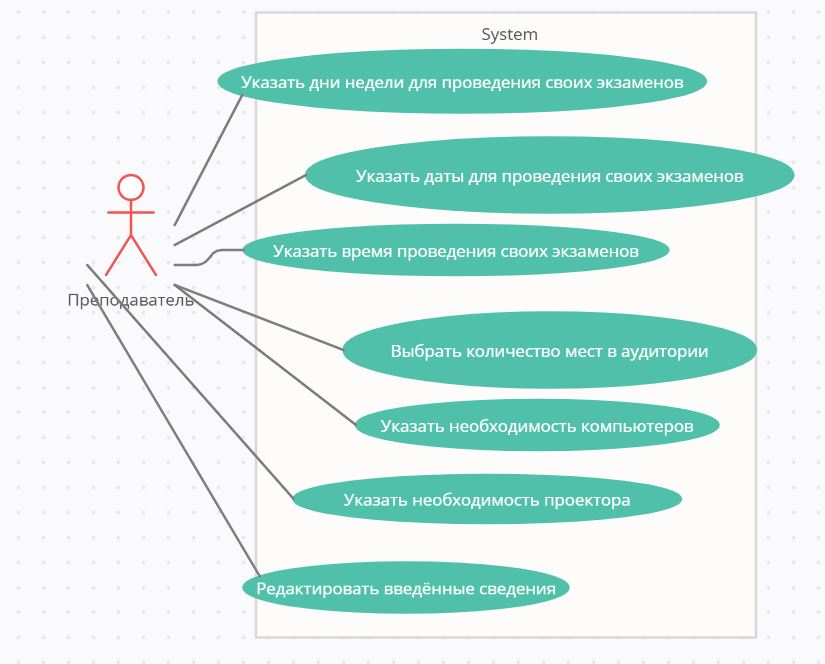
\includegraphics[scale=0.6, keepaspectratio=true] {my_folder/images/usecase1}
	\captionof{figure}{Use case диаграмма ППС}\label{fig:usecse1}  
	\vspace{\mfloatsep} % интервал  	
\end{minipage}

Возможности администратора показаны на диаграмме на рисунке \ref{fig:usecse2}.
Администратор заполняет общие сведения о сессии, такие как даты, время, доступные аудитории с указанием, сколько в них мест и есть ли там проектор и компьютеры и предстоящие экзамены по группам и преподавателям. Также, могут быть указаны аттестации, для которых уже определено время и место проведение. Это актуально, например, для событий, проводимых другими подразделениями университета. В возможности администратора помимо вышесказанного входит генерация формы сбора предпочтений преподавателей. 

\begin{minipage}{\textwidth}
	\centering
	\vspace{\mfloatsep} % интервал  	
	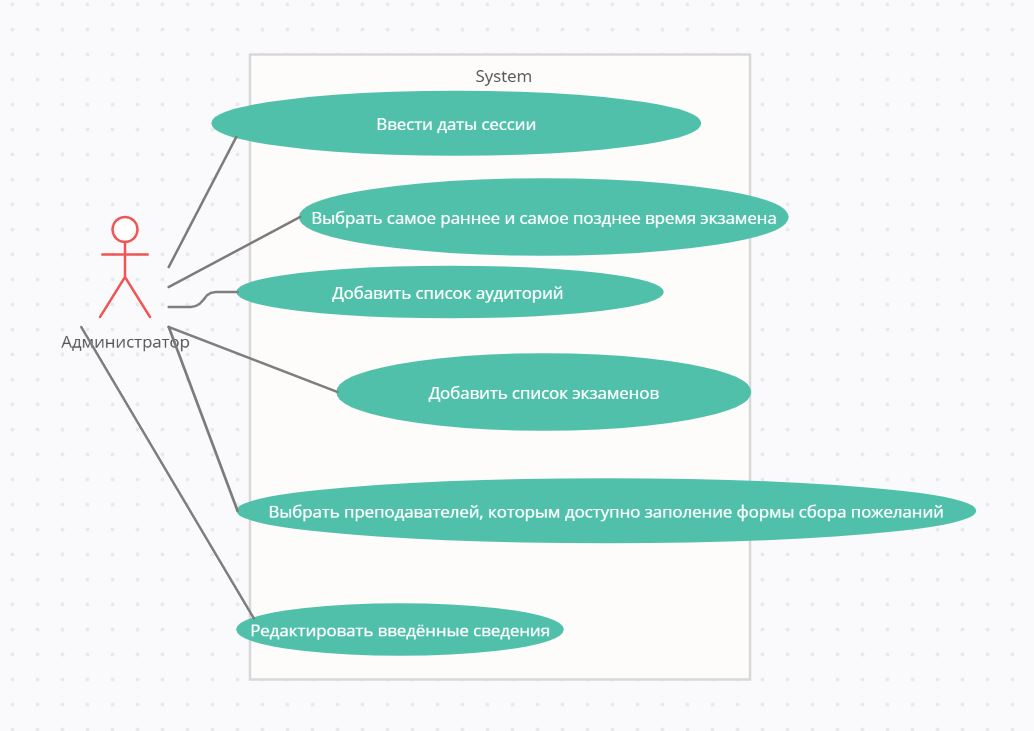
\includegraphics[keepaspectratio=true,scale=0.6] {my_folder/images//usecase2}
	\captionof{figure}{Use case диаграмма администратора}\label{fig:usecse2}  
	\vspace{\mfloatsep} % интервал  	
\end{minipage}

Таким образом, когда администратор заполнит все вышеперечисленные поля формы, в системе уже будет минимальный набор данных, необходимый для составления расписания. 
Далее, преподаватели могут заполнять свои формы с пожеланиями к своему расписанию. Незаполненная преподавателем форма не будет являться проблемой для системы. Пустая форма по умолчанию приравнивается к готовности преподавателя проводить экзамены и зачёты в любой день, в любое время. 

\subsection{Модель входных данных} \label{ch1:sec1:sub3}
\textbf{ПА: обычно раздел проектирования модели сущность-связь помещают в главы, связанные с разработкой. Рекомендую перенести.}

\textbf{ПА: не указаны типы отношений в модели. 1 к 1?}


Исходя из данных, которые необходимо учитывать при составлении расписания сессии, была спроектирована модель данных, соответствующая схеме базы данных для их хранения. Она представлена на схеме \ref{fig:bd}.

\begin{minipage}{\textwidth}
	\centering
	\vspace{\mfloatsep} % интервал  	
	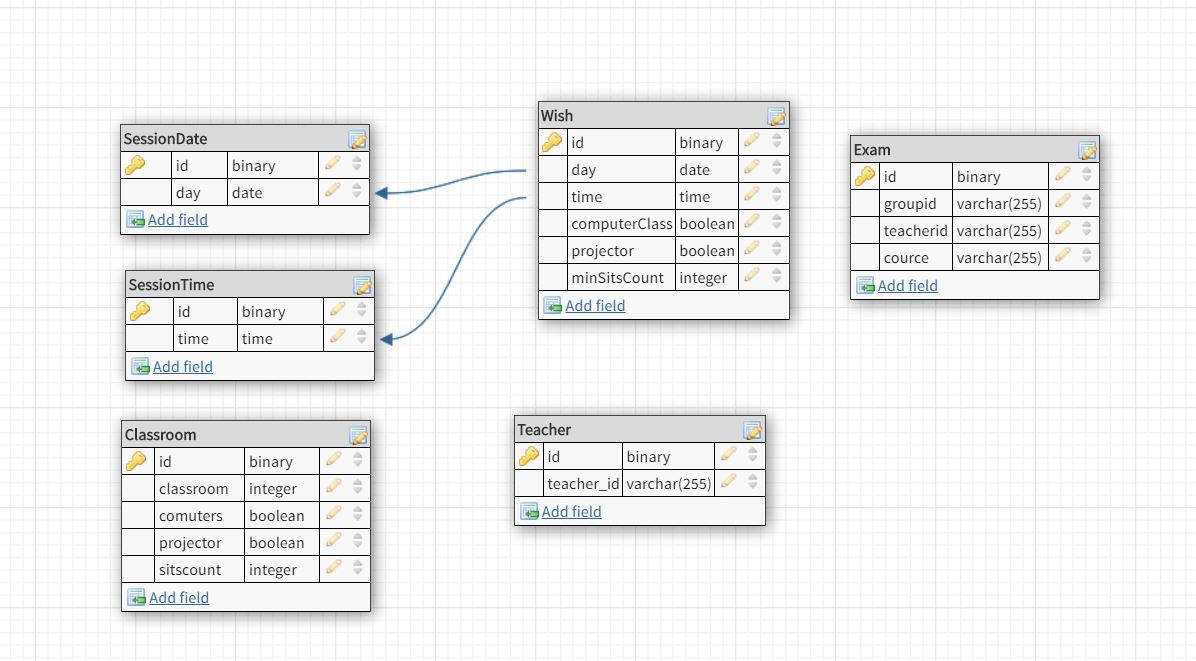
\includegraphics[ keepaspectratio=true, scale=0.4] {my_folder/images/bd}
	\captionof{figure}{Схема базы данных}\label{fig:bd}  
	\vspace{\mfloatsep} % интервал  	
\end{minipage}

Сущности схемы:

\begin{itemize}
	\item Teacher - таблица преподавателей.
	\begin{itemize}
		\item id - уникальный идентификатор
		\item name - имя
		\item prior - приоритет
	\end{itemize} 
	
	\item TeacherExamDate - таблица дат, которые преподаватель указывает, как доступные для проведения аттестаций. 
	\begin{itemize}
		\item id - уникальный идентификатор
		\item date - дата
		\item teacherId - id преподавателя
	\end{itemize} 
	
	\item TeacherExamTime - таблица времени, которое преподаватель указывает, как доступное для проведения аттестаций.
	\begin{itemize}
		\item id - уникальный идентификатор
		\item time - время
		\item teacherId - id преподавателя
	\end{itemize} 
		
	\item StudyGroup - таблица учебных групп.
	\begin{itemize}
		\item id - уникальный идентификатор
		\item level - курс
		\item name - номер
		\item size - кол-во студентов
	\end{itemize} 

	\item AttestationType - таблица типов аттестаций.
	\begin{itemize}
		\item id - уникальный идентификатор
		\item countPerDay - количество в день
		\item duration - длительность в часах
		\item pauseAfter -пауза в днях после аттестации
		\item pauseBefore - пауза в днях до аттестации
		\item type - название типа
	\end{itemize} 

	\item Classroom - таблица аудиторий с указанием есть ли там компьютеры или проектор и количеством мест.
	\begin{itemize}
		\item id - уникальный идентификатор
		\item classroom - номер кабинета
		\item computers - наличие компьютеров
		\item projector - наличие проектора
		\item sitscount - кол-во мест в аудитории
	\end{itemize} 

	\item SessionDate - таблица дат, в которые проводится сессия. Такой способ хранения данных о датах сессии был выбран вместо хранения даты начала и окончания, потому что зимняя сессия может состоять из нескольких интервалов, прерванных например новогодними праздниками.
	\begin{itemize}
		\item id - уникальный идентификатор
		\item date - дата
	\end{itemize} 

	\item SessionTime - таблица часов для проведения аттестаций.
	\begin{itemize}
		\item id - уникальный идентификатор
		\item time - время
	\end{itemize} 	

	\item ExternalExamLink - ссылки на google-таблицы, с аттестациями, для которых назначено время и место проведения. Они могут использоваться, например, для учёта аттестаций, которые назначаются другими подразделениями университета
\begin{itemize}
	\item id - уникальный идентификатор
	\item link - ссылка
\end{itemize} 

	\item Curriculum - таблица для хранения учебного плана.
\begin{itemize}
	\item id - уникальный идентификатор
	\item cource - название дисциплины
	\item semester - семестр, в который проводится аттестации
	\item specCode - специальность
	\item type - тип аттестации
\end{itemize} 

	\item Exam - таблица аттестаций, данные о которых вводятся вместе с данными о преподавателях. Используется при формировании расписании сессии заочников, когда по данным из расписания ruz, нельзя определить, кто должен проводить аттестации.
\begin{itemize}
	\item id - уникальный идентификатор
	\item cource - название дисциплины
	\item groupName - группа
	\item levels - семестр
	\item specName - специальность
	\item teacherName - преподаватель
	\item type - тип аттестации
\end{itemize} 
\end{itemize}

Описанные выше сущности соотносятся с данными, которые необходимо получать от пользователей. В процессе работы алгоритма составления расписания в персистентное хранилище записываются также следующие сущности: 
\begin{itemize}
	\item ResultLink - ссылки на google-таблицы, со сгенерированными ранее вариантами расписаний 
	\begin{itemize}
		\item id - уникальный идентификатор
		\item link - ссылка
	\end{itemize} 

	\item DateTimeClass - таблица доступных окон - дата+время+аудитория. В ней хранятся окна для проведения аттестаций, из которых исключены варианты, занятые другими занятиями.
	\begin{itemize}
		\item id - уникальный идентификатор
		\item date - дата
		\item time - время
		\item classroomId - id аудитории
	\end{itemize} 

	\item Event - таблица аттестаций, которые необходимо провести.
\begin{itemize}
	\item id - уникальный идентификатор
	\item cource - название дисциплины
	\item wishedClassroomType - необходимый тип аудитории
	\item teacherId - id преподавателя
	\item groupId - id учебной группы
\end{itemize} 
\end{itemize}


\section{Обзор российских систем составления расписания} \label{ch1:sec2}

\subsection{1С: ХроноГраф Расписание} 
Фирма «1С», занимающаяся разработкой ПО для бизнеса и образования, в качестве системы для автоматизации учебного планирования и составления расписания в разного рода организациях предлагает свою программу «1С: ХроноГраф Расписание» \cite{1с}.
«1С: ХроноГраф Расписание» позволяет:
\begin{itemize}
	\item cоставлять понедельное расписание организации или отдельных её подразделений;
	\item задавать периоды обучения с учётом нерабочих дней, каникул и разбиением на четные и нечётные недели;
	\item создавать черновое расписание, используя функцию «Предварительный расчёт».
\end{itemize}

Основной проблемой данной программы является несовместимость с другими платформами. «1С: ХроноГраф Расписание» - однопользовательская программа, и нельзя интегрировать её с web-приложением для возможности сбора данных напрямую от пользователей. Сложность составления расписания сессии в этой системе обуславливается также её ориентированностью на составление расписания по неделям без учёта специфики проведения аттестаций.

\subsection{Avtor}% сокращения не вводят в заголовках! 
Программа Avtor («АВТОРасписание»)  \cite{avtor} имеет несколько версий для различных учебных заведений: общеобразовательных школ, колледжей, техникумов, профессиональных училищ и ВУЗов. Это позволяет в подстроиться под специфику расписания конкретного типа образовательного учреждения, что является одним из её конкурентых преимуществ.

«АВТОРасписание» имеет достаточно широкий спектр применений. Этот программный продукт позволяет
\begin{itemize}
	\item cоставлять понедельное расписание для учебных групп с минимальным количеством окон;
	\item cоставлять расписание преподавателей с минимальным количеством окон;
	\item оптимально размещать занятия по аудиториям, учитывая их вместимость и оснащённость необходимым оборудованием;
	\item учитывать пожелания сотрудников к своему расписанию;
	\item разделять учебные группы на подгруппы;
	\item вносить ручные корректировки в расписание.
\end{itemize}

Преимуществом этой программы помимо прочего является возможность публиковать расписание обучающихся и преподавателей из самой системы «Автор» на сайте, внутреннем портале или на мультимедийных стендах образовательной организации. Но при этом импорт данных всё ещё производится вручную диспетчером, что не очень удобно для учебного заведения с большим штабом сотрудников, которые сами могли бы вносить свои пожелания в систему.

\subsection{Галактика Расписание учебных занятий}
%ПА: непонятно почему ``той же'' и почему это ``корпорация''?)
«Галактика Расписание учебных занятий» - часть системы управления ВУЗом организации Галактика  \cite{galaktica}. Этот программный продукт позволяет составлять расписание в ВУЗе, а также:

\begin{itemize}
	\item вычислять несколько десятков показателей эффективности расписаний;
	\item оптимально размещать занятия по аудиториям, учитывая их вместимость и оснащённость необходимым оборудованием;
	\item учитывать приоритет преподавателей, учебных групп и дисциплин;
	\item контролировать пересечение расписаний для преподавателей, учебных групп и подгрупп во избежание «накладок»;
	\item контролировать длительность занятий;
	\item вручную бронировать аудиторный фонд;
	\item учитывать план изучения дисциплин для выстраивания их в правильном порядке.
\end{itemize}

«Галактика Расписание учебных занятий» - серьёзный инструмент для формирования расписания в высших учебных заведениях, учитывающий множество факторов при его составлении и имеющий удобную систему отчётности. На данный момент эта программа наиболее полно решает проблему автоматической генерации расписания российских ВУЗов, но и она не имеет интерфейса для прямого импорта пожеланий преподавателей прямо в систему. Компания «Галактика» помимо прочего предлагает техническое сопровождение своего ПО, но это учитывается при расчёте стоимости лицензии на использование программы.

Составление расписания в СПбПУ производится при активном использовании данной программы.
	
\section{Обзор зарубежных систем составления расписания} \label{ch1:sec3}	

\subsection {Apereo UniTime}
UniTime от компании Apereo \cite{unitime} - система автоматического создания расписания западных высших учебных заведений. Она учитывает, что студенты могут выбирать себе индивидуальный набор курсов. %, чего не происходит в российских ВУЗах, где обучение происходит по плану образовательных программ направлений.
%ПА: это не так, у нас есть модули мобильности и даже дисциплины по выбору (последние как правило только на бумаге по выбору), но лучше не офишировать.

UniTime даёт возможность:
\begin{itemize}
	\item автоматически генерировать расписание курсов и экзаменов;
	\item минимизировать конфликты студенческих курсов;
	\item вносить ручные корректировки в расписание.
\end{itemize}

Эта программа имеет понятный web-интерфейс и может быть интегрирована в другую систему, но она не позволяет преподавателям вносить данные о своей занятости, чтобы учесть их при составлении расписания. Неприспособленность программы под составление расписания для групп, а не для конкретных студентов делает её менее удобной, чем российские аналоги.

\subsection {Lantiv Scheduling Studio} 
Программа «Scheduling Studio» \cite{lantiv} от компании Lantiv представляет собой систему совместной работы над расписанием и реализует следующие задачи:

\begin{itemize}
	\item совместный доступ к редактированию расписания ВУЗа;
	\item оффлайн редактирование с возможностью синхронизации после появления в сети;
	\item цветовое выделение накладок расписания;
	\item cоставление расписания на различные временные периоды: неделя, семестр, четверть, год;
	\item копирование составленных элементов расписания на другие периоды.
\end{itemize}

Данный программный продукт имеет приятный и понятный интерфейс, но не имеет модуля автоматической генерации расписания, из-за чего основная часть работы всё ещё ложится на плечи диспетчеров. «Scheduling Studio» удобно использовать для составления нетривиального расписания, которое меняется от недели к неделе и плохо вписывается в шаблон школьного расписания или расписания учебных занятий ВУЗа, например. Но для составления расписания сессии требуется большая степень автоматизации, чем предлагается этим ПО.

\section{Выводы} \label{ch1:conclusion}
Сведения о возможностях каждого из описанного в параграфах	\ref{ch1:sec2} и \ref{ch1:sec3} сведём в таблицу \ref{tab:1.4.1}.
\begin{table} [htbp]
	\centering\small
	\caption{Сравнение систем составления расписания}%
	\label{tab:1.4.1}	
	\begin{tabular}{|p{0.18\linewidth}|p{0.1\linewidth}|p{0.15\linewidth}|p{0.1\linewidth}|p{0.08\linewidth}|p{0.1\linewidth}|p{0.1\linewidth}|}
		\hline
		&Учитывает пожелания ППС&Интегрируется с сайтами ВУЗов&Имеет возможность задавать нетривиальное расписание&Плата за использование&Генерация предварительного расписания&Открытый исходный код\\
		\hline
		1С: ХроноГраф Расписание&+&-&-&+&+&-\\ \hline
		Avtor&+&-&+&+&+&-\\ \hline
		Галактика Расписание учебных занятий&+&+&+&+&+&-\\ \hline
		Apereo UniTime&-&+&+&-&+&+\\ \hline
		Lantiv Scheduling Studio&-&-&+&+&-&-\\ \hline	
	\end{tabular}
\end{table}

Видно, что среди систем составления расписания для составления предварительного расписания сессии лучше всего могла бы подойти программа «Галактика Расписание учебных занятий», так как она удовлетворяет большинству требований, но при этом она, как и почти всё представленное в таблице ПО, требует оплату за использование. Также среди представленных программных продуктов все, кроме одного, не предоставляют открытый доступ к исходному коду. 
В рамках данной работы необходимо было разработать программу, удовлетворяющую всем перечисленным в таблице критериям.

\textbf{ПА: надо мотивировать более точно, почему не подошел вариант с доработкой Apero. Может быть там предусмотрен режим составления ТОЛЬКО индивидуального расписания? или не развит какой-то функционал?}	         	 % Глава 1
\ContinueChapterBegin % размещать главы <<подряд>> 
\chapter{Алгоритмы составления расписания сессии} \label{ch2}
	
% не рекомендуется использовать отдельную section <<введение>> после лета 2020 года
%\section{Введение} \label{ch2:intro}

Глава посвещена обзору алгоритмов, которые можно применять для составления расписания сессии, а также для оптимизации этого процесса. 

В параграфе \ref{ch2:sec1} приведена постановка задачи составления расписания сессии, далее в параграфе \ref{ch2:sec2} рассморены два возможных режима составления расписания, а в параграфах \ref{ch2:sec3} и \ref{ch2:sec4} - алгоритмы, используемые для решения данной задачи. 

\section{Постановка задачи составления расписания сессии} \label{ch2:sec1} 

Для составления расписания учебной сессии в университете необходимо каждой запланированной аттестации подобрать день, время и аудиторию проведения. 
Известны доступные аудитории и множество аттестаций, которые необходимо провести в рамках сессии. Для каждой аудитории известно время ее доступности. Для каждого типа аттестации определена длительность, максимальное количество в день и количество дней отдыха до и после её проведения. Нужно составить расписание сессии так, чтобы общая эффективность расписания была наибольшей. Далее введём метематические обозначения для названных выше параметров, формализуем ограничения и определим, какое расписание будет являться оптимальным.

\subsection{Обозначения} 

Составим расписание сесии для g учебных групп, каждая из которых характеризуется номером и количеством учащихся в ней студентов. 

Множество номеров учебных групп: 
\begin{align}
	& Gr\ =  \{ gr_1,...,gr_g \} 
\end{align}

Количество студентов в соответсвующей учебной группе: 
\begin{align}
	& S\ =  \{ s_1,...,s_g \} 
\end{align}

В данной задаче необходимо учитывать пожелания преподавателей, поэтому каждый преподаватель помимо ФИО должен характеризоваться множеством удобных для него дней и часов проведения аттестаций. Также преподавателям необходимо прописывать приоритет, чтобы в случаях, когда нельзя удовлетворить пожеланиям всех преподавателей, в первую очередь будут учитываться пожеланиям именно преподавателей с большим приоритетом.

Множество, состоящее из p имён преподавателей ВУЗа:
\begin{align}
	& T\ =  \{t_1,...,t_p \} 
\end{align}

Приоритеты соответсвующих преподавателей:
\begin{align}
	& Pr\ =  \{pr_1,..,pr_p \} 
\end{align}

Множество из q дней, которые преподаватель t выбрал возможными для проведения им аттестаций:
\begin{align}
& Td_t\ =  \{td_{t1},...,td_{tq} \} 
\end{align}

Множество из c часов, которые преподаватель t выбрал возможными для проведения им аттестаций:
\begin{align}
& Tt_t\ =  \{tt_{t1},...,tt_{tc} \} 
\end{align}

Важно также учитывать правила проведения сессий, ограничивающие количество аттестаций в день и определяющие, сколько дней отдыха нужно оставить группе до и после аттестации.

Определим множество из y типов аттестаций (экзамен, зачёт и т.п.):
\begin{align}
	& A\ =  \{a_1,...,a_y\} 
\end{align}

Количество дней отдыха перед (Pb)  и после (Pa) проведением аттестации каждого типа:
\begin{align}
	& Pb =  \{pb_1,...,pb_y\}\\ 
	& Pa =  \{pa_1,...,pa_y\} 
\end{align}

Длительность каждого типа аттестации в часах:
\begin{align}
	& Ad =  \{ad_1,...,ad_y\}
\end{align}

Максимальное количество аттестаций каждого типа в день:
\begin{align}
	& Ac =  \{ac_1,...,ac_y\} 
\end{align}

При выборе аудиторий для проведения аттестаций необходимо полагаться на их размер и техническую оснащённость. Опрелелим множество из u номеров аудиторий:
\begin{align}
	& R =  \{r_1,...,r_u\} 
\end{align}

Типы соответсвующих аудиторий (компьютерный класс, имеет проектор и т.п.):
\begin{align}
	& Rt =  \{rt_1,...,rt_y\} 
\end{align}

Количество мест в соответсвующих аудиториях:
\begin{align}
	& Rs =  \{rs_1,..,rs_y\} 
\end{align}

Аттестации, которые необходимо провести в течение сессии описываются учбной группой, дисциплиной и преподавателями, которые должны провести данную аттестацию. Так же для каждой аттестации необходимо указать её тип и тип аудитории, в которой она должна проводиться.

Множество аттестаций:
\begin{align}
	& {E} =  \{ e_1,...,e_k\}
\end{align}

Множества групп (Еg) и дисциплин (Ec) для каждой из k аттестаций:
\begin{align}
	& Eg =  \{ eg_i\in{}Gr , \forall  i \in{} \{1,..,k\} \} \\ 
	& {Ec} =  \{ ec_1,...,ec_k\}
\end{align}

Множества типов аттестаций и типов аудиторий для каждой из k аттестаций:
\begin{align}
	& Ea =  \{ ea_i\in{}A , \forall  i \in{} \{1,..,k\} \} \\ 
	& Er =  \{ er_1,...,er_k\}
\end{align}

Множество, состоящее из преподавателей, проводящих аттестацию e:
\begin{align}
	& Et_e =  \{ et_{ei}\in{}T , \forall  i \}
\end{align}

Каждой аттестации необходимо сопоставить дату, часы и аудиторию для проведения. Декартово произведение всех возможных дат, часов и свободных кабинетов представляет собой множество потенциальных окон для проведения аттестаций.

Множество окон:
\begin{align}
	& W =  \{w_1,..,w_n\} 
\end{align}

${wd_i \in D}$ - календарный день, соответствующий окну i;

${wh_i \in H}$ - время, соответствующее окну i;

${wc_i\in{}R , \forall  i \in{} \{1,...,n\}}$ - аудитория, соответствующая окну i.


Введём множество Solutions, состоящее из функций булевых переменных, которые принимают значение 1, если за i-ей аттестацией бронируется j-е окно:
\begin{equation}
	S(i,j) = 
	\begin{cases}
		1 &\text{ the attestation $e_i$ is held in window $w_j$} \\
		0 &\text{ the attestation $e_i$ is not held in window $w_j$}
	\end{cases}
\end{equation}

Таким образом, необходимо найти значения функции ${S \in Solutions}$ для ${ \forall  i  \in \{1,..,k\}}$  и  ${ \forall j \in \{1,..,n\}}$. Множество пар <i,j>, для которых S(i,j) = 1, представляют собой расписание сессии - соотвествие аттестации дню, врмени и аудитории.

Программно описанные в этом параграфе множестве реализованы в качестве классов, представленных] в приложении \ref{appendix-classes}.

\subsection{Ограничения}
Задача составления расписания сессии имеет ряд физических ограничений, а также ограничений, обусловленных правилами проведения сессии. Соблюдение этих ограничений позволит составить корректное расписание сессии:

Во-первых, в одной аудитории в одно время может проводиться только одна аттестация:
\begin{align}
	& \forall  j \in \{1,..,n\} \sum_{i=1}^kS(i,j) = 1
\end{align}

Каждая аттестация в период сессии должна проводиться единожды, так как в данном случае не рассматривается расписание дополнительной сессии:
\begin{align}
	& \forall  i \in \{1,..,k\} \sum_{j=1}^nS(i,j) = Ad_ea_i
\end{align}

Преподаватель не должен отрабатывать в определённый день больше некоторого количества часов x:
\begin{align}
	& \forall b \in \{1,..,p\} : \sum_{\forall i \in \{1,..,k\}, et_{ia}=t_b}\sum_{\forall j \in \{1,..,n\}}\sum_{ \forall u \in d_u \in D, wd_j = d_u }S(i,j) <= x
\end{align}

Любая группа не может сдавать аттестации любого типа в день больше, чем макисмальное число, обусловленное типом аттестации:
\begin{align}
\begin{multlined}
	 \forall b \in \{1,..,g\}, \forall j \in \{1,..,n\}, \forall m \in \{1,..,y\} :\\ \sum_{\forall i \in \{1,..,k\}, et_i = a_m,  eg_i=gr_b}\sum_{ \forall d \in D, wd_j = d }S(i,j) <= ac_m * ad_m
\end{multlined}
\end{align}

Любая группа перед любой своей аттестацией не должна иметь аттестаций в окно отдыха перед аттестацией этого типа:
\begin{align}
	\begin{multlined}
		\forall b \in \{1,..,g\}, \forall i \in \{1,..,k\} eg_i=gr_b:\\
		 \max_{\forall j \in \{1,..,n\}, ed_j < ed_i}(ed_j) <ed_i-pb_{et_i}
	\end{multlined}
\end{align}

Любая группа после любой своей аттестацией не должна иметь аттестаций в окно отдыха после аттестацией этого типа:
\begin{align}
	\begin{multlined}
		\forall b \in \{1,..,g\}, \forall i \in \{1,..,k\} eg_i=gr_b:\\
		\min{\forall j \in \{1,..,n\}, ed_j > ed_i}(ed_j) >ed_i-pa_{et_i}
	\end{multlined}
\end{align}

Каждая аттестация должна проводиться в аудитории равной и или превосходящей по вместимости размеру группы:
\begin{align}
	& \forall i \in \{1,...,k\}, \forall j \in \{1,..,n\} : s_{eg_i} > rs_{wc_j} \rightarrow S(i,j) = 0
\end{align}

Каждая аттестация не может проводиться в аудитории с оснащённостью меньшей ожидаемой:
\begin{align}
	& \forall i \in \{1,...,k\}, \forall j \in \{1,..,n\} : er_i < rt_{wc_j} \rightarrow S(i,j) = 0
\end{align}

Чтобы составить расписание, комфортное для преподавательского состава, учтём некоторые ограничения связанные с предпочтениями преподавателей. Эти огнаричения уже не столь критичны, как перечисленные выше, так как их нарушение не влечёт за собой нарушение правил или законов физики, но их наличие делает расписание более удобным для сотрудников.

Каждый преподаватель волен указать список календарных дней, в которые он готов принимать аттестации. Идеальное расписание предполагает, что любой преподаватель проводит все свои аттестации только в дни из этого списка:
\begin{align}
	\label{eq:T1}
	& \forall t \in T, \forall d \in D : d \notin Td_t \rightarrow S(i,j) = 0
\end{align}

Также, преподаватель может указать удобные для него часы провеления аттестаций. Идеальное расписнаие учитывает это и располагает аттестации так, чтобы они затрагивали только выбранные часы каждого преподавателя:
\begin{align}
	\label{eq:T2}
	& \forall t \in T, \forall h \in H : h \notin Tt_h \rightarrow S(i,j) = 0
\end{align}

Данная задача относится к классу NP-полных задач, а значит в худшем исходе придётся перебрать все возможные k аттестаций и n окон в качестве аргументов функции S(i,j), где выполняются все описанные выше ограничения. Обобщим их для функции S:

\begin{equation}
	\label{eq:S}
	S(i,j) = 
	\begin{cases}
		\forall  j \in \{1,..,n\} \sum_{i=1}^kS(i,j) = 1;\\
		\forall  i \in \{1,..,k\} \sum_{j=1}^nS(i,j) = Ad_ea_i;\\
		\forall b \in \{1,..,p\} : \\ \sum_{\forall i \in \{1,..,k\}, et_{ia}=t_b}\sum_{\forall j \in \{1,..,n\}}\sum_{ \forall u \in d_u \in D, wd_j = d_u }S(i,j) <= x;\\
		\forall b \in \{1,..,g\}, \forall j \in \{1,..,n\}, \forall m \in \{1,..,y\} :
		\\ \sum_{\forall i \in \{1,..,k\}, et_i = a_m,  eg_i=gr_b}\sum_{ \forall d \in D, wd_j = d }S(i,j) <= ac_m * ad_m;\\
		\forall b \in \{1,..,g\}, \forall i \in \{1,..,k\} eg_i=gr_b: \\ \max\limits_{\forall j \in \{1,..,n\}, ed_j < ed_i}(ed_j) <ed_i-pb_{et_i};\\
	\forall b \in \{1,..,g\}, \forall i \in \{1,..,k\} eg_i=gr_b:\\ \min\limits_{\forall j \in \{1,..,n\}, ed_j > ed_i}(ed_j) >ed_i-pa_{et_i};\\
	\forall i \in \{1,...,k\}, \forall j \in \{1,..,n\} : s_{eg_i} > rs_{wc_j} \rightarrow S(i,j) = 0;\\
	\forall i \in \{1,...,k\}, \forall j \in \{1,..,n\} : er_i < rt_{wc_j} \rightarrow S(i,j) = 0\\
	\end{cases}
\end{equation}

Оптимальным расписанием будет такое, где минимальное количество пожеланий преподавателей игнорируется. Таким образом, сведём задачу к поиску такого расписания S, на котором выполняется слудеющий минимум:

\begin{align}
	\label{eq:T}
	& \min_{\forall S \in Solutions}(\sum_{\forall i \in \{1,...,k\}, \forall j \in \{1,..,n\}, wd_j \notin Td_{et_i}, wh_j \notin Th_{et_i}}(S(i,j)*pr_{et_i}))
\end{align}

Видно, что идеальными расписаниями будут те, где учитываются пожелания всех преподавателей, так как в этом случае точно достигается наименьшее значение минимума формулы \eqref{eq:T} = 0. 

 Для решения данной задачи рассмотрим алгоритмы динамического и линейного программирования, алгоритм на графах, эволюционный алгоритм и метод численной оптимизации.

\section{Режимы алгоритмов составления расписния} \label{ch2:sec2} 

Алгоритмы составления расписания можно использовать в двух режимах: инкрементальном и пакетном (batch-режим). В данном разделе рассмотрим, что из себя представляет каждый из этих режимов и почему пакетный режим больше подходит для решения задачи составления расписания сессии.

\subsection{Инкрементальный режим}

Инкрементальным режимом назовём выполнение алгоритма многократно при появлении новых данных. В контексте данной задачи это означает, что каждый раз, когда новый преподаватель будет добавлять информацию о своих предпочтениях, алгоритм будет просчитывать возможные варианты расписания с учётом:
\begin{itemize}
	\item уже имеющихся данных, которые имеют приоритет, перед новыми;
	\item внесённых преподавателем изменений.
\end{itemize}

Так, при каждом новом пересчёте уже составленные расписания преподавателей считаются утверждёнными, что даёт возможность не считать их заново, тем самым ускорив работу алгоритма.

Из преимуществ данного подхода можно выделить возможность преподавателя, не дожидаясь других, увидеть своё расписание. Также, с точки зрения организации, плюсом можно считать стимул преподавателей как можно раньше заполнить форму сбора информации, чтобы иметь приоритет перед другими. Таким образом появляется возможность раньше закончить процесс составление расписания. 

Недостатки данного режима более существенны на практике, чем его преимущества, так как основным недостатком является закрепление наиболее удобного расписания за теми, кто заполнил форму сбора раньше остальных, что может повлечь коллизии. Можно рассмотреть случай, когда первый преподаватель, заполнивший форму сбора, выбирает большое окно для проведения экзаменов и алгоритм бронирует за ним несколько определённых случайных дат, а остальные оставляет свободными. Тогда второй преподаватель, уезжающий на конференцию в свободные даты и готовый провести экзамены в даты, занятые первым, уже не сможет это сделать, потому что у первого преподавателя приоритет, и его уже нельзя подвинуть на сводные даты.

\subsection{Пакетный режим}

Пакетным режимом в данном случае будет единоразовая обработка всех полученных сведений. Для этого необходимо определить дедлайн для сбора пожеланий преподаватель, при наступлении которого составить предварительное расписание для всех за один вызов алгоритма. 

Преимуществом такого подхода является возможность установить приоритеты преподавателей и групп, на основе которых можно решать коллизии в случае невозможности нахождения идеального решения, учитывающего пожелания каждого. 

Недостатком такого подхода можно назвать невозможность до дедлайна получить расписание, но в реальности это не будет глобальным минусом, потому что составленное таким образом предварительное расписание, всё равно, в последствии может быть скорректировано вручную. 

Таким образом, из двух рассмотренных режимов для решения задачи составления расписания больше подходит именно пакетный, потому что его преимущества более значимы, а единственный недостаток не играет роли на практике, в отличие от описанных недостатков инкремениального режима.

\section{Обзор алгоритмов составления расписания сессии} \label{ch2:sec3} 
\subsection{Обход графа в глубину для поиска идеальных решений}

Задача составления расписания сессии является NP-полной, как, например, задача обхода графа, для которой существует множество классических алгоритмов, решающих её. Алгоритм обхода графа в глубину \cite{dfs} является одним из них. Но чтобы применить этот алгоритм для составления расписания, необходимо свести эту задачу к задаче построения графа, у которого в качестве вершин выступают элементы расписания - аттестации и временные окна для их проведния. Наличие ребра обуславливается выполнением двух следующих условий:
\begin{itemize}
	\item ребро из вершины с аттестацией i из отсортрованного списка аттестаций E, может быть соединено только с аттестацией i+1 из E;
	\item ребро из вершины <i,j> с аттестацией i и окном j в вершину <i+1, q> может существовать, если выполняются условия формул \eqref{eq:S}, \eqref{eq:T1} и \eqref{eq:T2} для S(i+1, q) при n=i+1.
\end{itemize}

 Тогда решением будет являться связный граф состоящий из k вершин - пар аттестаций и временных окон, отведённых для этих аттестаций.

Основная идея обхода в глубину – когда возможные пути по ребрам, выходящим из вершин, разветвляются, нужно сначала полностью исследовать одну ветку и только потом переходить к другим веткам. Сложность классического обхода в глубину с матричным заданием графа равна ${O(m^2)}$, где {$m=n*k$} - количество вершин. Но так как известно, что доступность рёбер для каждой из вершин с аттестацией i огрничена n вершинами с аттестацией i+1, сложность снизится до ${O(n^2 * k)}$. Но так как для проверки остальных условий необходимо проверять i предыдущих вершин графа, сложность останется ${O(n^2 * k*\log(k))}$.

 В процессе решения занчениями функции S(i,j) будет заполняться булева матрица. Важно помнить, что значение 1 в ячейке может быть проставлено, только при соблюдении ограничений системы \eqref{eq:S} , и стоит заметить, что выполнение ограничения, что в одной аудитории в одно время может проводиться только одна аттестация, влечёт за собой наличие в одном столбце матрицы не более одного значения 1, из-за чего матрицу можно заменить на целочисленный массив, где индексы соответствуют индексу возможного окна, а значения - индексу события, которое будет там проведено.

Будем считать, что идеальное решение найдено, если в каждой строке матрицы есть значение 1 или каждое число от 0 до k встречается в массиве решения, что означает, что каждую аттестацию можно сопоставить какому-то окну ${w_j}$ c учётом перечисленных выше ограничений. Такое решение добавляется в список всех идеальных решений. Даллее представлен псевдокод процедуры FindSolutions \ref{alg:algoFindSol}. , которая реализует алгоритм обхода графа в глубину. Заметим, что в списке доступных окон W все элементы отсортированы по дням, кабинетам и часам, чтобы легко можно было оценивать занятость одного кабинета несколько часов подряд.

	\begin{algorithm} 
	\SetKwFunction{algoFindSol}{} 
	\SetKwProg{myalg}{Algorithm }{ FindSolutions}{}
	\nonl\myalg{\algoFindSol}{
		\KwInput{$\cont[E], \cont[W], k = |\cont[E]|, n = |\cont[W]| $} 
		\KwOutput{$\cont[Solutions]$} 
		{$Solutions \leftarrow \{\}, $}
		{$S \leftarrow [], $}
			{$i \leftarrow 0$}\\
		\While{$i < k$}{
			{$time = NextTime(i)$} \\
			\For{$\forall u \in {0,...,k }$}{
				\If{$ S[u] = i $ } {
					{$S[u] \leftarrow -1$} \\
				}	
			}
			{$nextTime = FindNextStartTime(i,time)$}\\
			\If{$nextTime = -1$ }{
				\If{$i = 0$ }{
					\Return {$ Solutions$}
				} \Else {
					{$i \leftarrow i-1$}\\
				}
			} \Else {
		   		{$duration = ed_i $}\\
		   		\For{$\forall b \in \{nextTime,...,nextTime + duration\} $} {
		   			{$S[b] \leftarrow i$}\\
		   		}
				{$i \leftarrow i+1$}\\
			}
			\If{$i = k$ }{
					{$Solutions \leftarrow Solutions \bigcup S$}\\
					{$i \leftarrow i-1$}\\
			} 
		}
	\Return {$ Solutions$}\\
	}
	\caption{Псевдокод алгоритма \texttt{DFS} для составления расписания}\label{alg:algoFindSol}
\end{algorithm} 

В процедуре FindNextStartTime \ref{alg:algoFindNextPr} проводится проверка условий из формулы \eqref{eq:S}, чтобы подобрать следующее подходящее ребро, исходящее из указанной вершины. В случае, если для вершины не существует исходящего ребра, которое удовлетворяет всем условиям, данная процедура вернёт значение -1, в противном случае вернёт следующее ребро. В данной функции также происходит проверка условий из формул \eqref{eq:T1} и \eqref{eq:T2}, чтобы обеспечить поиск идеального решения, удовлетворяющего пожланиям всех преподавателей. 

\begin{algorithm} 
\SetKwFunction{algoFindNext}{} 
	\SetKwProg{myalg}{Function}{ FindNextStartTime}{}
	\nonl\myalg{\algoFindNext}{
		\KwInput{$event, time, \cont[E], \cont[W], \cont[S], k = |\cont[E]|, n = |\cont[W]| $} 
		\KwOutput{$t$} 
		\If{$ time < 0$ } {
			\Return -1 \\
		}	
		\For{$i \in \{time,...,k\} $}{
			{$w \leftarrow W[i]$}\\
			\If {$S[i] = -1 
				\land rt_{w} = er_{event}  
				\land i + ad_{event} < n 
				\land s_{eg_{event}} <= er_{w}
				\land er_{w} = er_{W[i+ad_{event}]}
				\land ed_{w} = ed_{W[i+ad_{event}]}
				\land wd \in Td_{event}
				\land wt \in Tt_{event}
				\land wt+ed_{w} \in Tt_{event}$}
			{
				{$teacherTime \leftarrow 0, countPerDay \leftarrow 0, 	j \leftarrow 0 $} \\
		\While{$i < k$}{
			\If {$S[j] = -1 $}{
				{$j \leftarrow j+1$}\\
				{$continue$}\\
			}
			\If {$w = S[j] 	\land wt \in et_{solution[j]}$}{
				{$break$}\\
			}
			\If {$et_{S[j]} = et_{event}$}{
			{$teacherTime=teacherTime+1$}\\
			\If {$teacherTime > maxTimePerDay - ed_{event}$}{
				{$break$}\\
			}
		}
		\If {$eg_{S[j]} = eg_{event}$}{
			\If {$(ea_{S[j]=ea_{event}}) \land (wd = ed_{S[j]})$}{
				{$ countPerDay \leftarrow countPerDay+1 $} \\
				\If {$(ac_{et_{event}} < countPerDay) \lor (wt-pb_{ea_{event}}<=wd_{S[j]}\land wt+pa_{ea_{event}}>=wd_{S[j]})$}{
						{$break$}\\
					}
		}
			{$k \leftarrow k+1$}
		}	
	}
	\If{$j = n$}{
		 \Return {$i$} \\
	}
			}
		}
	\Return -1
	}
\caption{Проверка условий формул \eqref{eq:S}, \eqref{eq:T1} и \eqref{eq:T2}}\label{alg:algoFindNext}
\end{algorithm} 
\FloatBarrier
\subsection{Алгоритм обхода графа в глубину с учётом приоритетов преподавателей}

На практике возникают ситуации, когда недостаток аудиторий и накладки в личных расписаниях преподавателей не позволяют найти такое расписание, которое удовлетворит всем пожеланиям. По этой причине приходится учитывать приоритеты ограничений и минимизировать потери по формуле \eqref{eq:T}. 

Существует ряд ограничений, поступиться с которыми нельзя. В их число входят правила проведения аттестаций и физические условия, связанные с проведением экзаменов в аудиториях, опписанные в формуле \eqref{eq:S}. Но есть и менее жёсткие факторы - это пожелания преподавателей к датам и времени экзаменов. 

Каждый преподаватель указывает дни и время, когда ему было бы удобно присутствовать на аттестации. В некоторых случаях удобство эквивалентно тому, что в остальные дни преподаватель в принципе не может принимать экзамены. Приоритет таких ограничений должен быть выше, чем у случаев, когда преподавателю просто комфортнее было бы присутствовать на экзаменах в определённые дни.

Для этого было введено множество приоритетов Pr, где больший приоритет соответствует большему влиянию учёта пожеланий преподавателя на потери функции \eqref{eq:T}. Система приоритетов в случае появления коллизий при составлении расписания позволит в первую очередь пытаться нарушить только пожелания с наименьшим приоритетом и только, если это необходимо, с более высокими.

Модернизируем алгоритм поиска «идеального» решения:

Для этого нужно хранить массив ignoreWishes, в котором будут фиксироваться те аттестации, для которых приходится искать решения без учёта предпочтений преподавателей.

Также, в алгоритме \ref{alg:algoFindSolPr} на строке \ref{step:sortE} необходимо отсортировать массив аттестаций по приоритетам преподавателей, чтобы искать решения без учёта высокоприоритетных преподавателей лишь в последнюю очередь. 

Метод поиска решений FindSolutions \ref{alg:algoFindSolPr} теперь содержит условный оператор, который в случае определения того, что идеального решения найти не удаётся, переходит в режим игнорирования пожеланий преподавателя для конкретного события. Для этого в массиве ignoreWishes выставляется true по индексу, соотвествующему этому событию.

\begin{algorithm} 
	\SetKwFunction{algoFindSolPr}{} 
	\SetKwProg{myalg}{Algorithm }{ FindSolutions}{}
	\nonl\myalg{\algoFindSolPr}{
		\KwInput{$\cont[P], \cont[E], \cont[W], k = |\cont[E]|, n = |\cont[W]| $} 
		\KwOutput{$\cont[S]$} 
		{$ignoreWishes \leftarrow [], $}
		{$S \leftarrow [], $}
		{$i \leftarrow 0$}\\
		{$Sort(E)$\label{step:sortE}} \\
		\While{$i < k$}{
			{$time = NextTime(i)$} \\
			\For{$\forall u \in {0,...,k }$}{
				\If{$ S[u] = i $ } {
					{$S[u] \leftarrow -1$} \\
				}	
			}
			{$nextTime = FindNextStartTime(i,time)$}\\
			\If {$ ignoreWishes[i] = False \land nextTime = -1$ }{
				{$ignoreWishes[i] = True$} \\
				{$nextTime = FindNextStartTime(i,0)$}\\
			}
			\If{$nextTime = -1$ }{
				\If{$i = 0$ }{
					\Return {$null$}
				} \Else {
				{$ignoreWishes[i] = False$}\\
					{$i \leftarrow i-1$}\\
				}
			} \Else {
				{$duration = ed_i $}\\
				\For{$\forall b \in \{nextTime,...,nextTime + duration\} $} {
					{$S[b] \leftarrow i$}\\
				}
				{$i \leftarrow i+1$}\\
			}
		}
		\Return {$ S$}\\
	}
	\caption{Псевдокод алгоритма \texttt{DFS} для составления расписания c учётм приоритетов преподавателей}\label{alg:algoFindSolPr}
\end{algorithm} 

Метод поиска следующего подходящего времени и аудитории теперь может работать в двух режимах. В режими игнорирования рассматриваются только те окна, которые хотя бы в какой-то мере не удовлетворяют пожеланиям преподавателя. Для этого в алгоритме \ref{alg:algoFindNextPr} в строке \ref{step:ignor} используется логический оператор XOR между результатом проверки соблюдения пожеланий преподавателя и значением в массиве игнорирования.

\begin{algorithm} 
	\SetKwFunction{algoFindNextPr}{} 
	\SetKwProg{myalg}{Function}{ FindNextStartTime}{}
	\nonl\myalg{\algoFindNextPr}{
		\KwInput{$event, time, \cont[E], \cont[W], \cont[S], k = |\cont[E]|, n = |\cont[W]|, ignoreWishes $} 
		\KwOutput{$t$} 
		\If{$ time < 0$ } {
			\Return -1 \\
		}	
		\For{$i \in \{time,...,k\} $}{
			{$w \leftarrow W[i]$}\\
			{$teacherWish \leftarrow (wd \in Td_{event}
				\land wt \in Tt_{event}
				\land wt+ed_{w} \in Tt_{event}) \nsim ignoreWishes[i]$ \label{step:ignor}}\\
			\If {$S[i] = -1 
				\land rt_{w} = er_{event}  
				\land i + ad_{event} < n 
				\land s_{eg_{event}} <= er_{w}
				\land er_{w} = er_{W[i+ad_{event}]}
				\land ed_{w} = ed_{W[i+ad_{event}]}
				\land teacherWish$}
			{
			...\\
				}
				\If{$j = n$}{
					\Return {$i$} \\
				}
			}
		\Return -1
	}
	\caption{Проверка условий формулы \eqref{eq:S} с учётом режима игнорирования}\label{alg:algoFindNextPr}
\end{algorithm} 
Асимптотическая сложность этой интерпретации алгоритма тоже равна ${O(n^2 * k)}$, но требует дополнительную память на хранение бинарного массива ignoreWishes. 
\FloatBarrier

\subsection{Генетический алгоритм}
Генетический алгоритм имитирует естественный отбор и состоит из нескольких этапов:
\begin{itemize}
	\item Создание популяции;
	\item Размножение путём обмена генами у двух особей;
	\item Мутации путём проведения определённых изменений генов некоторых особей;
	\item Расчёт метрики приспособленности для особей и отбор лучших для перехода в новое поколение.
\end{itemize}

Определим основные понятия генетического алгоритма для простого случая составления расписания. Ген будет представлять собой объект с полями: Группа, Преподаватель, Предмет, Тип аттестации, Дата, Время, Аудитория. Популяция - все возможные комбинации расположения аттестаций по аудиториям во времени. Особь - некоторый набор генов (пример расписания). Такая задача сводится к нахождению наилучшей особи - расписания.

Фитнес-функция для этого алгоритма, в которой задаётся способ расчёта метрики качества расписания, должна учитывать ограничения \eqref{eq:S}, чтобы с каждым новым поколениям расписания имели всё меньше и меньше накладок.

Из  преимуществ генетического алгоритма можно выделить:
\begin{itemize}
	\item Адаптивность времени выполнения;
	\item Возможность ограничить количество поколений алгоритма, по истечении которых алгоритм оставит наиболее подходящее расписание;
	\item Адаптивность качества;
	\item Если задать условием остановки алгоритма - достижение некоторого счёта в фитнес-функции, можно завершить работу с приемлемыми потерями, полученными, например, от пренебрежения пожеланиями преподавателями.
\end{itemize}

Недостатками генетического алгоритма для задачи составления расписания будут:
\begin{itemize}
	\item Массивные входные данные, так как для формирования популяции необходимо брать декартово произведение нескольких датасетов, а после манипулировать большой начальной популяцией;
	\item Нелинейная зависимость качества от длительности выполнения, так как часто в эволюционных алгоритмах последующее поколение бывает менее приспособлено, чем предыдущее, а значит, заранее предугадать количество итераций при заданном минимальном пороге качества нельзя;
	\item Сложность подбора параметров фитнес-функции;
	\item Длительная отладка.
\end{itemize}

\subsection{Жадный алгоритм}
Жадный алгоритм - это алгоритм, который на каждом шаге выбирает локально оптимальное решение, ожидая, что итоговое решение тоже будет оптимальным. В какой-то мере жадным алгоритмом пользуются диспетчеры при составлнии расписания сессии: сначала выставляются даты для аттестаций проводимых высоприоритетными преподавателями-совместителями, а далее в свободные окна расставляются менее приоритетные.

Но программная реализация жадного алгоритма при составлении расписания слишком часто не будет сходиться к решению, которое удовлетворяет всем ограничениям. Во многих задачах допустимо искать не глобальный оптимум решения, чтобы уменьшить время выполнения, но при составлении расписания сессии нельзя пренебрегать рябом ограничений, а значит если на какой-то итерации алгоритма некоторую аттестацию остаётся расположить в занятой аудитории, применение такокой оптимизации совершенно теряет смысл. Можно повторять жадный поиск решения несколько, если сразу не удаётся найти подходящее расписание, но так процесс подбора решения потеряет свою "жадность" и выродится к полному перебору.

\section{Методы оптимизации поиска лучших решений} \label{ch2:sec4} 
\subsection{Метрики оценки качества расписания}
Для оценки предложенных расписаний подсчитаем несколько метрик:

Длительность сессии для каждого преподавателя с учётом его приоритета:
\begin{align}
	& {DurationT} =  \sum\limits_{\forall  t \in T}(pr_t* (\max\limits_{i \in \{0,...,n\}, et_{S[i]} = t}(wd_{i}) 
	- \min\limits_{i \in \{0,...,n\}, et_{S[i]} = t}(wd_{i}) )) 
\end{align}

Считаем, что расписание преподавателя должно быть максимально компактным по датам, а значит разницу между первым и последним днём проведения экзаменов нужно минимизировать.

Суммарная длительность минимального отдыха между экзаменами по группам:
\begin{align}
	& {Pause} =  \sum\limits_{\forall  gr \in Gr}(\min\limits_{i,j \in \{0,...,n\}, eg_{S[i]} = gr, wd_i \neq wd_j, i>j}(wd_i - wd_j))
\end{align}
Считаем, что студентам желательно не иметь маленьких перерывов между экзаменами, поэтому стремимся максимизировать Pause для расписания.

Суммарная длительность сессии по группам:
\begin{align}
	& {DurationG} =  \sum\limits_{\forall  gr \in Gr}\max\limits_{i \in \{0,...,n\}, eg_{S[i]} = gr}(wd_i)
\end{align}

Чем раньше закончится сессия, тем раньше у иногородних студентов появится возможность уехать домой, а значит порядковый номер последнего дня сессии для группы нужно пытаться минимизировать.

Суммарное кол-во рабочих дней для преподавателей с учётом их приоритетов:
\begin{align}
	& Work_t = \{wd_i, \forall i \ in {1,...,n}, et_{S[i]} = t\};\\
	& {WDays} =  \sum\limits_{\forall  t \in T}(pr_t * \|Work_t\|) 
\end{align}

Считаем, что преподавателю удобно иметь максимальное количество дней, свободных от проведения экзаменов, а значит метрику WDays стараемся минимизировать. На практике это означает, что лучше провести несколько зачётов в один день, чем заставлять человека несколько раз в неделю приезжать в университет.

Все эти метрики имеют разные шкалы, какие-то мы пытаемся максимизировать, какие-то минимизировать, одни измеряются несколькими неделями, а другие несколькими днями. Поэтому каждую метрику для всех рассматриваемых решений необходимо нормализовать. Это приведёт данные метрики к единой шкале и улучшит их интерпретируемость.

Ко всем метрикам качества для выбранных для сравнения расписаний применим минимаксную нормализацию \cite{minimax}, которая расчитывается по формуле:
\begin{align}
	& X' =  \frac{X-X_{min}}{X_{max}-X_{min}}
\end{align}

Далее сделаем так, чтобы большему значению каждой метрики соответствовало более предпочтительное расписание. Для этого те метрики, для которых лучшее решение имеет меньшее значение - вычтем из 1. Тем самым соотношение всех значений метрики среди расписаний останется таким же, но качество метрики будет расти с качеством решения. 

\subsection{Метод ветвей и границ}
Метод ветвей и границ принадлежит к группе алгоритмов целочисленного линейного программирования и применяется для оптимизации задач полного перебора \cite{branch}. Он как нельзя кстати придётся для модернизации алгоритма полного обхода графа в глубину.
Суть этого метода состоит в том, чтобы в процессе обхода графа, отбрасывать заведомо менее оптимальные решения, чем у же найденные.

Такой подход потребует выделить память под хранение метрик качества. В памяти необходимо держать качество текущего расчитываемого расписания и предыдущего лучшего расписания.
В качестве метрики качества возьмём разброс между первым и последним днём проведения сессии для каждого преподавателя. Чем он меньше, тем лучше считается расписание. Естественно, можно выбрать и другие критерии качества расписания, но алгоритм при этом поменяется незначительно.
Выбор такой метрики вынуждает хранить массив с количеством дней разброса для каждого преподавателя, поэтому выделим память под масиивы metrics[] и bestMetrics[] размером p (число преподавателей).

Модернизируем функцию поиска решений методом обхода графа в глубину, 
добавив в качестве условия перехода к следующей аттестации проверку на то, является ли расписание на данном этапе, худшим, чем предыдущее полностью составленное расписание. Эта проверка добавляется в строке \ref{step:isitw} алгоритма \ref{alg:algoFindSolV}.

	\begin{algorithm} 
	\SetKwFunction{algoFindSolV}{} 
	\SetKwProg{myalg}{Algorithm }{ FindSolutions}{}
	\nonl\myalg{\algoFindSolV}{
		\KwInput{$\cont[E], \cont[W], k = |\cont[E]|, n = |\cont[W]| $} 
		\KwOutput{$\cont[Solutions]$} 
		{$metrics \leftarrow [], $}
		{$bestMetrics \leftarrow [], $}
		{$Solutions \leftarrow \{\}, $}
		{$S \leftarrow [], $}
		{$i \leftarrow 0$}\\
		\While{$i < k$}{
			{$time = NextTime(i)$} \\
			\For{$\forall u \in {0,...,k }$}{
				\If{$ S[u] = i $ } {
					{$S[u] \leftarrow -1$} \\
				}	
			}
			{$nextTime = FindNextStartTime(i,time)$}\\
			\If{$nextTime = -1$ }{
				\If{$i = 0$ }{
					\Return {$ Solutions$}
				} \Else {
					{$i \leftarrow i-1$}\\
				}
			} \Else {
				{$duration = ed_i $}\\
				\For{$\forall b \in \{nextTime,...,nextTime + duration\} $} {
					{$S[b] \leftarrow i$}\\
				}
				{$i \leftarrow i+1$}\\
				 \If {$i = 0 \lor \urcorner isItWorse(i)$ \label{step:isitw}} {
					{$i \leftarrow i+1$}\\
				} \Else {
				\Return {$ Solutions $}\\
			}
		}
			\If{$i = k$ }{
				{$Solutions \leftarrow Solutions \bigcup S$}\\
				{$bestMetrics \leftarrow metrics$}\\
				{$i \leftarrow i-1$}\\
			} 
		}
		\Return {$ Solutions$}\\
	}
	\caption{Псевдокод алгоритма \texttt{DFS} c использованием метода ветвей и границ} \label{alg:algoFindSolV}
\end{algorithm} 
	\FloatBarrier
Функция isItWorse \ref{alg:algoW} пересчитывает для рассматриваемого преподавателя длительность его сессии и проверяет, не является ли оно худшим, чем у того же преподавателя в предыдущем полном расписании. Для этого в массиве текущего решения находится максимальный и минимальный день, для рассматриваемого преподавателя и возвращается их разница.

\begin{algorithm} 
	\SetKwFunction{algoW}{} 
	\SetKwProg{myalg}{Function}{ isItWorse}{}
	\nonl\myalg{\algoW}{
		\KwInput{$event, time, \cont[E], \cont[W], \cont[S], k = |\cont[E]|, n = |\cont[W]|, ignoreWishes $} 
		\KwOutput{$t$} 
		{$max,min \leftarrow wd_{n-1}, i \leftarrow event - 1$}\\
		\While{$ i >= 0 \land et_{i} = et_{event}$ } {
	{$ j \leftarrow \min_{j \in {0,k-1}, S[j]=i}(j)  $}\\
	\If{$ wd_j > max$}{
		{$max = wd_j$}\\
	} \ElseIf{$wd_j < min$}{
		{$min = wd_j$}
	}
	{$ i \leftarrow i - 1$}\\
}
{$ metrics[event] \leftarrow max-min$}\\
\Return {$ bestMetrics[0] \neq -1 \land bestMetrics[et_{event}] < metrics[et_{event}]$}
	}
	\caption{Функция сравнения метрики качества для преподавателя с предыдущим лучшим решением}	
	\label{alg:algoW}
\end{algorithm} 
\FloatBarrier

\subsection{Алгоритм иммитации отжига}
Для выбора лучшего из расписаний и расчёта всех метрик необходимо будет дополнительно обойти x расписаний, состоящих из n возможных временных окон. А потом просуммировать их по p преподавателям и g учебным группам. 
Если входные данные были такими, что было найдено 5-10 возможных расписаний, то не составит труда просчитать их все, так как относительно n - числа временных окон, оно вносит минимальный вклад в сложность вычислений.

Но рассмотрим случай, когда методом полного перебора было найдено большое количество возможных расписаний, и число x достаточно велико и даже сравнимо с n. В такой ситуации было бы полезно находить более оптимальные решения без расчёта метрик для каждого расписания, жертвуя некоторой погрешностью.

Для этого можно применить оптимизационный алгоритм имитации отжига \cite{sim}. Он основан на имитации физического процесса отжига металлов - при постепенно понижающейся температуре переход атома из одной ячейки кристаллической решётки в другую происходит с некоторой вероятностью, которая понижается с понижением температуры.

При помощи моделирования этого процесса ищется такая точка или множество точек, на котором достигается минимум некоторой функции F(S). Для задачи выбора лучшего расписания функция F(S) - функция, вычисляющая качество расписания, например, по метрике DurationG, где S - некоторое из полученных расписаний:
\begin{align}
	& {F(S)} =  \sum\limits_{\forall  gr \in Gr}\max\limits_{i \in \{0,...,x\}, eg_{S[i]} = gr}(wd_i)
\end{align}

Решение ищется последовательным вычислением точек {$S_0,...,S_f$ } из множества Solutions(для задачи выбора оптимального расписания - возможные варианты расписаний), где f - количество итераций понижения температуры. Каждая последующая точка претендует на то, чтобы лучше предыдущих приближать решение. В качестве исходных данных возьмём точку {$S_0$}. На каждом шаге алгоритм вычисляет новую точку и понижает значение счётчика - температуры {$Q_i$ }, и когда он достигает нуля, алгоритм останавливается в этой точке.

Температурой для данной задачи возьмём некоторую константу, достаточно большую, чтобы хватило итераций для нахождения примерного оптимума, но при этом меньшую, чем x. Пусть это будет константа {$Q_0 = \frac {n}{10}$}.

К точке {$x_i$} на каждом шаге применяется оператор A, который случайным образом модифицирует её, в результате чего получается новая точка {$x^*$}. Он возвращет следующее распиание для расчёта метрики качества на следующей итерации.

\begin{align}
	& A(S_i)= S_{Y(0, x-i)}\text{, Y - random number on a segment [0,x-i]}
\end{align}

Но перейдёт ли  {$S^*$} в  {$S_{i+1}$} произойдёт с вероятностью, которая вычисляется в соответствии с распределением Гиббса:
\begin{align}
P(x^*\to{S_{i+1}}\mid{S_i})=
\begin{cases}
	1, & F({S^*})-F({S_i})<0 \\
	\exp\left(-\dfrac{F(S^*)-F(S_i)}{Q_i}\right), & {F(S^*)-F(S_i)\geqslant 0}
\end{cases}
\end{align}

В псевдокоде \ref{alg:algoSA} представлено создание цикла понижения температуры, который возвращает расписание, которое будет выбрано, когда температура станет нулевой. 

\begin{algorithm} 
	\SetKwFunction{algoSA}{} 
	\SetKwProg{myalg}{Algorithm }{ SimulatedAnnealing}{}
	\nonl\myalg{\algoSA}{
		\KwInput{$\cont[Solutions], \cont[E], \cont[W], x = |\cont[Solutions]|, k = |\cont[E]|, n = |\cont[W]| $} 
		\KwOutput{$\cont[S]$} 
		{$i \leftarrow 0$}\\
		{$metrics[i] = F(Solutions[i])$}\\
		
		\For{$q \in {n/10,...,0}$}{
			{$next = A(Solutions[i])$}\\
			{$metrics[next] = F(Solutions[next])$}\\
			{$pr = P(S_{next})\mid{S_i})$}\\
		\If{$ Y(0,1 < p) $ } {
			{$i \leftarrow next$} \\
		}	
		}
		\Return {$ Solutions[i]$}\\
	}
	\caption{Псевдокод алгоритма имитации отжига для определения оптимального расписания из предложенных}\label{alg:algoSA}
\end{algorithm} 

Из преимуществ этого метода оптимизации можно выделить его скорость, потому что расчёт метрик качества расписания осуществляется только для установленного числа решений. Но при этом это снижает точность выбора наиболее удачного расписания, так как присутствует фактор случайности при выборе следующего решения на каждом шаге алгоритма.
\FloatBarrier
\section{Выводы} \label{ch2:conclusion}

Система составления расписания сессии СПбПу реализует алгоритм обхода в глубину с учётом приоритетов преподавателей, одним из входных параметров которого будет максимальное количество расчитанных расписаний. Этот параметр необходим для ускорения работы алгоритма, если не стоит задачи выбирать самое лучшее из всех возможных расписаний. Реализация этого алгоритма представлена в приложении \ref{appendix-source}

Если выбрана метрика определения наиболее оптимального распиания, можно применить метод ветвей и границ, чтобы ещё ускорить вычисления и вернуть меньшее каоличество наиболее качественных расписаний сессии. Метод имитации отжига плохо применим к оптимизации выбора самого удачного расписания на практике, так как он нацелен на относительно большое число входных вариантов расписания, что во-первых редкость, потому что зачастую предпочтения преподавателей и загруженность помещений не даёт большой выбор расписаний, а во-вторых требует длительного времени на расчёт большого числа расписаний, среди которых будет выбираться лучшее.	         	 % Глава 2
\chapter{Название третьей главы: разработка программного обеспечения} \label{ch3}

% не рекомендуется использовать отдельную section <<введение>> после лета 2020 года
%\section{Введение} \label{ch3:intro}

Хорошим стилем является наличие введения к главе. Во введении может быть описана цель написания главы, а также приведена краткая структура главы. 
	
\section{Название параграфа} \label{ch3:sec1}

\section{Название параграфа} \label{ch3:sec2}

%\FloatBarrier % заставить рисунки и другие подвижные (float) элементы остановиться


\section{Выводы} \label{ch3:conclusion}

Текст выводов по главе \thechapter.
\section{Название параграфа} \label{ch2:sec-abbr} %название по-русски

Название параграфа оформляется с помощью команды \verb|\section{...}|, название главы --- \verb|\chapter{...}|.            	 % Глава 3
%\chapter{Тестирование и апробация} \label{ch4}

В этой главе в параграфах \ref{ch4:sec1} и \ref{ch4:sec2} речь пойдёт о проводимом тестировании системы составления предварительного расписания сессии СПбПУ, а в параграфе \ref{ch4:sec3} о её апробации в период весенней сессии 20-21 учебного года.

\section{Функциональное тестирование} \label{ch4:sec1}
Для проверки того, что разработанная система выполняет все требуемые функции, было проведено ручное функциональное тестирование. Для этого были созданы несколько искуственных вариантов входных файлов, содержащих данные о типах аттестаций, учебных планах направлений и список аудиторий. С их помощью было проверены следующие функциональности:
\begin{itemize}
	\item при загрузке файла с аудиториями данные из него корректно сохраняются в базе данных и пользователю отображается новый список;
	\item при загрузке файла с учебным планом для конкретной специальности, в базе данных обновляется информация только по выбранной специальности;
	\item при загрузке файла с типами аттестаций информация из него сохраняется в базе данных, перетирая предыдущие данные о типах мероприятий, и отображается пользователю.
\end{itemize} 	

Также на тестовой google-таблице с данными о событиях с установленными датой, временем и аудиторией была проверена возможность учитывать эти данные, как константу при составлении остального расписания.

При выборе дат и времени в формах редактирования сессии, была проверена корректность обновления этих данных в базе данных и отображение их пользователю. Входные данные подбирались таким образом, чтобы было видно, что данные с сайта с расписанием учебных занятий \cite{ruz} учитываются при генерации нового расписания.

Для проектов, разрабатываемых длительное время командой программистов, вместо ручного тестирования следовало бы использовать автоматизированное, но для данного проекта разработка самих автотестов заняла бы больше времени, чем ручное их прохождение. Проводимые тесты воспроизводили сценарии работы с системой составления тпредварительного расписания сессии, и показали, что с точки зрения пользователя она выполняет все заявленные функции.

\section{Unit-тестирование} \label{ch4:sec2}

 Для отладки и финальной проверки правильности работы отдельных методов программы использовалось модульное тестирование. Насписание тестов позволяет на ранних этапах разработки отсекать ошибки, что повышает производительность и ускоряет процесс создания системы, так как корректность отдельных программных блоков проверяется сразу же, исключая ситуацию с переписыванием большого количества кода, вызванную чередой вовремя не замеченных багов.
 
 Для написания модульных тестов использовался java-фреймворк jUnit. Был создан тестовый класс SchedulerTest, код которого находится в приложении \ref{appendix-test}. Данный класс содержит методы, помеченные аннотацией @Test, в которых выполнение некоторого условия проверяется с мощью методов класса Assert. Класс Assert фреймворка jUnit имеет множество методов, удобных для сверки ожидаемого результата проверяемой функции с реальным. Так, assertArrayEquals позволяет сравнивать содержимое массивов, assertNull - равенство null, assertEquals - любое равенство и так далее. При невыполнении условий такие тесты выбрасывают исключение, что даёт разработчику сигнал о том, что изменения кода внесли ошибки в старый код, и прежде чем приступать к следующим, нужно доработать эти. Таким образом, с помощью модульного тестирования была проверена корректность работы алгоритма составленения предварительного расписания при разных наборах входных данных, что подтвердило его работоспособность и в случаях, когда расписание можно составить с учётом всех пожеланий, и когда приходится игнорировать некоторые пожелания, и когда расписание невозможно составить в приницпе. 
 
 \section{Апробация} \label{ch4:sec3}
 Апрбация системы составления предварительного расписания проводилась на весенней сессии 2020-2021 учебного года. 
 
 Первый этап апробации заключался в составлении расписания экзаменов для студентов 4-ых курсов направлений 02.03.03 и 09.03.03. Форма для сбора пожеланий преподавателей была выполнена с помощью сервиса Microsoft Forms, так как это позволяло автоматически определять адреса электорнных почт и имена респондентов. На этом этапе были выявлены несколько её недостатков:

\begin{itemize}
	\item форма одинакова для всех преподавателей, и для того чтобы указать необходимые типы аудиторий преподавателю приходилось выбирать из огромного списка только те группы и дисциплины, у которых он проводит аттестации;
	\item имена ассистентов, введённые в поле респондентами не всегда соответсвовали именам преподавателей с сайта расписания учебных занятий, что затруднило их маппинг;
	\item одному респонденту приходилось отправлять форму несколько раз для разных аттестаций;
	\item Microsoft Forms не имеет API для чтения собранных результатов;
	\item ручное создание формы заняло много времени.
\end{itemize} 	

Для решения этих проблем было принято решение делать формы с помощью сервиса Google Forms. Его преимущетсвом перед Microsoft являетется наличие API, позволяющего полностью автоматизировать как чтение результатов, так и создание самой формы. Теперь каждый преподаватель мог выбрать своё имя, а далее заполнять форму только по своим аттестациям. Также, в новой верссии формы был минимизирован ручной ввод информации респондентами. Это решило проблему опечаток и различий введённых имён от имён из расписания. Новая версия формы не требовала повторной отправки, так как все необходимые данные преподаватель может ввести за одну итерацию заполнения формы.

Новый вариант google-формы был опробован при составлении предварительного расписания летней сессии студентов заочной формы обучения специальности Прикладная информатика. 
а также расписания их установочных занятий. Таким образом, были получены две таблицы с расписаними, сгенеированными системой, что продемонстрировало принципиальную применимость разработанной системы к составлению расписания любого мероприятия, занимающего непрерывное время в течение одного учебного дня. 

\section{Выводы} \label{ch4:conclusion}

Система составления предварительного расписания сессии была успешно применена в СПбПУ при составлении расписания сессии и установочных занятий студентов заочной формы обучения, чем доказала, что может быть использована для составления расписаний любых разовых мероприятий, занимающих непрерывное время в течение дня. Это делает её очень полезной для составления расписания дополнительной сессии, так как ей занимается напрямую кафедра без участия дирекции института, а значит, в этом случае предварительное расписание можно рассматривать как основаное.

Как и было заявлено в требованиях, система автоматизирует сбор сведений от профессорско-преподавательского состава, а так же сама получает и учитывает данные из официального расписания СПбПУ. Ручное редактирование расписания доступно в нескольких форматах - финальные ручные правки админимстратрором в сгенерированной google-таблице, либо внесение установленных аттестаций в таблицу учёта, и генерация нового расписписания на её основе.

Из потенциальных улучшений, которые в будещем можно добавить в систему, можно назвать:
\begin{itemize}
	\item создание более надёжного модуля аутентификации;
	\item рассылка преподавателям напоминаний о том, что они не заполнили форму сбора сведений;
	\item открытие и рассылка готово расписания преподавателям;
	\item создание модуля навигации между сгенерированными таблицами и форма сбора сведений.
\end{itemize} 	

Добавление этих и других модулей не будет вынуждать разработчика переписывать много существующего кода, так как всё это отдельные блоки, которые можно легко встраивать в текущую систему.           	 % Глава 3
\ContinueChapterEnd % завершить размещение глав <<подряд>>
%% Завершение основной части

%\chapter*{Заключение} \label{ch-conclusion}
\addcontentsline{toc}{chapter}{Заключение}	% в оглавление 

В результате выполнения данной работы мною были сравнены существующие российские и зарубежные системы составления расписания, изучены алгоритмы составления и оптимизации расписания и подходы к этому процессу, спроектированна и реализована система составления предварительного расписания сессии СПбПУ. 

Созданный программный продукт автоматизирует сбор требований преподавателей к проведению аттестаций, получает данные о проведении занятий и занятости аудиторий с официального сайта расписания СПбПУ и генерирует предварительное расписание с учётом физических и нормативных ограничений, а также с учётом полученных пожеланий профессорско-преподавательского состава. Помимо прочего, он позволяет редактировать расписание с использованием google-таблиц и учитывать занятия с уже установленным веремнем и аудиторией, что даёт возможность экспериментировать с результатами.

Система была неоднократно протестирована и на этапе апробирования показала, что может быть использована не только для составления расаписания аттестаций, но и для других не повторяющихся из недели в неделю событий, как например консультации ВКР, установочные занятия студентов заочной формы обучения или экзамены дополнительной сессии, что демонстрирует её широкий спектр применений.        	 % Заключение

%% Наличие следующих перечней не исключает расшифровку сокращения и условного обозначения при первом упоминании в тексте!
%\chapter*{Список сокращений и условных обозначений}             % Заголовок
\addcontentsline{toc}{chapter}{Список сокращений и условных обозначений}  % Добавляем его в оглавление
\noindent
\addtocounter{table}{-1}% Нужно откатить на единицу счетчик номеров таблиц, так как следующая таблица сделана для удобства представления информации по ГОСТ
%\begin{longtabu} to \dimexpr \textwidth-5\tabcolsep {r X}
\begin{longtabu} to \textwidth {r X} % Таблицу не прорисовываем!
% Жирное начертание для математических символов может иметь
% дополнительный смысл, поэтому они приводятся как в тексте
% диссертации
\textbf{DOI} & Digital Object Identifier. \\
\textbf{WoS} & Web of Science. \\
\textbf{ВКР}  & Выпускная квалификационная работа. \\
\textbf{ТГ-объект}  & Текстово-графический объект. \\
%$\begin{rcases}
%a_n\\
%b_n
%\end{rcases}$  & 
%\begin{minipage}{\linewidth}
%Коэффициенты разложения Ми в дальнем поле, соответствующие
%электрическим и магнитным мультиполям.
%\end{minipage}
%\\
%${\boldsymbol{\hat{\mathrm e}}}$ & Единичный вектор. \\
%$E_0$ & Амплитуда падающего поля.\\
%$\begin{rcases}
%a_n\\
%b_n
%\end{rcases}$  & 
%Коэффициенты разложения Ми в дальнем поле соответствующие
%электрическим и магнитным мультиполям ещё раз, но без окружения
%minipage нет вертикального выравнивания по центру.
%\\
%$j$ & Тип функции Бесселя.\\
%$k$ & Волновой вектор падающей волны.\\
%
%$\begin{rcases}
%a_n\\
%b_n
%\end{rcases}$  & 
%\begin{minipage}{\linewidth}
%\vspace{0.7em}
%Коэффициенты разложения Ми в дальнем поле соответствующие
%электрическим и магнитным мультиполям, теперь окружение minipage есть
%и добавленно много текста, так что описание группы условных
%обозначений значительно превысило высоту этой группы... Для отбивки
%пришлось добавить дополнительные отступы.
%\vspace{0.5em}
%\end{minipage}
%\\
%$L$ & Общее число слоёв.\\
%$l$ & Номер слоя внутри стратифицированной сферы.\\
%$\lambda$ & Длина волны электромагнитного излучения
%в вакууме.\\
%$n$ & Порядок мультиполя.\\
%$\begin{rcases}
%{\mathbf{N}}_{e1n}^{(j)}&{\mathbf{N}}_{o1n}^{(j)}\\
%{\mathbf{M}_{o1n}^{(j)}}&{\mathbf{M}_{e1n}^{(j)}}
%\end{rcases}$  & Сферические векторные гармоники.\\
%$\mu$  & Магнитная проницаемость в вакууме.\\
%$r,\theta,\phi$ & Полярные координаты.\\
%$\omega$ & Частота падающей волны.\\
%
%  \textbf{BEM} & Boundary element method, метод граничных элементов.\\
%  \textbf{CST MWS} & Computer Simulation Technology Microwave Studio.
\end{longtabu}
		         % Необязательная рубрика! Список сокращений и условных обозначений

%\chapter*{Словарь терминов}             % Заголовок
\addcontentsline{toc}{chapter}{Словарь терминов}  % Добавляем его в оглавление

\textbf{TeX} --- язык вёрстки текста и издательская система, разработанные Дональдом Кнутом.

\textbf{LaTeX} --- язык вёрстки текста и издательская система, разработанные Лэсли Лампортом как надстройка над TeX.

    		 % Необязательная рубрика! Словарь терминов
% По порядку после Списка сокращений и условных обозначений, если есть.	


%%% Не мянять - Do not modify
%%
%%
\clearpage                                  % В том числе гарантирует, что список литературы в оглавлении будет с правильным номером страницы
%\hypersetup{ urlcolor=black }               % Ссылки делаем чёрными
%\providecommand*{\BibDash}{}                % В стилях ugost2008 отключаем использование тире как разделителя 
\urlstyle{rm}                               % ссылки URL обычным шрифтом
\ifdefmacro{\microtypesetup}{\microtypesetup{protrusion=false}}{} % не рекомендуется применять пакет микротипографики к автоматически генерируемому списку литературы
%\newcommand{\fullbibtitle}{Список литературы} % (ГОСТ Р 7.0.11-2011, 4)
%\insertbibliofull  
%\noindent
%\begin{group}
\chapter*{Список использованных источников}	
\label{references}
\addcontentsline{toc}{chapter}{Список использованных источников}	% в оглавление 
\printbibliography[env=SSTfirst]                         % Подключаем Bib-базы
%\ifdefmacro{\microtypesetup}{\microtypesetup{protrusion=true}}{}
%\urlstyle{tt}                               % возвращаем установки шрифта ссылок URL
%\hypersetup{ urlcolor={urlcolor} }          % Восстанавливаем цвет ссылок



%\urlstyle{rm}                               % ссылки URL обычным шрифтом
%\ifdefmacro{\microtypesetup}{\microtypesetup{protrusion=false}}{} % не рекомендуется применять пакет микротипографики к автоматически генерируемому списку литературы
%\insertbibliofull                           % Подключаем Bib-базы
%\ifdefmacro{\microtypesetup}{\microtypesetup{protrusion=true}}{}
%\urlstyle{tt}                               % возвращаем установки шрифта ссылок URL
		     % Список литературы

% Здесь можно поместить список иллюстративного материала

\appendix % не редактировать / keep unmodified

\chapter{Реализация алгоритма поиска расписаний с учётом приоритетов преподавателей на Java}\label{appendix-source}	

\begin{lstlisting}
import java.util.*;
	
	public class SchedulePriorAlgorithm {
		List<Event> events;
		List<DateTimeClass> dtc;
		int[] solution;
		int eventSize;
		int dtcSize;
		int maxTimePerDay;
		boolean[] ignoreWishes; //приходится ли игнорировать пожелания преподавателя для этого события
		
		public SchedulePriorAlgorithm(List<Event> events, List<DateTimeClass> dtc, int maxTimePerDay) {
			this.events = events;
			// отсортируем события так, чтобы аттестации, котороые проводятся более приоритетным преподавателями, были раньше
			Collections.sort(this.events);
			this.dtc = dtc;
			this.eventSize = events.size();
			this.dtcSize = dtc.size();
			this.maxTimePerDay = maxTimePerDay;
			
			this.solution = new int[dtcSize];
			for (int i = 0; i < dtcSize; i++) {
				solution[i] = -1;
			}
			this.ignoreWishes = new boolean[eventSize];
		}
		
		boolean findSolution() {
			int event = 0;
			while (event < eventSize) {
				int time = this.getTime(event);
				int nextTime;
				this.cleanEvent(event);
				nextTime = this.findNextStartTime(event, time);
				
				//переходим в режим игнорирования пожеланий преподавателя, если не смогли найти идеального решения
				if(!ignoreWishes[event] && nextTime == -1){
					ignoreWishes[event] = true;
					nextTime = this.findNextStartTime(event, 0);
				}
				
				if (nextTime == -1) { //если не удалось найти другого подходящего DateTimeClass для этого события
					if (event == 0) {
						return false; //если речь о первом событии, то уже были перебраны все остальные варинты, и решения нет
					} else {
						ignoreWishes[event] = false;
						event--; // иначе возвращаемся к предыдущему событию и пробуем изменить для него DateTimeClass
					}
				} else {
					this.submitDateTimeClass(event, nextTime); //бронируем за событием время и аудиторию
					event++; // переходим к следующему событию
				}
			}
			return true;
		}
		
		private int findNextStartTime(int event, int time) {
			if (time < 0) return -1;
			
			int duration = events.get(event).type.duration;
			for (int i = time; i < dtcSize; i++) {
				DateTimeClass location = dtc.get(i);
				Event ev = events.get(event);
				Group group = ev.group;
				Set<Teacher> teachers = ev.teacher;
				boolean success = false;
				
				boolean teacherWishes = teachers.stream().mapToInt(teacher -> {
					if (teacher.date.stream().anyMatch(dt -> dt.equals(location.date))
					&& teacher.time.stream().anyMatch(t -> t == location.time)
					&& teacher.time.stream().anyMatch(t -> t == location.time + duration)) return 0;
					else return 1;
				}).sum() == 0;
				if (ignoreWishes[event]) {
					teacherWishes = !teacherWishes;
				}
				if (solution[i] == -1 // аудитория в это время свободна
				&& ev.wishedClassroomType <= location.classroom.type //есть ли в аудитории нужное оборудование
				&& group.size <= location.classroom.size //влезает ли группа в аудиторию
				// не слишком ли сейчас поздно для начала проведения длительного события
				&& i + duration < dtcSize
				&& location.classroom.num == dtc.get(i + duration).classroom.num
				&& location.date.equals(dtc.get(i + duration).date)
				// подходит ли дата и время преподавателю
				&& teacherWishes
				) {
					Map<String, Integer> teacherTime = new HashMap<>();
					int countPerDay = 0;
					for (int k = 0; k < dtcSize; k++) {
						// если время-место свободны, они не повлияют на ограничения
						if (solution[k] == -1) continue;
						
						Event currentEvent = events.get(solution[k]);
						DateTimeClass currentLocation = dtc.get(k);
						
						// если проверяемая аудитория в это время занята
						if (location.date.compareTo(currentLocation.date) == 0) {
							break;
						}
						// если у преподавателя в этот день уже были занятия
						if (currentLocation.date == location.date) {
							for (Teacher curT : currentEvent.teacher) {
								for (Teacher teacher : teachers) {
									if (curT.name.equals(teacher.name)) {
										if (teacherTime.containsKey(teacher.name)) {
											teacherTime.put(teacher.name, 1);
										} else {
											teacherTime.compute(teacher.name, (key, v) -> v + 1);
										}
										// если преподаватель уже достаточно отработал в этот день.
										if (teacherTime.get(teacher.name) > maxTimePerDay - duration) {
											break;
										}
									}
								}
							}
						}
						if (currentEvent.group.group.equals(group.group)) {
							//если в этот день уже были занятия у этой группы
							if (currentEvent.type.type.equals(ev.type.type) && location.date == currentLocation.date) {
								countPerDay++;
								if (ev.type.countPerDay < countPerDay) {
									break;
								}
							}
							//если до или после события есть другое событие, до которого меньше "отдыха", чем нужно
							if (location.date.minusDays(ev.type.pauseBefore).compareTo(currentLocation.date) <= 0
							&& location.date.plusDays(ev.type.pauseAfter).compareTo(currentLocation.date) >= 0) {
								break;
							}
							
						}
						if (k == dtcSize - 1) success = true;
					}
				}
				if (success) return i;
			}
			return -1;
		}
		
		private void cleanEvent(int event) {
			for (int i = 0; i < dtcSize; i++) {
				if (solution[i] == event) solution[i] = -1;
			}
		}
		
		// бронинирование за событием помещения и времени
		private void submitDateTimeClass(int event, int nextTime) {
			int duration = events.get(event).type.duration;
			for (int i = nextTime; i < nextTime + duration; i++) {
				solution[i] = event;
			}
		}
		
		// возвращает следующий свободный индекс DateTimeClass для указанного события
		private int getTime(int event) {
			int min = -1;
			boolean contains = false;
			for (int i = 0; i < dtcSize - 1; i++) {
				// если аудитория в это время ещё никем не забронирована
				if (solution[i] == -1) {
					if (contains) {
						return i;
					} else if (min == -1) {
						min = i;
					}
				}
				// если это событие уже бронировало какое-то время и место
				if (solution[i] == event) {
					if (contains) return i;
					contains = true;
				}
			}
			// если последняя ячейка была занята текущим событием, то следующей для него нет
			if (contains) return -1;
			return min;
		}
	}
\end{lstlisting}			     % Приложение 1
\chapter{Классы для храрнения входных данных}\label{appendix-classes}	

\begin{lstlisting}

@Data
@Accessors(chain = true)
@Entity
@Audited
public class AttestationType {
	@Id
	@GeneratedValue(strategy = GenerationType.AUTO)
	public Long id;
	@Column(nullable = false)
	public String type;
	@Column(nullable = false)
	public int pauseBefore;
	@Column(nullable = false)
	public int pauseAfter;
	@Column(nullable = false)
	public int duration;
	@Column(nullable = false)
	public int countPerDay;
	
	@OneToMany(mappedBy = "type", fetch = FetchType.LAZY, cascade = CascadeType.ALL)
	@JsonManagedReference
	private List<Event> event;
	
	public AttestationType(String type, int pauseBefore, int pauseAfter, int duration, int countPerDay) {
		this.type = type;
		this.pauseBefore = pauseBefore;
		this.pauseAfter = pauseAfter;
		this.duration = duration;
		this.countPerDay = countPerDay;
	}
	
	public AttestationType(){
	}
	
	@Override
	public boolean equals(Object o) {
		if (this == o) return true;
		if (o == null || getClass() != o.getClass()) return false;
		AttestationType that = (AttestationType) o;
		return Objects.equals(type, that.type);
	}
	
	@Override
	public int hashCode() {
		return Objects.hash(type);
	}
	
	@Override
	public String toString() {
		return "AttestationType{" +
			"id="+ id +
			", type='" + type + '\'' +
			", pauseBefore=" + pauseBefore +
			", pauseAfter=" + pauseAfter +
			", duration=" + duration +
			", countPerDay=" + countPerDay +
			'}';
	}
}

@Data
@Accessors(chain = true)
@Entity
@Audited
public class Curriculum {
	@Id
	@GeneratedValue(strategy = GenerationType.AUTO)
	public Long id;
	@Column(nullable = false)
	public String specCode;
	@Column(nullable = false)
	public String course;
	@Column(nullable = false)
	public String semesters;
	@Column(nullable = false)
	public String types;
	
	public Curriculum(String specCode, String course, String semesters, String types) {
		this.specCode = specCode;
		this.course = course;
		this.semesters = semesters;
		this.types = types;
	}
	
	public Curriculum() {
	}
	
	@Override
	public String toString() {
		return "Curriculum{" +
			"specCode='" + specCode + '\'' +
			", cource='" + course + '\'' +
			", semesters='" + semesters + '\'' +
			", types='" + types + '\'' +
			'}';
	}
}

@Data
@Accessors(chain = true)
@Entity
@Audited
public class DateTimeClass implements Comparable<DateTimeClass> {
	@Id
	@GeneratedValue(strategy = GenerationType.AUTO)
	public Long id;
	@Column(nullable = false)
	public LocalDate date;
	
	@Column(nullable = false)
	public int time;
	
	@ManyToOne(fetch = FetchType.EAGER, cascade = {CascadeType.PERSIST, CascadeType.MERGE, CascadeType.REFRESH, CascadeType.DETACH})
	@PrimaryKeyJoinColumn
	public Classroom classroom;
	
	public DateTimeClass(LocalDate date, int time, Classroom classroom) {
		this.date = date;
		this.time = time;
		this.classroom = classroom;
	}
	
	public DateTimeClass() {
		
	}
	
	@Override
	public String toString() {
		return "DateTimeClass{" +
			"date=" + date.toString() +
			", time=" + time +
			", classroom=" + classroom.num +
			'}';
	}
	
	@Override
	public boolean equals(Object o) {
		if (this == o) return true;
		if (o == null || getClass() != o.getClass()) return false;
		DateTimeClass that = (DateTimeClass) o;
		return  Objects.equals(date, that.date) && time == that.time && classroom.num.equals(that.classroom.num);
	}
	
	@Override
	public int hashCode() {
		return Objects.hash(date, time, classroom);
	}
	@Override
	public int compareTo(DateTimeClass dtc) {
		int d = this.date.compareTo(dtc.date);
		int cl = this.classroom.num.compareTo(dtc.classroom.num);
		int t = Integer.compare(this.time, dtc.time);
		return d != 0 ? d : (cl != 0 ? cl : t);
	}
}

@Data
@Accessors(chain = true)
@Entity
@Audited
public class Event implements Comparable<Event> {
	@Id
	@GeneratedValue(strategy = GenerationType.AUTO)
	public Long id;
	
	@ManyToOne(fetch = FetchType.EAGER, cascade = {CascadeType.PERSIST, CascadeType.MERGE, CascadeType.REFRESH, CascadeType.DETACH})
	@PrimaryKeyJoinColumn
	public StudyGroup group;
	
	@OneToMany(fetch = FetchType.LAZY, cascade = CascadeType.ALL)
	@PrimaryKeyJoinColumn
	public Set<Teacher> teacher;
	
	@ManyToOne(fetch = FetchType.EAGER, cascade = {CascadeType.PERSIST, CascadeType.MERGE, CascadeType.REFRESH, CascadeType.DETACH})
	@PrimaryKeyJoinColumn
	public AttestationType type;
	
	@Column(nullable = true)
	public String course;
	@Column(nullable = true)
	public Integer wishedClassroomType;
	@Transient
	public String wishedClassroomNums;
	@Transient
	public String link;
	@Transient
	public Integer eventGroup = -1; // группа аттестаций, которые желательно проводить в один день
	
	public Event(StudyGroup group, Set<Teacher> teacher, AttestationType type, String course, int wishedClassroomType) {
		this.group = group;
		this.teacher = teacher;
		this.type = type;
		this.course = course;
		this.wishedClassroomType = wishedClassroomType;
		this.wishedClassroomNums = "";
	}
	public Event(StudyGroup group, Set<Teacher> teacher, AttestationType type, String course) {
		this.group = group;
		this.teacher = teacher;
		this.type = type;
		this.course = course;
		this.wishedClassroomType = 1;
		this.wishedClassroomNums = "";
	}
	public Event(StudyGroup group, String course, AttestationType type) {
		this.group = group;
		this.teacher = new HashSet<>();
		this.course = course;
		this.type = type;
		this.wishedClassroomType = 1;
		this.wishedClassroomNums = "";
	}
	
	public boolean isGroupSpecEnabled(List<String> spec){
		if (spec.isEmpty()) return true;
		for (String s: spec) {
			if (this.group.name.startsWith(s)){
				return true;
			}
		}
		return false;
	}
	public boolean isGroupLevelEnabled(List<Integer> levels){
		return levels.isEmpty() || levels.contains(group.level);
	}
	
	public Event() {
	}
	
	// чтобы при сортировке сначала был больший приоритет
	@Override
	public int compareTo(Event event) {
		int prior = Integer.compare(Teacher.maxPrior(event.teacher), Teacher.maxPrior(this.teacher));
		if (prior != 0) return prior;
		int dates = Integer.compare(Teacher.minDatesLength(event.teacher), Teacher.minDatesLength(this.teacher));
		if (dates != 0) return dates;
		int size = Integer.compare(event.teacher.size(), this.teacher.size());
		if (size != 0) return size;
		int t = this.teacher.toString().compareTo(event.teacher.toString());
		if (t != 0) return t;
		int evGr = Integer.compare(this.eventGroup, event.eventGroup);
		return evGr;
	}
	
	@Override
	public String toString() {
		return "Event{" +
			"group=" + group.toString() +
			", teacher=" + teacher +
			", type=" + type +
			", course='" + course + '\'' +
			", wishedClassroomType=" + wishedClassroomType +
			", wishedClassroomNums=" + wishedClassroomNums +
			", wishedClassroomNums=" + link +
			", eventGroup= " + eventGroup +
			'}';
	}
	
	public StudyGroup getGroup() {
		return group;
	}
	
	@Override
	public boolean equals(Object o) {
		if (this == o) return true;
		if (o == null || getClass() != o.getClass()) return false;
		Event event = (Event) o;
		return Objects.equals(group.name, event.group.name) && Objects.equals(teacher, event.teacher) && Objects.equals(type.type, event.type.type) && Objects.equals(course, event.course);
	}
	
	@Override
	public int hashCode() {
		return Objects.hash(group, teacher, type, course);
	}
}

@Data
@Accessors(chain = true)
@Entity
@Audited
public class Exam {
	@Id
	@GeneratedValue(strategy = GenerationType.AUTO)
	public Long id;
	@Column(nullable = false)
	public String groupName;
	@Column(nullable = false)
	public String specName;
	@Column(nullable = false)
	public String course;
	@Column(nullable = false)
	public String type;
	@Column(nullable = false)
	public String levels;
	@Column(nullable = false)
	public String teacherName;
	
	public Exam(String specName, String groupName, String course, String type, String level, String teacherName) {
		this.specName = specName;
		this.groupName = groupName;
		this.course = course;
		this.type = type;
		this.levels = level;
		this.teacherName = teacherName;
	}
	
	public Exam() {
	}
	
}

@Data
@Accessors(chain = true)
@Entity
@Audited
public class ExamFromRuz {
	@Id
	@GeneratedValue(strategy = GenerationType.AUTO)
	public Long id;
	@Column(nullable = false)
	public int level;
	@Column(nullable = false)
	public String groupName;
	@Column(nullable = false)
	public String course;
	@OneToMany(fetch = FetchType.LAZY, cascade = CascadeType.ALL)
	@PrimaryKeyJoinColumn
	public Set<Teacher> teacherExams;
	
	@Transient
	public Set<String> teacherName;
	
	public ExamFromRuz() {
		
	}
	
	public Set<String> getTeacherName() {
		if (teacherExams != null) {
			return teacherExams.stream().map(x -> x.name).collect(Collectors.toSet());
		} else {
			return new HashSet<>();
		}
	}
	
	public ExamFromRuz(String groupName, String course, int level) {
		this.groupName = groupName;
		this.course = course;
		this.level = level;
	}
	
	public ExamFromRuz(Set<String> teacherName, String groupName, String course, int level) {
		this.teacherName = teacherName;
		Set<Teacher> set = new HashSet<>();
		teacherName.forEach(x -> set.add(new Teacher(x)));
		this.teacherExams = set;
		this.groupName = groupName;
		this.course = course;
		this.level = level;
	}
	
	public ExamFromRuz(String groupName, Set<Teacher> teachers, String course, int level) {
		this.teacherName = teachers.stream().map(x -> x.name).collect(Collectors.toSet());
		this.teacherExams = teachers;
		this.groupName = groupName;
		this.course = course;
		this.level = level;
	}
	
	@Override
	public int hashCode() {
		return groupName.hashCode() + course.hashCode();
	}
	
	@Override
	public String toString() {
		return "Rasp{" +
			"teacherName='" + teacherName + '\'' +
			", groupName='" + groupName + '\'' +
			", course='" + course + '\'' +
			", level='" + level + '\'' +
			'}';
	}
	
	@Override
	public boolean equals(Object o) {
		if (this == o) return true;
		if (o == null || getClass() != o.getClass()) return false;
		ExamFromRuz examFromRuz = (ExamFromRuz) o;
		return Objects.equals(groupName, examFromRuz.groupName) && Objects.equals(course, examFromRuz.course);
	}
}

@Data
@Accessors(chain = true)
@Entity
@Audited
public class ExternalExamsLink{
	@Id
	@GeneratedValue(strategy = GenerationType.AUTO)
	public Long id;
	
	@Column(nullable = false)
	public String link;
	
	public ExternalExamsLink(String link){
		this.link = link;
	}
	
	public ExternalExamsLink(){
	}
}

@Data
@Accessors(chain = true)
@Entity
@Audited
public class ResultLink{
	@Id
	@GeneratedValue(strategy = GenerationType.AUTO)
	public Long id;
	
	@Column(nullable = false)
	public String link;
	
	public ResultLink(String link){
		this.link = link;
	}
	
	public ResultLink(){
	}
}

@Data
@Accessors(chain = true)
@Entity
@Audited
public class SessionDates {
	
	@Id
	@Column(nullable = false)
	public LocalDate day;
	
	public SessionDates(LocalDate day) {
		this.day = day;
	}
	
	public SessionDates() {
	}
	
	@Override
	public String toString() {
		return day.toString();
	}
}

@Data
@Accessors(chain = true)
@Entity
@Audited
public class SessionTime {
	@Id
	@GeneratedValue(strategy = GenerationType.AUTO)
	public Long id;
	
	public SessionTime() {
	}
	
	@Column(nullable = false)
	public  Integer time;
	
	public SessionTime(Integer time) {
		this.time = time;
	}
}

@Data
@Accessors(chain = true)
@Entity
@Audited
public class StudyGroup implements Comparable<Object> {
	@Id
	@GeneratedValue(strategy = GenerationType.AUTO)
	public Long id;
	@Column(nullable = false)
	public String name;
	@Column(nullable = false)
	public Integer size;
	@Column(nullable = false)
	public Integer level;
	
	@OneToMany(mappedBy = "group", fetch = FetchType.LAZY, cascade = CascadeType.ALL)
	@JsonManagedReference
	private List<Event> event;
	
	public StudyGroup(String name, int size, int level) {
		this.name = name;
		this.size = size;
		this.level = level;
	}
	
	public StudyGroup() {
	}
	
	@Override
	public int compareTo(Object o) {
		if (!(o instanceof StudyGroup) || this.name == null) return 0;
		StudyGroup g = (StudyGroup) o;
		if (g.name == null) return 0;
		return this.name.compareTo(g.name);
	}
	
	@Override
	public int hashCode() {
		return Objects.hash(name);
	}
	
	@Override
	public String toString() {
		return "Group{" +
			"id=" + id +
			", name='" + name + '\'' +
			", size=" + size +
			", level=" + level +
			'}';
	}
}

@Data
@Accessors(chain = true)
@Entity
@Audited
public class Teacher {
	@Id
	@GeneratedValue(strategy = GenerationType.AUTO)
	public Long id;
	
	@Column(nullable = false)
	public String name;
	
	@OneToMany(mappedBy = "teacher", fetch = FetchType.LAZY, cascade = CascadeType.ALL)
	@JsonManagedReference
	public List<TeacherExamDate> teacherDate;
	
	@Transient
	public List<LocalDate> date;
	
	@OneToMany(mappedBy = "teacher", fetch = FetchType.LAZY, cascade = CascadeType.ALL)
	@JsonManagedReference
	public List<TeacherExamTime> teacherTime;
	
	@Transient
	public List<Integer> time;
	
	@Column(nullable = false)
	public int prior;
	
	public Teacher(String name, List<LocalDate> date, List<Integer> time, int prior) {
		this.name = name;
		this.date = date;
		this.time = time;
		this.prior = prior;
	}
	public Teacher(String name, Event event) {
		this.name = name;
		this.prior = 1;
		//this.event = event;
	}
	
	public Teacher(String name) {
		this.name = name;
		this.prior = 1;
	}
	
	public Teacher() {
	}
	
	public static int maxPrior(Set<Teacher> set){
		return set.stream().mapToInt(x -> x.prior).max().orElse(0);
	}
	public static int minDatesLength(Set<Teacher> set){
		return set.stream().mapToInt(x -> x.date.size()).min().orElse(0);
	}
	
	@Override
	public String toString() {
		return name;
	}
	
	@Override
	public boolean equals(Object o) {
		if (this == o) return true;
		if (o == null || getClass() != o.getClass()) return false;
		Teacher teacher = (Teacher) o;
		return Objects.equals(name, teacher.name);
	}
	
	@Override
	public int hashCode() {
		return Objects.hash(name);
	}
	
	public int compareTo(Teacher teacher) {
		return Integer.compare(prior, teacher.prior);
	}
}

@Data
@Accessors(chain = true)
@Entity
@Audited
public class TeacherExamDate{
	@Id
	@GeneratedValue(strategy = GenerationType.AUTO)
	public Long id;
	@Column(nullable = false)
	public LocalDate date;
	
	@ManyToOne(fetch = FetchType.LAZY, cascade = CascadeType.ALL)
	@JsonBackReference
	private Teacher teacher;
	
	public TeacherExamDate() {
	}
}

@Data
@Accessors(chain = true)
@Entity
@Audited
public class TeacherExamTime{
	@Id
	@GeneratedValue(strategy = GenerationType.AUTO)
	public Long id;
	@Column(nullable = false)
	public Integer time;
	
	@ManyToOne(fetch = FetchType.LAZY, cascade = CascadeType.ALL)
	@JsonBackReference
	private Teacher teacher;
	
	public TeacherExamTime() {
	}
}
\end{lstlisting}			 	 % Приложение 2
\chapter{Модуль взаимодействия с API ruz.spbstu.ru}\label{appendix-api}	

\begin{lstlisting}
@Controller
public class ApiRuz {
	public Set<ExamFromRuz> rasp;
	private Map<String, Set<Group>> specMap;
	private Map<String, Set<ExamFromRuz>> raspMap;
	private List<Integer> enabledLevels = List.of(1, 2, 3, 4, 5, 6);
	private List<String> allGroupsNames;
	
	private List<StudyGroup> allGroups;
	private Set<ExamFromRuz> allExamFromRuz = new HashSet<>();
	
	public static List<DateTime> getDateTimesByRoomAndDate(String room, LocalDate localDate) {
		List<com.fleshka4.spbstu.ruz.api.models.Room> rooms = RuzSpbStu.getAuditoriesByBuildingId(25).getRooms();
		List<DateTime> dt = new ArrayList<>();
		int id = -1;
		for (int i = 0; i < rooms.size(); i++) {
			if (rooms.get(i).getName().equals(room)) {
				id = rooms.get(i).getId();
				break;
			}
		}
		if (id != -1) {
			List<Day> days = RuzSpbStu.getScheduleByAuditoryIdAndDate(id, localDate).getDays();
			for (Day d : days) {
				LocalDate date = LocalDate.parse(d.getDate());
				List<Lesson> lessons = d.getLessons();
				for (Lesson l : lessons) {
					int start = l.getTimeStart().getHour();
					int end = l.getTimeEnd().getHour();
					for (int i = start; i <= end; i++) {
						dt.add(new DateTime(date, i));
					}
				}
			}
		}
		return dt;
	}
	
	public ApiRuz() {
	}
	
	public ApiRuz(Set<ExamFromRuz> exams, Iterable<String> spec) {
		this.allExamFromRuz = exams;
		raspMap = new HashMap<>();
		for (String code : spec) {
			raspMap.put(code, new HashSet<>());
			for (ExamFromRuz ex : exams) {
				if (ex.groupName.startsWith(code)) {
					raspMap.get(code).add(ex);
				}
			}
		}
	}
	
	public ApiRuz(List<Integer> levels, Iterable<String> specNames) {
		enabledLevels = levels;
		initGroups(specNames);
		initRasp();
	}
	
	private int getRealLevel(Group g) {
		int level = g.getLevel();
		if (g.getKind() == 1) {
			level += 4;
		}
		return level;
	}
	
	private void initGroups(Iterable<String> spec) {
		specMap = new HashMap<>();
		RuzSpbStu.getGroupsbyFacultyId(95).forEach(x -> {
			for (String specCode : spec) {
				if (x.getNameGroup().startsWith(specCode)) {
					if (enabledLevels.contains(getRealLevel(x))) {
						if (!specMap.containsKey(specCode)) {
							Set<Group> set = new HashSet<>();
							set.add(x);
							specMap.put(specCode, set);
						}
						specMap.get(specCode).add(x);
					}
				}
			}
		});
		initAllGroups();
	}
	
	private void initAllGroups() {
		allGroupsNames = new ArrayList<>();
		allGroups = new ArrayList<>();
		for (Set<Group> set : specMap.values()) {
			allGroupsNames.addAll(set.stream().map(Group::getNameGroup).collect(Collectors.toList()));
			allGroups.addAll(set.stream()
			.map(x -> new StudyGroup(x.getNameGroup(), 10, x.getLevel() + 4 * x.getKind()))
			.collect(Collectors.toList()));
		}
		allGroupsNames.sort(String::compareTo);
	}
	
	private void initAllRasp() {
		this.allExamFromRuz = new HashSet<>();
		for (Set<ExamFromRuz> set : raspMap.values()) {
			this.allExamFromRuz.addAll(set);
		}
	}
	
	public List<StudyGroup> getAllGroups() {
		return allGroups;
	}
	
	public List<String> getAllGroupsNames() {
		return allGroupsNames;
	}
	
	public Set<ExamFromRuz> getAllRasp() {
		return this.allExamFromRuz;
	}
	
	private void initRasp() {
		raspMap = new HashMap<>();
		for (Map.Entry<String, Set<Group>> entry : specMap.entrySet()) {
			Set<Group> list = entry.getValue();
			String specCode = entry.getKey();
			raspMap.put(specCode, new HashSet<>());
			for (Group g : list) {
				String groupName = g.getNameGroup();
				int idGroup = g.getIdGroup();
				int level = getRealLevel(g);
				for (int i = -2; i < 6; i++) {
					java.util.ArrayList<Day> days = RuzSpbStu.getScheduleByGroupIdAndDate(idGroup, LocalDate.now().minusWeeks(i)).getDays();
					for (Day d : days) {
						List<Lesson> lessons = d.getLessons();
						for (Lesson x : lessons) {
							String sub = x.getSubject();
							List<Teacher> t = x.getTeachers();
							if (t != null) {
								Set<String> set = new HashSet<>();
								for (Teacher te : t) {
									set.add(te.getFullName());
								}
								ExamFromRuz r = new ExamFromRuz(set, groupName, sub, level);
								Set<ExamFromRuz> examFromRuzSet = raspMap.get(specCode);
								if (examFromRuzSet.contains(r)) {
									for (ExamFromRuz currentExamFromRuz : examFromRuzSet) {
										if (currentExamFromRuz.equals(r)) {
											Set<String> n = currentExamFromRuz.teacherName;
											set.addAll(n);
											examFromRuzSet.remove(currentExamFromRuz);
											break;
										}
									}
								}
								ExamFromRuz ra = new ExamFromRuz(set, groupName, sub, level);
								raspMap.get(specCode).add(ra);
							}
						}
					}
				}
			}
		}
		initAllRasp();
	}
}

\end{lstlisting}				

\end{document} % конец документа


%%% Удачной защиты ВКР! - Good luck on the thesis defense!
%%
%%% Поддержать проект
%%
%% Запросы на добавление / изменение просим писать на следующей странице:
%% https://github.com/ParkhomenkoV/SPbPU-student-thesis-template/issues
%%
%% Список пожеланий в файле шаблона <<TO-DO-list.tex>>
%%
%% Благодарности просим указывать в виде 
%%
%% 1. Добавление <<Звезды>> проекту https://github.com/ParkhomenkoV/SPbPU-student-thesis-template/stargazers
%%
%% 2. Добавления <<Сердечка>> и репоста проекта в социальных сетях:
%%		https://vk.com/latex_polytech 
%%		https://www.fb.com/groups/latex.polytech
%%

%%% Support project
%%
%% Requests on adding / modifications is better to be publishen on the following web-page:
%% https://github.com/ParkhomenkoV/SPbPU-student-thesis-template/issues
%%
%% Wishlist is in the template's file called <<TO-DO-list.tex>>
%%
%% Acknowledgements are better to be done in the form of 
%%
%% 1. Adding <<Star>> to the project https://github.com/ParkhomenkoV/SPbPU-student-thesis-template/stargazers
%%
%% 2. Adding <<Likes>> and Project repost in the social networks:
%%		https://vk.com/latex_polytech 
%%		https://www.fb.com/groups/latex.polytech
%% 

% Check list при передаче ВКР:
% - Количество страниц в Задании 2. Если нет, то комментирование последней строки в my_task.tex
% - Зачистка всех вспомогательных файлов (Clear auxilary files) и компиляция ВКР не менее 3х раз